% !Mode:: "TeX:UTF-8"
% !TEX encoding = UTF-8 Unicode

%----------------------------------------------------------------------------------------
% Natural Language Processing: Neural Networks and Large Language Models
%
% Copyright 2021-2026
% Tong Xiao (xiaotong@mail.neu.edu.cn) and Jingbo Zhu (zhujingbo@mail.neu.edu.cn)
%----------------------------------------------------------------------------------------

%----------------------------------------------------------------------------------------
%    CONFIGURATIONS
%----------------------------------------------------------------------------------------

%\setcounter{chapter}{6}

%----------------------------------------------------------------------------------------
%	CHAPTER 7
%----------------------------------------------------------------------------------------

\chapter{Pre-training}

\thispagestyle{chapterurl} % add urls to the header

\noindent The development of neural sequence models, such as Transformers, along with the improvements in large-scale self-supervised learning, has opened the door to universal language understanding and generation. This achievement is largely driven by pre-training: we extract common components from many neural network-based systems and train them on massive amounts of unlabeled data using self-supervision. These pre-trained models serve as foundation models that can be easily adapted to different tasks via fine-tuning or prompting. As a result, the paradigm of NLP has been fundamentally transformed. In many cases, large-scale supervised learning for specific tasks is no longer required, and instead, we only need to adapt pre-trained foundation models.

While pre-training has gained popularity in recent NLP research, this concept dates back decades to the early days of deep learning. For example, early attempts to pre-train deep learning systems include unsupervised learning for RNNs, deep feedforward networks, autoencoders, and others~\cite{schmidhuber-etal:2015deep}. In the modern era of deep learning, we experienced a resurgence of pre-training, sparked in part by the large-scale unsupervised training of various word embedding models~\cite{Mikolov-et-al:2013distributed,pennington2014glove}. During the same period, pre-training also attracted significant interest in computer vision, where the backbone models were trained on relatively large labeled datasets such as ImageNet, and then applied to different downstream tasks~\cite{he-etal:2019rethinking,zoph-etal:2020rethinking}. Large-scale research on pre-training in NLP began with the development of language models using self-supervised learning. This family of models covers several well-known examples like \mindex{BERT}~\cite{devlin-etal:2019bert} and \mindex{GPT}~\cite{brown-etal:2020language}, all with a similar idea that general language understanding and generation can be achieved by training models to predict masked or future words in a huge amount of text. Despite the simplicity of this approach, the resulting models show remarkable capabilities in capturing linguistic structures, even without being explicitly trained to do so. The generality of the pre-training tasks leads to systems that exhibit strong performance in a large variety of NLP problems, even outperforming previously state-of-the-art supervised systems. More recently, pre-trained large language models have achieved greater success, showing the exciting prospects for more general artificial intelligence~\cite{bubeck-etal:2023sparks}.

This chapter discusses the concept of pre-training in the context of NLP. It begins with a general introduction to pre-training methods and their applications. BERT is then used as an example to illustrate how a sequence model is trained via a self-supervised task, called \mindex{masked language modeling}. This is followed by a discussion of methods for adapting pre-trained sequence models to various NLP tasks. As this chapter focuses primarily on the pre-training paradigm, we will defer the detailed discussion of generative large language models to subsequent chapters.

%----------------------------------------------------------------------------------------
% NEW SECTION
%----------------------------------------------------------------------------------------

\section{Pre-training in NLP}

\noindent Pre-training in NLP typically involves two types of tasks: sequence modeling (or sequence encoding) and sequence generation. While these tasks take different forms, for simplicity, we describe them using a single unified model defined as follows:
\begin{eqnarray}
\mathbf{o} & = & g(x_0,x_1,\cdots,x_m;\theta) \nonumber \\
           & = & g_{\theta}(x_0,x_1,\cdots,x_m),
\end{eqnarray}

\noindent where $\{x_0, x_1, \dots, x_m\}$ denotes a sequence of input tokens\footnote{Here we assume that tokens are the basic units of text produced by tokenization. Sometimes, we use the terms \textit{token} and \textit{word} interchangeably, though they have closely related but slightly different meanings in NLP.}, $x_0$ denotes a special symbol ($\langle s \rangle$ or $\mathbf{[\mathrm{CLS}]}$) attached to the beginning of the sequence, $g(\cdot;\theta)$ (also written as $g_{\theta}(\cdot)$) denotes a neural network with parameters $\theta$, and $\mathbf{o}$ denotes the output of the neural network. The form of the output $\mathbf{o}$ varies depending on the specific problem. For example, in token prediction tasks (such as language modeling), $\mathbf{o}$ is a distribution over a vocabulary; in sequence encoding tasks, $\mathbf{o}$ is a representation of the input sequence, often expressed as a sequence of real-valued vectors.

There are two fundamental aspects to consider here:

\begin{itemize}
\item \vspace{0.5em} Optimizing $\theta$ for a pre-training task. Unlike standard learning problems in NLP, pre-training does not assume specific downstream tasks to which the model will be applied. Instead, the goal is to train a model that can generalize across various tasks.
\item \vspace{0.3em} Applying the pre-trained model $g_{\hat{\theta}}(\cdot)$ to downstream tasks. To adapt the model to these specific tasks, we need to fine-tune the parameters $\hat{\theta}$ using labeled data or prompt the model with task descriptions.
\end{itemize}
\vspace{0.5em}

In this section, we discuss the basic concepts for addressing these two aspects.

\subsection{Unsupervised, Supervised and Self-supervised Pre-training}

\noindent In deep learning, pre-training refers to the process of optimizing a neural network before it is further fine-tuned and applied to downstream tasks. This approach is based on the assumption that a model pre-trained on one task can be effectively adapted to perform another. As a result, we do not need to train a deep, complex neural network from scratch on tasks with limited labeled data. Instead, we can leverage tasks where supervision signals are easier to obtain. This reduces the reliance on task-specific human annotations, enabling the development of more general models that are not confined to particular problems.

During the resurgence of neural networks driven by deep learning, many early attempts at pre-training were focused on \mindex{unsupervised learning}. In these methods, the parameters of a neural network are optimized using a criterion that is not directly related to specific target tasks. For example, a model can be trained to minimize the reconstruction cross-entropy of the input vector for each layer~\cite{bengio-etal:2006greedy}. Unsupervised pre-training is commonly employed as a preliminary step before supervised learning, offering several advantages, such as aiding in the discovery of better local minima and serving as a regularizer during the training process~\cite{erhan-etal:2010does}. These benefits make the subsequent supervised learning phase easier and more stable.

A second approach involves pre-training a neural network on \mindex{supervised learning} tasks. For example, consider a sequence model designed to encode input sequences into vector representations. During pre-training, this model is combined with a classification layer and trained on an initial supervised task, such as sentiment analysis (e.g., classifying whether a sentence is positive or negative). To adapt the pre-trained sequence model to a downstream task (e.g., determining if a sequence is subjective or objective), we replace the initial classification layer with a new one for the target task. Typically, we need to fine-tune the parameters of this combined model using task-specific labeled data to optimize its performance. The fine-tuned model is then employed to classify new sequences. A major advantage of supervised pre-training is its straightforward alignment with standard supervised learning paradigms. However, as model complexity increases, the demand for labeled data grows accordingly, making this pre-training approach challenging when large-scale labeled datasets are unavailable.

A third approach is \mindex{self-supervised learning}. In this paradigm, a neural network is trained using supervision signals derived from the data itself, rather than from human annotations. This is generally achieved by constructing training tasks directly from unlabeled data, such as predicting missing parts of the input. While self-supervised learning has recently become the dominant method in NLP, the underlying philosophy shares similarities with older machine learning concepts like \mindex{self-training}. In self-training, a model requires a small amount of seed data to build an initial classifier, which then generates pseudo-labels for unlabeled data. These pseudo-labels are subsequently used to iteratively refine and bootstrap the model. This method has been successfully applied to NLP areas like word sense disambiguation~\cite{yarowsky:1995unsupervised} and document classification~\cite{blum-and-tom:1998combining}. However, unlike standard self-training, self-supervised pre-training in NLP does not rely on an initial model to assign discrete pseudo-labels. Instead, supervision signals are derived directly from the text, and the entire model is trained from scratch. A well-known example is training sequence models by masking tokens in a text and requiring the model to predict them based on the surrounding context.  This enables large-scale self-supervised learning for deep neural networks, leading to the success of pre-training in many understanding, generation, and reasoning tasks.

Figure~\ref{fig:unsupervised-supervised-self-supervised-pre-training} shows a comparison of the above three pre-training approaches. Self-supervised pre-training is so successful that most current state-of-the-art NLP models are based on this paradigm. Therefore, throughout this chapter and the remainder of the book, we will focus on self-supervised pre-training. We will show how sequence models are pre-trained via self-supervision and how the pre-trained models are applied.

\begin{figure}[!t]
\centering
% !Mode:: "TeX:UTF-8"
% !TEX encoding = UTF-8 Unicode

\begin{tikzpicture}
	
\def\nodewidth{1.8cm}
\def\nodeheight{0.8cm}

\tikzstyle{enode} = [minimum width=\nodewidth,minimum height=\nodeheight,inner sep=1pt,draw,thick];

%%% unsupervised pre-training
\begin{scope}

\node [enode,anchor=west,very thick] (unsupervisednode1) at (0,0) {\scriptsize{Unsupervised}};
\node [enode,anchor=west,very thick] (unsupervisednode2) at ([xshift=0.3cm]unsupervisednode1.east) {\footnotesize{Supervised}};

\draw [->,thick] ([xshift=1pt]unsupervisednode1.east) -- ([xshift=-1pt]unsupervisednode2.west);

\node [anchor=south] (node1label) at (unsupervisednode1.north) {\footnotesize{Pre-training}};
\node [anchor=south] (node2label) at (unsupervisednode2.north) {\footnotesize{Training}};

\node [enode,anchor=north,minimum height=3.5*\nodeheight,rounded corners=3pt,fill=red!30,align=left] (unsuperviseddata1) at ([yshift=-0.2em]unsupervisednode1.south) {};
\node [anchor=north] (unsuperviseddata1cap1) at ([yshift=-3pt]unsuperviseddata1.north) {\footnotesize{Unlabeled}};
\node [anchor=north west] (unsuperviseddata1cap2) at ([yshift=2pt]unsuperviseddata1cap1.south west) {\footnotesize{Data}};

\node [enode,anchor=north,minimum height=1.6*\nodeheight,rounded corners=3pt,fill=ugreen!30,align=left] (unsuperviseddata2) at ([yshift=-0.2em]unsupervisednode2.south) {};
\node [anchor=north] (unsuperviseddata2cap1) at ([yshift=-3pt]unsuperviseddata2.north) {\footnotesize{Labeled}};
\node [anchor=north west] (unsuperviseddata2cap2) at ([yshift=2pt]unsuperviseddata2cap1.south west) {\footnotesize{Data}};

\node [anchor=north] (caption) at ([xshift=0.2cm,yshift=-3.2cm]unsupervisednode1.south east) {\footnotesize{(a) Unsupervised Pre-training}};

\end{scope}

%%% supervised pre-training
\begin{scope}[xshift=4.7cm]

\node [enode,anchor=west,very thick] (supervisednode1) at (0,0) {\footnotesize{Supervised}};
\node [enode,anchor=west,very thick] (supervisednode2) at ([xshift=0.3cm]supervisednode1.east) {\footnotesize{Supervised}};

\draw [->,thick] ([xshift=1pt]supervisednode1.east) -- ([xshift=-1pt]supervisednode2.west);

\node [anchor=south] (node1label) at (supervisednode1.north) {\footnotesize{Pre-training}};
\node [anchor=south] (node2label) at (supervisednode2.north) {\footnotesize{Tuning}};

\node [enode,anchor=north,minimum height=2.0*\nodeheight,rounded corners=3pt,fill=blue!30,align=left] (superviseddata1) at ([yshift=-0.2em]supervisednode1.south) {};
\node [anchor=north] (superviseddata1cap1) at ([yshift=-3pt]superviseddata1.north) {\footnotesize{Labeled}};
\node [anchor=north west] (superviseddata1cap2) at ([yshift=2pt]superviseddata1cap1.south west) {\footnotesize{Data}};
\node [anchor=north] (task1) at (superviseddata1.south) {\scriptsize{Task 1}};

\node [enode,anchor=north,minimum height=1.3*\nodeheight,rounded corners=3pt,fill=ugreen!30,align=left] (superviseddata2) at ([yshift=-0.2em]supervisednode2.south) {};
\node [anchor=north] (superviseddata2cap1) at ([yshift=-3pt]superviseddata2.north) {\footnotesize{Labeled}};
\node [anchor=north west] (superviseddata2cap2) at ([yshift=2pt]superviseddata2cap1.south west) {\footnotesize{Data}};
\node [anchor=north] (task2) at (superviseddata2.south) {\scriptsize{Task 2}};

\node [anchor=north] (caption) at ([xshift=0.2cm,yshift=-3.2cm]supervisednode1.south east) {\footnotesize{(b) Supervised Pre-training}};

\end{scope}

%%% self-supervised pre-training
\begin{scope}[xshift=9.4cm]

\node [enode,anchor=west,very thick] (unsupervisednode1) at (0,0) {};
\node [anchor=north west] (tlabel) at (unsupervisednode1.north west) {\footnotesize{Self-}};
\node [anchor=north west] (tlabel2) at ([yshift=4pt]tlabel.south west) {\footnotesize{Supervised}};
\node [enode,anchor=west,very thick] (unsupervisednode2) at ([xshift=0.3cm]unsupervisednode1.east) {\footnotesize{Supervised}};

\node [enode,anchor=south,very thick] (tuningnode) at ([yshift=0.7cm]unsupervisednode2.north) {};
\node [anchor=north west] (tprompt) at (tuningnode.north west) {\footnotesize{Zero/Few}};
\node [anchor=north west] (tprompt2) at ([yshift=4pt]tprompt.south west) {\scriptsize{Shot Learning}};

\draw [->,thick,dashed] ([xshift=1pt]unsupervisednode1.east) -- ([xshift=-1pt]unsupervisednode2.west);
\draw [->,thick,dashed] ([xshift=1pt,yshift=0.5em]unsupervisednode1.east) .. controls +(east:0.3cm) and +(west:0.3cm) ..  ([xshift=-1pt]tuningnode.west);

\node [anchor=south] (node1label) at (unsupervisednode1.north) {\footnotesize{Pre-training}};
\node [anchor=south] (node2label) at (unsupervisednode2.north) {\footnotesize{Tuning}};
\node [anchor=south] (tuningnodelabel) at (tuningnode.north) {\footnotesize{Prompting}};

\node [enode,anchor=north,minimum height=3.5*\nodeheight,rounded corners=3pt,fill=red!30,align=left] (unsuperviseddata1) at ([yshift=-0.2em]unsupervisednode1.south) {};
\node [anchor=north] (unsuperviseddata1cap1) at ([yshift=-3pt]unsuperviseddata1.north) {\footnotesize{Unlabeled}};
\node [anchor=north west] (unsuperviseddata1cap2) at ([yshift=2pt]unsuperviseddata1cap1.south west) {\footnotesize{Data}};

\node [enode,anchor=north,minimum height=1.3*\nodeheight,rounded corners=3pt,fill=ugreen!30,align=left] (unsuperviseddata2) at ([yshift=-0.2em]unsupervisednode2.south) {};
\node [anchor=north] (unsuperviseddata2cap1) at ([yshift=-3pt]unsuperviseddata2.north) {\footnotesize{Labeled}};
\node [anchor=north west] (unsuperviseddata2cap2) at ([yshift=2pt]unsuperviseddata2cap1.south west) {\footnotesize{Data}};

\node [anchor=north] (caption) at ([xshift=0.2cm,yshift=-3.2cm]unsupervisednode1.south east) {\footnotesize{(c) Self-supervised Pre-training}};

\end{scope}
	
\end{tikzpicture}

\caption{Illustration of unsupervised, supervised, and self-supervised pre-training. In unsupervised pre-training, pre-training is performed on large-scale unlabeled data. It can be viewed as a preliminary step to have a good starting point for the subsequent optimization process, though considerable effort is still required to further train the model with labeled data after pre-training. In supervised pre-training, the underlying assumption is that different (supervised) learning tasks are related. So we can first train the model on one task, and transfer the resulting model to another task with some training or tuning effort. In self-supervised pre-training, a model is pre-trained on large-scale unlabeled data via self-supervision. The model can be effectively trained in this way, and we can efficiently adapt it to new tasks through fine-tuning or prompting.}
\label{fig:unsupervised-supervised-self-supervised-pre-training}
\end{figure}

\subsection{Adapting Pre-trained Models}

\noindent As mentioned above, two major types of models are widely used in NLP pre-training.

\begin{itemize}
\item \vspace{0.5em} \mindex{Sequence Encoding Models}. Given a sequence of words or tokens, a sequence encoding model represents this sequence as either a real-valued vector or a sequence of vectors, and obtains a representation of the sequence. This representation is typically used as input to another model, such as a sentence classification system.
\item \vspace{0.3em} \mindex{Sequence Generation Models}. In NLP, sequence generation generally refers to the problem of generating a sequence of tokens based on a given context. The term \textit{context} has different meanings across applications. For example, it refers to the preceding tokens in language modeling, and refers to the source-language sequence in machine translation\footnote{More precisely, in autoregressive decoding of machine translation, each target-language token is generated based on both its preceding tokens and source-language sequence.}.
\end{itemize}
\vspace{0.5em}

We need different techniques for applying these models to downstream tasks after pre-training. Here we are interested in the following two methods.

\subsubsection{Fine-tuning of Pre-trained Models}
\label{sec:fine-tuning-encoders}

\noindent For sequence encoding pre-training, a common method of adapting pre-trained models is fine-tuning. Let $\mathrm{Encode}_{\theta}(\cdot)$ denote an encoder with parameters $\theta$, for example, $\mathrm{Encode}_{\theta}(\cdot)$ can be a standard Transformer encoder. Provided we have pre-trained this model in some way and obtained the optimal parameters $\hat{\theta}$, we can employ it to encode an input sequence, as follows
\begin{eqnarray}
\mathbf{H} & = & \mathrm{Encode}_{\hat{\theta}}(\mathbf{x}),
\end{eqnarray}

\noindent where $\mathbf{x}$ is the input sequence $\{x_0, \cdots, x_m\}$, and $\mathbf{H}$ is the output representation which is a sequence of real-valued vectors $\{\mathbf{h}_0,\mathbf{h}_1,\cdots,\mathbf{h}_m\}$. Because the encoder does not work as a standalone NLP system, it is often integrated as a component into a larger system. Consider, for example, a text classification problem in which we identify the polarity (e.g., positive, negative, or neutral) of a given text. We can build a text classification system by placing a classifier on top of the encoder. Let $\mathrm{Classify}_{\omega}(\cdot)$ be a neural network with parameters $\omega$. Then, the text classification model can be expressed in the form
\begin{eqnarray}
\mathrm{Pr}_{\omega,\hat{\theta}}(\cdot|\mathbf{x}) & = & \mathrm{Classify}_{\omega}(\mathbf{H}) \nonumber \\
& = & \mathrm{Classify}_{\omega}(\mathrm{Encode}_{\hat{\theta}}(\mathbf{x})).
\end{eqnarray}

\noindent Here $\mathrm{Pr}_{\omega,\hat{\theta}}(\cdot|\mathbf{x})$ is a probability distribution over the label set $\{\mathrm{positive}, \mathrm{negative}, \mathrm{neutral}\}$, and the label with the highest probability in this distribution is selected as the output. To keep the notation uncluttered, we will use $F_{\omega,\hat{\theta}}(\cdot)$ to denote $\mathrm{Classify}_{\omega}(\mathrm{Encode}_{\hat{\theta}}(\cdot))$.

Because the model parameters $\omega$ and $\hat{\theta}$ are not explicitly optimized for the target classification task, we cannot directly use this combined model. Instead, we must use a modified version of the model that is adapted to the task. A typical approach is to fine-tune the model by providing explicit labels from downstream tasks. We can train $F_{\omega,\hat{\theta}}(\cdot)$ on a labeled dataset, treating it as a standard supervised learning task. This fine-tuning process yields further optimized parameters, $\tilde{\omega}$ and $\tilde{\theta}$. Alternatively, we can freeze the encoder parameters $\hat{\theta}$ to maintain their pre-trained state and focus solely on optimizing $\omega$. This allows the classifier to be efficiently adapted to work effectively with the pre-trained encoder.

Once we have obtained a fine-tuned model, we can use it to classify a new text. For example, suppose we have a comment posted on a travel website:

\begin{center}
%\vspace{0.5em}
I love the food here. It's amazing!
\vspace{0.5em}
\end{center}

\noindent We first tokenize this text into tokens\footnote{The text can be tokenized in many different ways. One of the simplest is to segment the text into English words and punctuation $\{\textrm{I}, \textrm{love}, \textrm{the}, \textrm{food}, \textrm{here}, \textrm{.}, \textrm{It}, \textrm{'s}, \textrm{amazing}, \textrm{!}\}$}, and then feed the token sequence $\mathbf{x}_{\mathrm{new}}$ into the fine-tuned model $F_{\tilde{\omega},\tilde{\theta}}(\cdot)$. The model generates a distribution over classes by
\begin{eqnarray}
F_{\tilde{\omega},\tilde{\theta}}(\mathbf{x}_{\mathrm{new}}) & = & \begin{bmatrix} \Pr(\mathrm{positive}|\mathbf{x}_{\mathrm{new}}) & \Pr(\mathrm{negative}|\mathbf{x}_{\mathrm{new}}) & \Pr(\mathrm{neutral}|\mathbf{x}_{\mathrm{new}})\end{bmatrix}.
\end{eqnarray}

\noindent We then select the label with the highest probability as the output. In this example, it is $\mathrm{positive}$.

In general, the amount of labeled data used in fine-tuning is small compared to that of the pre-training data, and so fine-tuning is less computationally expensive. This makes the adaptation of pre-trained models very efficient in practice: given a pre-trained model and a downstream task, we just need to collect some labeled data, and slightly adjust the model parameters on this data. A more detailed discussion of fine-tuning can be found in Section~\ref{sec:pre-training-application}.

\subsubsection{Prompting of Pre-trained Models}

\noindent Unlike sequence encoding models, sequence generation models are often employed independently to address language generation problems, such as question answering and machine translation, without the need for additional modules. It is therefore straightforward to fine-tune these models as complete systems on downstream tasks. For example, we can fine-tune a pre-trained encoder-decoder multilingual model on some bilingual data to improve its performance on a specific translation task.

Among various sequence generation models, a notable example is large language models trained on very large amounts of data. These models are trained simply to predict the next token given its preceding tokens. Although token prediction is a simple task that has traditionally been used for language modeling, performing it at scale enables models to acquire broad linguistic and world knowledge. As a result, pre-trained LLMs exhibit remarkable token prediction capabilities, making it possible to frame numerous NLP tasks as simple text generation problems via prompting. For example, we can frame the above text classification problem as a text generation task.

\begin{center}
\vspace{0.5em}
I love the food here. It's amazing! I'm \underline{\hspace{3em}}
\vspace{0.5em}
\end{center}

\noindent Here \underline{\hspace{1em}} indicates the word or phrase we want to predict (call it the \mindex{completion}). If the predicted word is \textit{happy}, or \textit{glad}, or \textit{satisfied}, or a related positive word, we can classify the text as $\mathrm{positive}$. This example shows a simple prompting method in which we concatenate the input text with \textit{I'm} to form a prompt. Then, the completion helps decide which label is assigned to the original text.

Given the strong language understanding and generation capabilities of large language models, a prompt can instruct these models to perform more complex tasks. The following example demonstrates how to instruct an LLM to perform polarity classification:

\vspace{0.5em}
\begin{tcolorbox}[frame empty]

\begingroup
\setlength{\leftskip}{2em}
\setlength{\rightskip}{2em}

Assume that the polarity of a text is a label chosen from \{positive, negative, neutral\}. Identify the polarity of the input.

\vspace{0.2cm}

{\color{blue} Input}: I love the food here. It's amazing!

\vspace{0.2cm}

{\color{red} Polarity}: \underline{\hspace{3em}}

\endgroup

\end{tcolorbox}
\vspace{0.5em}

\noindent The first two sentences are a description of the task. {\color{blue} Input} and {\color{red} Polarity} are indicators of the input and output, respectively. We expect the model to complete the text and at the same time give the correct polarity label. By using instruction-based prompts, we can adapt large language models to solve NLP problems without the need for additional training.

This example also demonstrates the zero-shot learning capability of large language models, which can perform tasks that were not seen during training during. Another method for eliciting new capabilities from a neural network is few-shot learning. This is typically achieved through \mindex{in-context learning} (\mindex{ICL}). More specifically, we add some samples that demonstrate how an input corresponds to an output. These samples, known as \mindex{demonstrations}, are used to teach large language models how to perform the task. Below is an example with demonstrations

\vspace{0.5em}
\begin{tcolorbox}[frame empty]

\begingroup
\setlength{\leftskip}{2em}
\setlength{\rightskip}{2em}

Assume that the polarity of a text is a label chosen from \{positive, negative, neutral\}. Identify the polarity of the input.

\vspace{0.2cm}

{\color{blue} Input}: The traffic is terrible during rush hours, making it difficult to reach the airport on time.

\vspace{0.2cm}

{\color{red} Polarity}: Negative

\vspace{0.2cm}

{\color{blue} Input}: The weather here is wonderful.

\vspace{0.2cm}

{\color{red} Polarity}: Positive

\vspace{0.2cm}

{\color{blue} Input}: I love the food here. It's amazing!

\vspace{0.2cm}

{\color{red} Polarity}: \underline{\hspace{3em}}

\endgroup

\end{tcolorbox}
\vspace{0.5em}

Prompting and in-context learning play important roles in the recent rise of large language models. We will discuss these techniques in greater detail in Chapter \ChapterLLMPrompting. However, it is worth noting that while prompting is a powerful way to adapt large language models, some tuning efforts are still needed to ensure the models can follow instructions accurately. Additionally, the fine-tuning process is crucial for aligning the values of these models with human values. More detailed discussions of fine-tuning can be found in Chapter \ChapterLLMTuning.

\section{Self-supervised Pre-training Tasks}

\noindent In this section, we consider self-supervised pre-training approaches for different neural architectures, including decoder-only, encoder-only, and encoder-decoder architectures. We restrict our discussion to Transformers since they form the basis of most pre-trained models in NLP. However, pre-training is a broad concept, and so we just give a brief introduction to basic approaches in order to make this section concise.

\subsection{Decoder-only Pre-training}
\label{sec:decoder-only-pre-training}

\noindent The decoder-only architecture has been widely used in developing language models~\cite{radford-etal:2018improving}. For example, we can use a Transformer decoder as a language model by simply removing its cross-attention sub-layers. Such a model predicts the probability distribution over the vocabulary for the next token based on its preceding tokens, and the predicted output is the token with the highest probability. The standard way to train this model, as in traditional language modeling, is to minimize a loss function over a collection of token sequences.

Let $\mathrm{Decoder}_{\theta}(\cdot)$ denote a decoder with parameters $\theta$. At each position $i$, the decoder generates a distribution over the next token based on the preceding context $\{x_0, \dots, x_i\}$, denoted by $\mathrm{Pr}_{\theta}(\cdot|x_0, \dots, x_i)$ (or $\mathbf{p}_{i+1}^{\theta}$ for short). Suppose we have the gold-standard target distribution at the same position, denoted by $\mathbf{p}_{i+1}^{\mathrm{gold}}$. For language modeling, we can think of $\mathbf{p}_{i+1}^{\mathrm{gold}}$ as a one-hot representation of the correct next word. We then define a loss function $\mathcal{L}(\mathbf{p}_{i+1}^{\theta}, \mathbf{p}_{i+1}^{\mathrm{gold}})$ to measure the discrepancy between the model prediction and the target distribution. In NLP, the cross-entropy loss is typically used.

Given a token sequence of $\mathbf{x} = \{x_0,\cdots,x_m\}$, the loss on this sequence is the sum of the loss over the positions $\{0,\cdots,m-1\}$, given by
\begin{eqnarray}
\mathrm{Loss}_{\theta}(x_0,\cdots,x_m) & = & \sum_{i=0}^{m-1} \mathcal{L}(\mathbf{p}_{i+1}^{\theta},\mathbf{p}_{i+1}^{\mathrm{gold}}) \nonumber \\
                                       & = & \sum_{i=0}^{m-1} \mathrm{CrossEntropy}(\mathbf{p}_{i+1}^{\theta},\mathbf{p}_{i+1}^{\mathrm{gold}}),
\end{eqnarray}

\noindent where $\mathrm{CrossEntropy}(\cdot)$ denotes the standard cross-entropy loss, and $\mathbf{p}_{i+1}^{\mathrm{gold}}$ is the one-hot representation of $x_{i+1}$.

This loss function can be extended to a set of sequences $\mathcal{D}$. In this case, the objective of pre-training is to find the optimal parameters that minimize the loss on $\mathcal{D}$
\begin{eqnarray}
\hat{\theta} & = & \argmin_{\theta} \sum_{\mathbf{x} \in \mathcal{D}} \mathrm{Loss}_{\theta}(\mathbf{x}).
\end{eqnarray}

\noindent Note that this objective is mathematically equivalent to maximum likelihood estimation, and can be re-expressed as:
\begin{eqnarray}
\hat{\theta} & = & \arg\max_{\theta} \sum_{\mathbf{x} \in \mathcal{D}} \log \mathrm{Pr}_{\theta}(\mathbf{x}) \nonumber \\
             & = & \arg\max_{\theta} \sum_{\mathbf{x} \in \mathcal{D}} \sum_{i=0}^{|\mathbf{x}|-2} \log \mathrm{Pr}_{\theta}(x_{i+1} | x_0, \dots, x_{i}).
\end{eqnarray}

With these optimized parameters $\hat{\theta}$, we can use the pre-trained language model $\mathrm{Decoder}_{\hat{\theta}}(\cdot)$ to compute the probability $\mathrm{Pr}_{\hat{\theta}}(x_{i+1} | x_0,\cdots,x_i)$ at each position of a given sequence.

\subsection{Encoder-only Pre-training}
\label{sec:encoder-only-pre-training}

\noindent As defined in Section~\ref{sec:fine-tuning-encoders}, an encoder $\mathrm{Encode}_{\theta}(\cdot)$ is a function that reads a sequence of tokens $\mathbf{x} = \{x_0, \dots, x_m\}$ and produces a sequence of vectors $\mathbf{H} = \{\mathbf{h}_0, \dots, \mathbf{h}_m\}$\footnote{If we view $\mathbf{h}_i$ as a row vector, $\mathbf{H}$ can be written as \begin{align*}\mathbf{H} & = \begin{bmatrix} \mathbf{h}_0 \\ \vdots \\ \mathbf{h}_m \end{bmatrix}.\end{align*}}. Training this model is not straightforward, as we do not have gold-standard data for measuring the quality of the continuous representations produced by this function. A typical approach to encoder pre-training is to combine the encoder with a task-specific output layer to obtain supervision signals that are readily available. Figure~\ref{fig:pre-training-encoder-architecture} shows a common architecture for pre-training Transformer encoders, where we add a Softmax layer on top of the encoder. This architecture is essentially the same as that of the decoder-based language model, and the output is a sequence of probability distributions:
\begin{eqnarray}
\begin{bmatrix} \mathbf{p}_1^{\mathbf{W},\theta} \\ \vdots \\ \mathbf{p}_m^{\mathbf{W},\theta} \end{bmatrix} & = &  \mathrm{Softmax}_{\mathbf{W}}(\mathrm{Encode}_{\theta}(\mathbf{x})).
\end{eqnarray}

\begin{figure}[!t]
\centering
% !Mode:: "TeX:UTF-8"
% !TEX encoding = UTF-8 Unicode

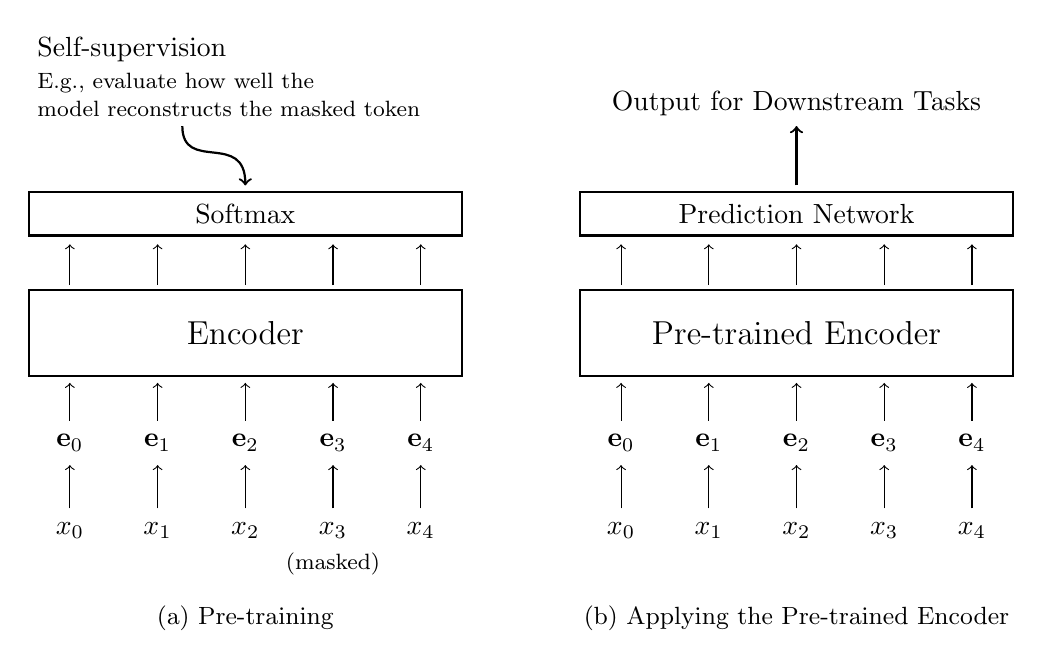
\begin{tikzpicture}
	
\def\nodewidth{0.55cm}
\def\nodeheight{0.55cm}

\tikzstyle{enode} = [minimum width=\nodewidth,minimum height=\nodeheight,inner sep=2pt];

%%% pre-training encoders
\begin{scope}

\node [enode,anchor=west] (w0) at (0,0) {$x_0$};
\node [enode,anchor=west] (w1) at ([xshift=\nodewidth]w0.east) {$x_1$};
\node [enode,anchor=west] (w2) at ([xshift=\nodewidth]w1.east) {$x_2$};
\node [enode,anchor=west] (w3) at ([xshift=\nodewidth]w2.east) {$x_3$};
\node [enode,anchor=west] (w4) at ([xshift=\nodewidth]w3.east) {$x_4$};
\node [enode,anchor=north] (w3mask) at ([yshift=0.4em]w3.south) {\footnotesize{(masked)}};

\node [enode,anchor=south] (e0) at ([yshift=\nodeheight]w0.north) {$\mathbf{e}_0$};
\node [enode,anchor=west] (e1) at ([xshift=\nodewidth]e0.east) {$\mathbf{e}_1$};
\node [enode,anchor=west] (e2) at ([xshift=\nodewidth]e1.east) {$\mathbf{e}_2$};
\node [enode,anchor=west] (e3) at ([xshift=\nodewidth]e2.east) {$\mathbf{e}_3$};
\node [enode,anchor=west] (e4) at ([xshift=\nodewidth]e3.east) {$\mathbf{e}_4$};

\draw [->] (w0.north) -- ([yshift=0]e0.south);
\draw [->] (w1.north) -- ([yshift=0]e1.south);
\draw [->] (w2.north) -- ([yshift=0]e2.south);
\draw [->] (w3.north) -- ([yshift=0]e3.south);
\draw [->] (w4.north) -- ([yshift=0]e4.south);

\node [anchor=south,minimum width=10*\nodewidth,minimum height=2*\nodeheight,draw,thick] (encoder) at ([yshift=\nodeheight]e2.north) {\large{Encoder}};

\draw [->] ([yshift=0pt]e0.north) -- ([yshift=\nodeheight-2pt]e0.north);
\draw [->] ([yshift=0pt]e1.north) -- ([yshift=\nodeheight-2pt]e1.north);
\draw [->] ([yshift=0pt]e2.north) -- ([yshift=\nodeheight-2pt]e2.north);
\draw [->] ([yshift=0pt]e3.north) -- ([yshift=\nodeheight-2pt]e3.north);
\draw [->] ([yshift=0pt]e4.north) -- ([yshift=\nodeheight-2pt]e4.north);

\draw [->] ([yshift=3*\nodeheight+2pt]e0.north) -- ([yshift=3*\nodeheight+1.2*\nodeheight-2pt]e0.north);
\draw [->] ([yshift=3*\nodeheight+2pt]e1.north) -- ([yshift=3*\nodeheight+1.2*\nodeheight-2pt]e1.north);
\draw [->] ([yshift=3*\nodeheight+2pt]e2.north) -- ([yshift=3*\nodeheight+1.2*\nodeheight-2pt]e2.north);
\draw [->] ([yshift=3*\nodeheight+2pt]e3.north) -- ([yshift=3*\nodeheight+1.2*\nodeheight-2pt]e3.north);
\draw [->] ([yshift=3*\nodeheight+2pt]e4.north) -- ([yshift=3*\nodeheight+1.2*\nodeheight-2pt]e4.north);

\node [anchor=south,minimum width=10*\nodewidth,minimum height=\nodeheight,draw,thick] (softmax) at ([yshift=1.2*\nodeheight]encoder.north) {Softmax};

\node [anchor=south west] (supervision1) at ([yshift=1.5*\nodeheight]softmax.north west) {\footnotesize{model reconstructs the masked token}};
\node [anchor=south west] (supervision2) at ([yshift=-0.4em]supervision1.north west) {\footnotesize{E.g., evaluate how well the}};
\node [anchor=south west] (supervision3) at ([yshift=-0.3em]supervision2.north west) {Self-supervision};

\draw [->,thick] ([yshift=1.5*\nodeheight,xshift=-0.8cm]softmax.north) .. controls +(south:0.6cm) and +(north:0.7cm) .. ([yshift=2pt]softmax.north);

\node [anchor=north] (caption) at ([yshift=-\nodeheight]w2.south) {\small{(a) Pre-training}};

\end{scope}

%%% applying pre-trained encoders
\begin{scope}[xshift=7cm]

\node [enode,anchor=west] (w0) at (0,0) {$x_0$};
\node [enode,anchor=west] (w1) at ([xshift=\nodewidth]w0.east) {$x_1$};
\node [enode,anchor=west] (w2) at ([xshift=\nodewidth]w1.east) {$x_2$};
\node [enode,anchor=west] (w3) at ([xshift=\nodewidth]w2.east) {$x_3$};
\node [enode,anchor=west] (w4) at ([xshift=\nodewidth]w3.east) {$x_4$};

\node [enode,anchor=south] (e0) at ([yshift=\nodeheight]w0.north) {$\mathbf{e}_0$};
\node [enode,anchor=west] (e1) at ([xshift=\nodewidth]e0.east) {$\mathbf{e}_1$};
\node [enode,anchor=west] (e2) at ([xshift=\nodewidth]e1.east) {$\mathbf{e}_2$};
\node [enode,anchor=west] (e3) at ([xshift=\nodewidth]e2.east) {$\mathbf{e}_3$};
\node [enode,anchor=west] (e4) at ([xshift=\nodewidth]e3.east) {$\mathbf{e}_4$};

\draw [->] (w0.north) -- ([yshift=0]e0.south);
\draw [->] (w1.north) -- ([yshift=0]e1.south);
\draw [->] (w2.north) -- ([yshift=0]e2.south);
\draw [->] (w3.north) -- ([yshift=0]e3.south);
\draw [->] (w4.north) -- ([yshift=0]e4.south);

\node [anchor=south,minimum width=10*\nodewidth,minimum height=2*\nodeheight,draw,thick] (encoder) at ([yshift=\nodeheight]e2.north) {\large{Pre-trained Encoder}};

\draw [->] ([yshift=0]e0.north) -- ([yshift=\nodeheight-2pt]e0.north);
\draw [->] ([yshift=0]e1.north) -- ([yshift=\nodeheight-2pt]e1.north);
\draw [->] ([yshift=0]e2.north) -- ([yshift=\nodeheight-2pt]e2.north);
\draw [->] ([yshift=0]e3.north) -- ([yshift=\nodeheight-2pt]e3.north);
\draw [->] ([yshift=0]e4.north) -- ([yshift=\nodeheight-2pt]e4.north);

\draw [->] ([yshift=3*\nodeheight+2pt]e0.north) -- ([yshift=3*\nodeheight+1.2*\nodeheight-2pt]e0.north);
\draw [->] ([yshift=3*\nodeheight+2pt]e1.north) -- ([yshift=3*\nodeheight+1.2*\nodeheight-2pt]e1.north);
\draw [->] ([yshift=3*\nodeheight+2pt]e2.north) -- ([yshift=3*\nodeheight+1.2*\nodeheight-2pt]e2.north);
\draw [->] ([yshift=3*\nodeheight+2pt]e3.north) -- ([yshift=3*\nodeheight+1.2*\nodeheight-2pt]e3.north);
\draw [->] ([yshift=3*\nodeheight+2pt]e4.north) -- ([yshift=3*\nodeheight+1.2*\nodeheight-2pt]e4.north);

\node [anchor=south,minimum width=10*\nodewidth,minimum height=\nodeheight,draw,thick] (softmax) at ([yshift=1.2*\nodeheight]encoder.north) {Prediction Network};

\node [anchor=south] (supervision1) at ([yshift=1.5*\nodeheight]softmax.north) {Output for Downstream Tasks};

\draw [->,thick] ([yshift=2pt]softmax.north) -- (supervision1.south);

\node [anchor=north] (caption) at ([yshift=-\nodeheight]w2.south) {\small{(b) Applying the Pre-trained Encoder}};

\end{scope}
	
\end{tikzpicture}

\caption{Pre-training a Transformer encoder (left) and then applying the pre-trained encoder (right). In the pre-training phase, the encoder, together with a Softmax layer, is trained via self-supervision. In the application phase, the Softmax layer is removed, and the pre-trained encoder is combined with a prediction network to address specific problems. In general, for better adaptation to these tasks, the system is fine-tuned using labeled data.}
\label{fig:pre-training-encoder-architecture}
\end{figure}

\noindent Here $\mathbf{p}_i^{\mathbf{W},\theta}$ is the output distribution $\Pr(\cdot|\mathbf{x})$ at position $i$. We use $\mathrm{Softmax}_{\mathbf{W}}(\cdot)$ to denote that the Softmax layer is parameterized by $\mathbf{W}$, that is, $\mathrm{Softmax}_{\mathbf{W}}(\mathbf{H}) = \mathrm{Softmax}(\mathbf{H} \cdot \mathbf{W})$. For notational simplicity, we will sometimes drop the superscripts $\mathbf{W}$ and $\theta$ affixed to each probability distribution.

The difference between this model and standard language models is that the output $\mathbf{p}_i$ has different meanings in encoder pre-training and language modeling. In language modeling, $\mathbf{p}_i$ is the probability distribution of predicting the next token. This follows an autoregressive decoding process: a language model only observes the words up to position $i$ and predicts the next. By contrast, in encoder pre-training, the entire sequence is observed at once, and thus it is trivial to predict a token when the model has already seen it.

\subsubsection{Masked Language Modeling}

\noindent One of the most popular methods of encoder pre-training is \mindex{masked language modeling}, which forms the basis of the well-known BERT model~\cite{devlin-etal:2019bert}. The idea of masked language modeling is to create prediction challenges by masking out some of the tokens in the input sequence and training a model to predict the masked tokens. In this sense, the conventional language modeling problem, which is sometimes called \mindex{causal language modeling}, is a special case of masked language modeling: at each position, we mask the tokens in the right context, and predict the token at this position using its left context. However, in causal language modeling, only the left context is used for token prediction, and the model does not have access to tokens in the right context. By contrast, in masked language modeling, all the unmasked tokens are used for word prediction, leading to a bidirectional model that makes predictions based on both left and right contexts.

More formally, for an input sequence $\mathbf{x}=x_0\cdots x_m$, suppose that we mask the tokens at positions $\mathcal{A}(\mathbf{x}) = \{i_1,\cdots,i_{u}\}$. Hence we obtain a masked token sequence $\bar{\mathbf{x}}$ where the token at each position in $\mathcal{A}(\mathbf{x})$ is replaced with a special symbol $[\mathrm{MASK}]$. For example, for the following sequence

\vspace{0.5em}
\begin{center}
The early bird catches the worm
\end{center}
\vspace{0.5em}

\noindent we may have a masked token sequence like this

\vspace{0.5em}
\begin{center}
The $[\mathrm{MASK}]$ bird catches the $[\mathrm{MASK}]$
\end{center}
\vspace{0.5em}

\noindent where we mask the tokens \textit{early} and \textit{worm} (i.e., $i_1 = 2$ and $i_2 = 6$).

Now we have two sequences $\mathbf{x}$ and $\bar{\mathbf{x}}$. The model is then optimized so that we can correctly predict $\mathbf{x}$ based on $\bar{\mathbf{x}}$. This can be thought of as an autoencoding-like process, and the training objective is to maximize the reconstruction probability $\Pr(\mathbf{x}|\bar{\mathbf{x}})$. Note that there is a simple position-wise alignment between $\mathbf{x}$ and $\bar{\mathbf{x}}$. Because an unmasked token in $\bar{\mathbf{x}}$ is the same as the token in $\mathbf{x}$ at the same position, there is no need to consider the prediction for this unmasked token. This leads to a simplified training objective which only maximizes the probabilities for masked tokens. We can express this objective in a maximum likelihood estimation fashion
\begin{eqnarray}
(\widehat{\mathbf{W}},\hat{\theta}) & = & \argmax_{\mathbf{W},\theta} \sum_{\mathbf{x} \in \mathcal{D}} \sum_{i \in \mathcal{A}(\mathbf{x})} \log \mathrm{Pr}_{i}^{\mathbf{W},\theta}(x_{i}|\bar{\mathbf{x}}),
\end{eqnarray}

\noindent or alternatively express it using the cross-entropy loss
\begin{eqnarray}
(\widehat{\mathbf{W}},\hat{\theta}) & = & \argmin_{\mathbf{W},\theta} \sum_{\mathbf{x} \in \mathcal{D}} \sum_{i \in \mathcal{A}(\mathbf{x})} \mathrm{CrossEntropy}(\mathbf{p}_{i}^{\mathbf{W},\theta},\mathbf{p}_{i}^{\mathrm{gold}}),
\end{eqnarray}

\noindent where $\mathrm{Pr}_k^{\mathbf{W},\theta}(x_k|\bar{\mathbf{x}})$ is the probability of the true token $x_k$ at position $k$ given the corrupted input $\bar{\mathbf{x}}$, and $\mathbf{p}_{k}^{\mathbf{W},\theta}$ is the probability distribution at position $k$ given the corrupted input $\bar{\mathbf{x}}$. To illustrate, consider the above example where two tokens of the sequence ``\textit{the early bird catches the worm}'' are masked. For this example, the objective is to maximize the sum of log-probabilities
\begin{eqnarray}
\mathrm{Loss} & = & \log \Pr(x_2 = \textit{early}|\bar{\mathbf{x}}=\textit{$[\mathrm{CLS}]$ The $\underbrace{[\mathrm{MASK}]}_{\bar{x}_2}$ bird catches the $\underbrace{[\mathrm{MASK}]}_{\bar{x}_6}$}) + \nonumber \\
  &   & \log \Pr(x_6 = \textit{worm}|\bar{\mathbf{x}}=\textit{$[\mathrm{CLS}]$ The $\underbrace{[\mathrm{MASK}]}_{\bar{x}_2}$ bird catches the $\underbrace{[\mathrm{MASK}]}_{\bar{x}_6}$}).
\end{eqnarray}

Once we obtain the optimized parameters $\widehat{\mathbf{W}}$ and $\hat{\theta}$, we can drop $\widehat{\mathbf{W}}$. Then, we can further fine-tune the pre-trained encoder $\mathrm{Encode}_{\hat{\theta}}(\cdot)$ or directly apply it to downstream tasks.

\subsubsection{Permuted Language Modeling}

\noindent While masked language modeling is simple and widely applied, it introduces new issues. One drawback is the use of a special token, $[\mathrm{MASK}]$, which is employed only during training but not at test time. This leads to a discrepancy between training and inference. Moreover, the auto-encoding process overlooks the dependencies between masked tokens. For example, in the previously discussed example, the prediction of $x_2$ (i.e., the first masked token) is made independently of $x_6$ (i.e., the second masked token), even though $x_6$ and $x_2$ are interdependent in the context of the sentence.

These issues can be addressed using the \mindex{permuted language modeling} approach to pre-training~\cite{yang-etal:2019xlnet}. Similar to causal language modeling, permuted language modeling involves making sequential predictions of tokens. However, unlike causal modeling where predictions follow the natural sequence of the text (like left-to-right or right-to-left), permuted language modeling allows for predictions in any order. The approach is straightforward: we determine an order for token predictions and then train the model in a standard language modeling manner, as described in Section~\ref{sec:decoder-only-pre-training}. Note that in this approach, the actual order of tokens in the text remains unchanged, and only the order in which we predict these tokens differs from standard language modeling. For example, consider a sequence of 5 tokens $x_0 x_1 x_2 x_3 x_4$. Let $\mathbf{e}_i$ represent the embedding of $x_i$ (i.e., combination of the token embedding and positional embedding). In standard language modeling, we would generate this sequence in the order of $x_0 \to x_1 \to x_2 \to x_3 \to x_4$. The probability of the sequence can be modeled via a generation process.
\begin{eqnarray}
\Pr(\mathbf{x}) & = & \Pr(x_0) \cdot \Pr(x_1|x_0) \cdot \Pr(x_2|x_0,x_1) \cdot \Pr(x_3|x_0,x_1,x_2) \cdot \nonumber \\
                &   & \Pr(x_4|x_0,x_1,x_2,x_3).
\end{eqnarray}

\noindent In practice, the model conditions on token embeddings rather than the tokens themselves. Therefore, we can rewrite the above expression as
\begin{eqnarray}
\Pr(\mathbf{x}) & = & \Pr(x_0) \cdot \Pr(x_1|\mathbf{e}_0) \cdot \Pr(x_2|\mathbf{e}_0,\mathbf{e}_1) \cdot \Pr(x_3|\mathbf{e}_0,\mathbf{e}_1, \mathbf{e}_2) \cdot \nonumber \\
                &   & \Pr(x_4|\mathbf{e}_0, \mathbf{e}_1, \mathbf{e}_2, \mathbf{e}_3).
\end{eqnarray}


Now, let us consider a different order for token prediction: $x_0 \to x_4 \to x_2 \to x_1 \to x_3$. The sequence generation process can then be expressed as follows:
\begin{eqnarray}
\Pr(\mathbf{x}) & = & \Pr(x_0) \cdot \Pr(x_4|\mathbf{e}_0) \cdot \Pr(x_2|\mathbf{e}_0, \mathbf{e}_4) \cdot \Pr(x_1|\mathbf{e}_0, \mathbf{e}_4, \mathbf{e}_2) \cdot \nonumber \\
                &   & \Pr(x_3|\mathbf{e}_0, \mathbf{e}_4, \mathbf{e}_2, \mathbf{e}_1) \label{eq:permuted-factorization-lm-example}.
\end{eqnarray}

This new prediction order allows some tokens to be generated based on a broader context, rather than being limited to just the preceding tokens as in standard language models. For example, in generating $x_3$, the model considers both its left context (i.e., $\{\mathbf{e}_0, \mathbf{e}_1, \mathbf{e}_2\}$) and right context (i.e., $\{\mathbf{e}_4\}$). The embeddings $\mathbf{e}_0, \mathbf{e}_1, \mathbf{e}_2, \mathbf{e}_4$ incorporate the positional information of $x_0, x_1, x_2, x_4$, preserving the original order of the tokens. As a result, this approach is somewhat akin to masked language modeling: we mask out $x_3$ and use its surrounding tokens $x_0, x_1, x_2, x_4$ to predict this token.

The implementation of permuted language models is relatively easy for Transformers. Because self-attention itself is permutation-invariant, and positional information is encoded separately using positional embeddings, we do not need to explicitly reorder the input sequence to have a factorization like Eq. (\ref{eq:permuted-factorization-lm-example}). Instead, permutation can be done by setting appropriate masks for self-attention. For example, consider the step of computing $\Pr(x_1 | \mathbf{e}_0, \mathbf{e}_4, \mathbf{e}_2)$. We can keep $x_0, x_1, x_2, x_3, x_4$ in their original positions and simply prevent $x_1$ from attending to $x_3$ during the self-attention computation, as illustrated below

\begin{center}
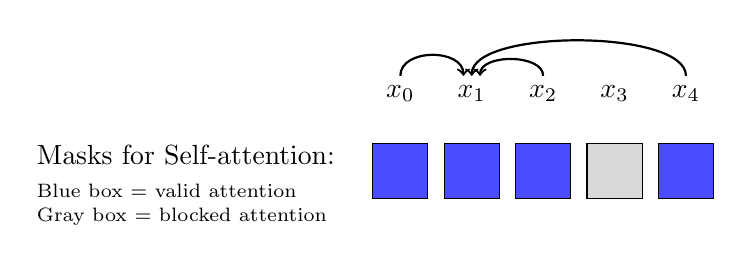
\begin{tikzpicture}
\def\nodesize{0.7cm}
\node [] (x0) at (0,0) {$x_0$};
\node [anchor=west] (x1) at ([xshift=0.3cm]x0.east) {$x_1$};
\node [anchor=west] (x2) at ([xshift=0.3cm]x1.east) {$x_2$};
\node [anchor=west] (x3) at ([xshift=0.3cm]x2.east) {$x_3$};
\node [anchor=west] (x4) at ([xshift=0.3cm]x3.east) {$x_4$};
\draw [->,thick] (x0.north) .. controls +(north:1em) and +(north:1em) .. ([xshift=-0.3em]x1.north);
\draw [->,thick] (x2.north) .. controls +(north:0.8em) and +(north:0.8em) .. ([xshift=0.3em]x1.north);
\draw [->,thick] (x4.north) .. controls +(north:1.7em) and +(north:1.7em) .. ([xshift=0.0em]x1.north);

\node [anchor=north,minimum width=\nodesize,minimum height=\nodesize,draw,fill=blue!70] (box0) at ([yshift=-0.4cm]x0.south) {};
\node [anchor=north,minimum width=\nodesize,minimum height=\nodesize,draw,fill=blue!70] (box1) at ([yshift=-0.4cm]x1.south) {};
\node [anchor=north,minimum width=\nodesize,minimum height=\nodesize,draw,fill=blue!70] (box2) at ([yshift=-0.4cm]x2.south) {};
\node [anchor=north,minimum width=\nodesize,minimum height=\nodesize,draw,fill=gray!30] (box3) at ([yshift=-0.4cm]x3.south) {};
\node [anchor=north,minimum width=\nodesize,minimum height=\nodesize,draw,fill=blue!70] (box4) at ([yshift=-0.4cm]x4.south) {};

\node [anchor=east] (label) at ([xshift=-1em,yshift=0.6em]box0.west) {Masks for Self-attention:};
\node [anchor=north west] (label1) at (label.south west) {\scriptsize{Blue box = valid attention}};
\node [anchor=north west] (label2) at ([yshift=0.3em]label1.south west) {\scriptsize{Gray box = blocked attention}};
\end{tikzpicture}
\end{center}

\noindent For a clearer illustration, we compare the self-attention masking results of causal language modeling, masked language modeling and permuted language modeling in Figure~\ref{fig:comparison-of-masking-for-pre-training-lms}.

\begin{figure}[!t]
\centering
% !Mode:: "TeX:UTF-8"
% !TEX encoding = UTF-8 Unicode

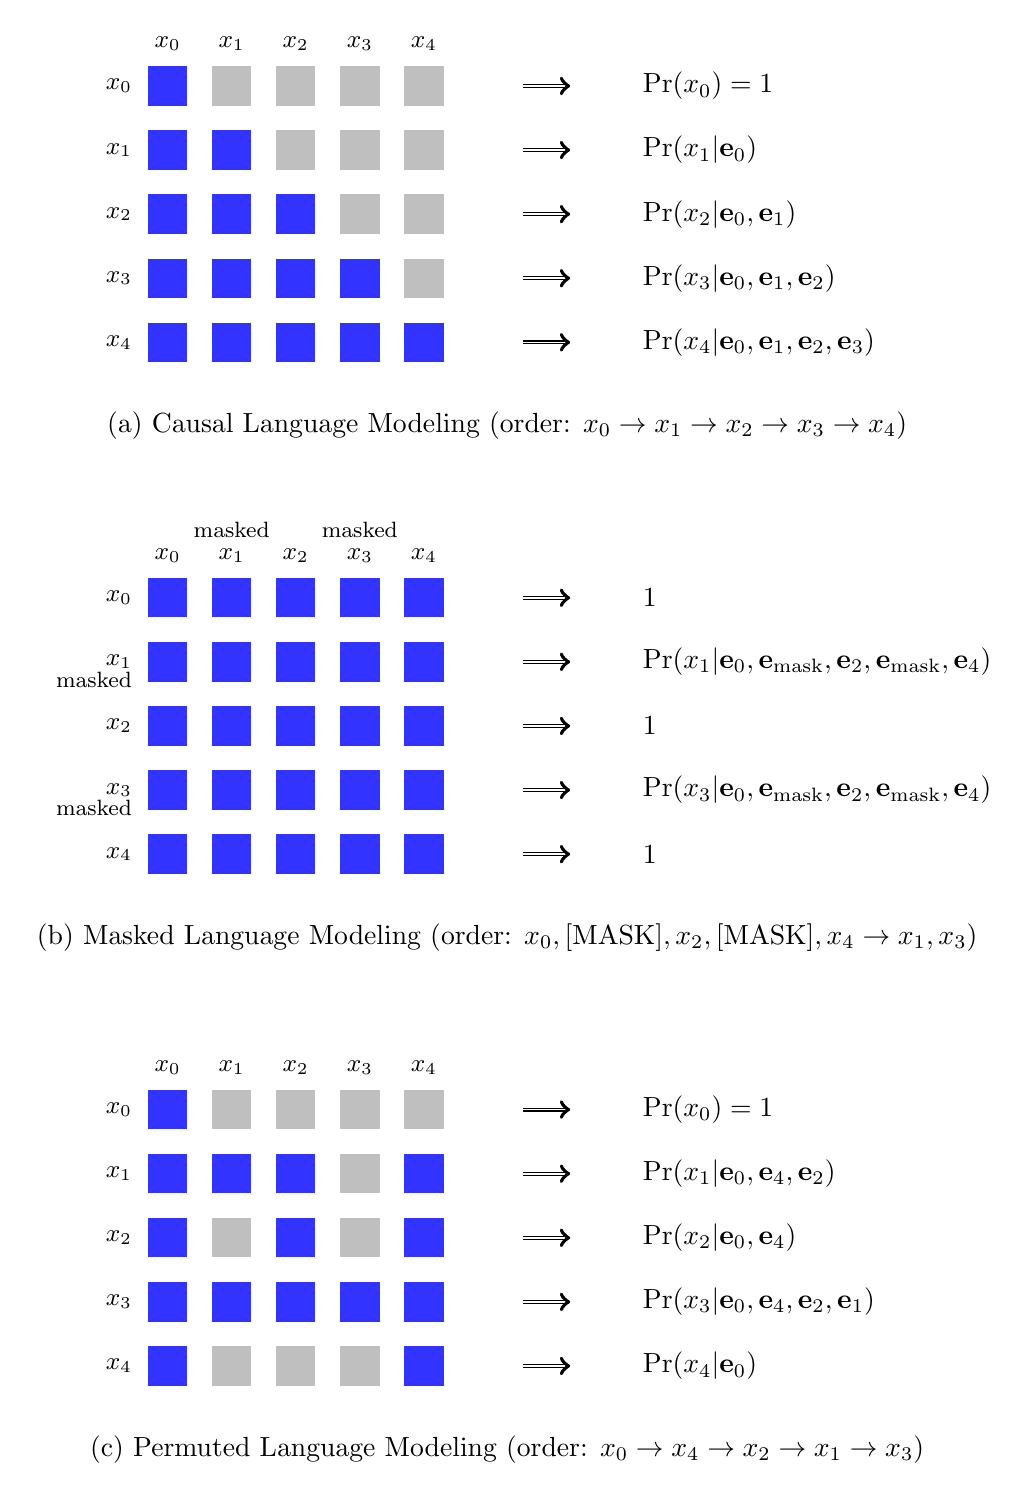
\begin{tikzpicture}
	
\def\nodewidth{0.5cm}
\def\nodeheight{0.5cm}
\def\nodestep{0.6*\nodewidth}

\tikzstyle{enode} = [minimum width=\nodewidth,minimum height=\nodeheight,inner sep=2pt,fill=gray!50];

%%% causal language modeling
\begin{scope}

\node [enode,anchor=west,fill=blue!80] (node00) at (0,0) {};
\node [enode,anchor=west] (node01) at ([xshift=\nodestep]node00.east) {};
\node [enode,anchor=west] (node02) at ([xshift=\nodestep]node01.east) {};
\node [enode,anchor=west] (node03) at ([xshift=\nodestep]node02.east) {};
\node [enode,anchor=west] (node04) at ([xshift=\nodestep]node03.east) {};
\node [enode,anchor=north,fill=blue!80] (node10) at ([yshift=-\nodestep]node00.south) {};
\node [enode,anchor=west,fill=blue!80] (node11) at ([xshift=\nodestep]node10.east) {};
\node [enode,anchor=west] (node12) at ([xshift=\nodestep]node11.east) {};
\node [enode,anchor=west] (node13) at ([xshift=\nodestep]node12.east) {};
\node [enode,anchor=west] (node14) at ([xshift=\nodestep]node13.east) {};
\node [enode,anchor=north,fill=blue!80] (node20) at ([yshift=-\nodestep]node10.south) {};
\node [enode,anchor=west,fill=blue!80] (node21) at ([xshift=\nodestep]node20.east) {};
\node [enode,anchor=west,fill=blue!80] (node22) at ([xshift=\nodestep]node21.east) {};
\node [enode,anchor=west] (node23) at ([xshift=\nodestep]node22.east) {};
\node [enode,anchor=west] (node24) at ([xshift=\nodestep]node23.east) {};
\node [enode,anchor=north,fill=blue!80] (node30) at ([yshift=-\nodestep]node20.south) {};
\node [enode,anchor=west,fill=blue!80] (node31) at ([xshift=\nodestep]node30.east) {};
\node [enode,anchor=west,fill=blue!80] (node32) at ([xshift=\nodestep]node31.east) {};
\node [enode,anchor=west,fill=blue!80] (node33) at ([xshift=\nodestep]node32.east) {};
\node [enode,anchor=west] (node34) at ([xshift=\nodestep]node33.east) {};
\node [enode,anchor=north,fill=blue!80] (node40) at ([yshift=-\nodestep]node30.south) {};
\node [enode,anchor=west,fill=blue!80] (node41) at ([xshift=\nodestep]node40.east) {};
\node [enode,anchor=west,fill=blue!80] (node42) at ([xshift=\nodestep]node41.east) {};
\node [enode,anchor=west,fill=blue!80] (node43) at ([xshift=\nodestep]node42.east) {};
\node [enode,anchor=west,fill=blue!80] (node44) at ([xshift=\nodestep]node43.east) {};

\foreach \i in {0,...,4}{
    \node [anchor=south] (hx\i) at ([yshift=0.2em]node0\i.north) {\small{$x_{\i}$}};
    \node [anchor=east] (vx\i) at ([xshift=-0.2em]node\i0.west) {\small{$x_{\i}$}};
    \draw [->,double] ([xshift=1.0cm]node\i4.east) -- ([xshift=1.6cm]node\i4.east);
}

\node [anchor=west] (pr0) at ([xshift=2.4cm]node04.east) {$\Pr(x_0)=1$};
\node [anchor=west] (pr1) at ([xshift=2.4cm]node14.east) {$\Pr(x_1|\mathbf{e}_0)$};
\node [anchor=west] (pr2) at ([xshift=2.4cm]node24.east) {$\Pr(x_2|\mathbf{e}_0,\mathbf{e}_1)$};
\node [anchor=west] (pr3) at ([xshift=2.4cm]node34.east) {$\Pr(x_3|\mathbf{e}_0,\mathbf{e}_1,\mathbf{e}_2)$};
\node [anchor=west] (pr4) at ([xshift=2.4cm]node44.east) {$\Pr(x_4|\mathbf{e}_0,\mathbf{e}_1,\mathbf{e}_2,\mathbf{e}_3)$};

\node [anchor=north] (caption) at ([yshift=-0.5cm,xshift=0.8cm]node44.south east) {(a) Causal Language Modeling (order: $x_0 \to x_1 \to x_2 \to x_3 \to x_4$)};

\end{scope}

%%% masked language modeling
\begin{scope}[yshift=-6.5cm]

\node [enode,anchor=west,fill=blue!80] (node00) at (0,0) {};
\node [enode,anchor=west,fill=blue!80] (node01) at ([xshift=\nodestep]node00.east) {};
\node [enode,anchor=west,fill=blue!80] (node02) at ([xshift=\nodestep]node01.east) {};
\node [enode,anchor=west,fill=blue!80] (node03) at ([xshift=\nodestep]node02.east) {};
\node [enode,anchor=west,fill=blue!80] (node04) at ([xshift=\nodestep]node03.east) {};
\node [enode,anchor=north,fill=blue!80] (node10) at ([yshift=-\nodestep]node00.south) {};
\node [enode,anchor=west,fill=blue!80] (node11) at ([xshift=\nodestep]node10.east) {};
\node [enode,anchor=west,fill=blue!80] (node12) at ([xshift=\nodestep]node11.east) {};
\node [enode,anchor=west,fill=blue!80] (node13) at ([xshift=\nodestep]node12.east) {};
\node [enode,anchor=west,fill=blue!80] (node14) at ([xshift=\nodestep]node13.east) {};
\node [enode,anchor=north,fill=blue!80] (node20) at ([yshift=-\nodestep]node10.south) {};
\node [enode,anchor=west,fill=blue!80] (node21) at ([xshift=\nodestep]node20.east) {};
\node [enode,anchor=west,fill=blue!80] (node22) at ([xshift=\nodestep]node21.east) {};
\node [enode,anchor=west,fill=blue!80] (node23) at ([xshift=\nodestep]node22.east) {};
\node [enode,anchor=west,fill=blue!80] (node24) at ([xshift=\nodestep]node23.east) {};
\node [enode,anchor=north,fill=blue!80] (node30) at ([yshift=-\nodestep]node20.south) {};
\node [enode,anchor=west,fill=blue!80] (node31) at ([xshift=\nodestep]node30.east) {};
\node [enode,anchor=west,fill=blue!80] (node32) at ([xshift=\nodestep]node31.east) {};
\node [enode,anchor=west,fill=blue!80] (node33) at ([xshift=\nodestep]node32.east) {};
\node [enode,anchor=west,fill=blue!80] (node34) at ([xshift=\nodestep]node33.east) {};
\node [enode,anchor=north,fill=blue!80] (node40) at ([yshift=-\nodestep]node30.south) {};
\node [enode,anchor=west,fill=blue!80] (node41) at ([xshift=\nodestep]node40.east) {};
\node [enode,anchor=west,fill=blue!80] (node42) at ([xshift=\nodestep]node41.east) {};
\node [enode,anchor=west,fill=blue!80] (node43) at ([xshift=\nodestep]node42.east) {};
\node [enode,anchor=west,fill=blue!80] (node44) at ([xshift=\nodestep]node43.east) {};

\foreach \i in {0,...,4}{
    \node [anchor=south] (hx\i) at ([yshift=0.2em]node0\i.north) {\small{$x_{\i}$}};
    \node [anchor=east] (vx\i) at ([xshift=-0.2em]node\i0.west) {\small{$x_{\i}$}};
    \draw [->,double] ([xshift=1.0cm]node\i4.east) -- ([xshift=1.6cm]node\i4.east);
}

\node [anchor=south] (hmasked3) at ([yshift=-0.1cm]hx3.north) {\footnotesize{masked}};
\node [anchor=south] (hmasked1) at ([yshift=-0.1cm]hx1.north) {\footnotesize{masked}};
\node [anchor=north east] (vmasked3) at ([yshift=0.2cm]vx3.south east) {\footnotesize{masked}};
\node [anchor=north east] (vmasked1) at ([yshift=0.2cm]vx1.south east) {\footnotesize{masked}};

\node [anchor=west] (pr0) at ([xshift=2.4cm]node04.east) {$1$};
\node [anchor=west] (pr1) at ([xshift=2.4cm]node14.east) {$\Pr(x_1|\mathbf{e}_0,\mathbf{e}_{\mathrm{mask}},\mathbf{e}_2,\mathbf{e}_{\mathrm{mask}},\mathbf{e}_4)$};
\node [anchor=west] (pr2) at ([xshift=2.4cm]node24.east) {$1$};
\node [anchor=west] (pr3) at ([xshift=2.4cm]node34.east) {$\Pr(x_3|\mathbf{e}_0,\mathbf{e}_{\mathrm{mask}},\mathbf{e}_2,\mathbf{e}_{\mathrm{mask}},\mathbf{e}_4)$};
\node [anchor=west] (pr4) at ([xshift=2.4cm]node44.east) {$1$};

\node [anchor=north] (caption) at ([yshift=-0.5cm,xshift=0.8cm]node44.south east) {(b) Masked Language Modeling (order: $x_0, \mathrm{[MASK]}, x_2, \mathrm{[MASK]}, x_4 \to x_1, x_3$)};

\end{scope}

%%% permuted language modeling
\begin{scope}[yshift=-13cm]

\node [enode,anchor=west,fill=blue!80] (node00) at (0,0) {};
\node [enode,anchor=west] (node01) at ([xshift=\nodestep]node00.east) {};
\node [enode,anchor=west] (node02) at ([xshift=\nodestep]node01.east) {};
\node [enode,anchor=west] (node03) at ([xshift=\nodestep]node02.east) {};
\node [enode,anchor=west] (node04) at ([xshift=\nodestep]node03.east) {};
\node [enode,anchor=north,fill=blue!80] (node10) at ([yshift=-\nodestep]node00.south) {};
\node [enode,anchor=west,fill=blue!80] (node11) at ([xshift=\nodestep]node10.east) {};
\node [enode,anchor=west,fill=blue!80] (node12) at ([xshift=\nodestep]node11.east) {};
\node [enode,anchor=west] (node13) at ([xshift=\nodestep]node12.east) {};
\node [enode,anchor=west,fill=blue!80] (node14) at ([xshift=\nodestep]node13.east) {};
\node [enode,anchor=north,fill=blue!80] (node20) at ([yshift=-\nodestep]node10.south) {};
\node [enode,anchor=west] (node21) at ([xshift=\nodestep]node20.east) {};
\node [enode,anchor=west,fill=blue!80] (node22) at ([xshift=\nodestep]node21.east) {};
\node [enode,anchor=west] (node23) at ([xshift=\nodestep]node22.east) {};
\node [enode,anchor=west,fill=blue!80] (node24) at ([xshift=\nodestep]node23.east) {};
\node [enode,anchor=north,fill=blue!80] (node30) at ([yshift=-\nodestep]node20.south) {};
\node [enode,anchor=west,fill=blue!80] (node31) at ([xshift=\nodestep]node30.east) {};
\node [enode,anchor=west,fill=blue!80] (node32) at ([xshift=\nodestep]node31.east) {};
\node [enode,anchor=west,fill=blue!80] (node33) at ([xshift=\nodestep]node32.east) {};
\node [enode,anchor=west,fill=blue!80] (node34) at ([xshift=\nodestep]node33.east) {};
\node [enode,anchor=north,fill=blue!80] (node40) at ([yshift=-\nodestep]node30.south) {};
\node [enode,anchor=west] (node41) at ([xshift=\nodestep]node40.east) {};
\node [enode,anchor=west] (node42) at ([xshift=\nodestep]node41.east) {};
\node [enode,anchor=west] (node43) at ([xshift=\nodestep]node42.east) {};
\node [enode,anchor=west,fill=blue!80] (node44) at ([xshift=\nodestep]node43.east) {};

\foreach \i in {0,...,4}{
    \node [anchor=south] (hx\i) at ([yshift=0.2em]node0\i.north) {\small{$x_{\i}$}};
    \node [anchor=east] (vx\i) at ([xshift=-0.2em]node\i0.west) {\small{$x_{\i}$}};
    \draw [->,double] ([xshift=1.0cm]node\i4.east) -- ([xshift=1.6cm]node\i4.east);
}

\node [anchor=west] (pr0) at ([xshift=2.4cm]node04.east) {$\Pr(x_0)=1$};
\node [anchor=west] (pr1) at ([xshift=2.4cm]node14.east) {$\Pr(x_1|\mathbf{e}_0,\mathbf{e}_4,\mathbf{e}_2)$};
\node [anchor=west] (pr2) at ([xshift=2.4cm]node24.east) {$\Pr(x_2|\mathbf{e}_0,\mathbf{e}_4)$};
\node [anchor=west] (pr3) at ([xshift=2.4cm]node34.east) {$\Pr(x_3|\mathbf{e}_0,\mathbf{e}_4,\mathbf{e}_2,\mathbf{e}_1)$};
\node [anchor=west] (pr4) at ([xshift=2.4cm]node44.east) {$\Pr(x_4|\mathbf{e}_0)$};

\node [anchor=north] (caption) at ([yshift=-0.5cm,xshift=0.8cm]node44.south east) {(c) Permuted Language Modeling (order: $x_0 \to x_4 \to x_2 \to x_1 \to x_3$)};

\end{scope}
	
\end{tikzpicture}

\caption{Comparison of self-attention masking results of causal language modeling, masked language modeling and permuted language modeling. The gray cell denotes that the token at position $j$ does not attend to the token at position $i$. The blue cell $(i,j)$ denotes that the token at position $j$ attends to the token at position $i$. $\mathbf{e}_{\mathrm{mask}}$ represents the embedding of the symbol $[\mathrm{MASK}]$, which is a combination of the token embedding and the positional embedding.}
\label{fig:comparison-of-masking-for-pre-training-lms}
\end{figure}

\subsubsection{Pre-training Encoders as Classifiers}
\label{sec:pre-training-as-classification}

\noindent Another common approach to training an encoder is to use classification tasks. In self-supervised learning, this is typically done by creating new classification challenges from the unlabeled text. There are many different ways to design the classification tasks. Here we present two popular tasks.

A simple method, called \mindex{next sentence prediction} (\mindex{NSP}), is presented in BERT's original paper~\cite{devlin-etal:2019bert}. NSP is based on the assumption that a good text encoder should capture the relationship between two sentences. To model this relationship, NSP uses the encoder output of two consecutive sentences $\mathrm{Sent}_{A}$ and $\mathrm{Sent}_{B}$ to determine whether $\mathrm{Sent}_{B}$ is the next sentence following $\mathrm{Sent}_{A}$. For example, suppose $\mathrm{Sent}_{A} = \textit{'It is raining .'}$ and $\mathrm{Sent}_{B} = \textit{'I need an umbrella .'}$. The input sequence of the encoder could be

\vspace{0.5em}
\begin{center}
$[\mathrm{CLS}]$ It is raining . $[\mathrm{SEP}]$ I need an umbrella . $[\mathrm{SEP}]$
\end{center}
\vspace{0.5em}

\noindent where $[\mathrm{CLS}]$ is the start symbol (i.e., $x_0$) which is commonly used in encoder pre-training, and $[\mathrm{SEP}]$ is a separator that separates the two sentences. The processing of this sequence follows a standard procedure of Transformer encoding: we first represent each token $x_i$ as its corresponding embedding $\mathbf{e}_i$, and then feed the embedding sequence $\{\mathbf{e}_{0},\cdots,\mathbf{e}_m\}$ into the encoder to obtain the output sequence $\{\mathbf{h}_{0},\cdots,\mathbf{h}_m\}$. Since $\mathbf{h}_{0}$ is generally considered as the representation of the entire sequence, we add a Softmax layer on top of it to construct a binary classification system. This process is illustrated as follows:

\vspace{0.5em}
\begin{center}
\begingroup
\renewcommand{\arraystretch}{1.2}
\setlength{\tabcolsep}{3pt}
\begin{tabular}{r c c c c c c c c c c c c}
token: & {\color{red} $[\mathrm{CLS}]$} & It & is & raining & . & $[\mathrm{SEP}]$ & I & need & an & umbrella & . & $[\mathrm{SEP}]$ \\
embedding: & {\color{red} $\mathbf{e}_0$} & $\mathbf{e}_1$ & $\mathbf{e}_2$ & $\mathbf{e}_3$ & $\mathbf{e}_4$ & $\mathbf{e}_5$ & $\mathbf{e}_6$ & $\mathbf{e}_7$ & $\mathbf{e}_8$ & $\mathbf{e}_9$ & $\mathbf{e}_{10}$ & $\mathbf{e}_{11}$ \\
 & {\color{red} $\downarrow$} & $\downarrow$ & $\downarrow$ & $\downarrow$ & $\downarrow$ & $\downarrow$ & $\downarrow$ & $\downarrow$ & $\downarrow$ & $\downarrow$ & $\downarrow$ & $\downarrow$ \\ \cline{2-13}
& \multicolumn{12}{|c|}{Encoder} \\ \cline{2-13}
 & {\color{red} $\downarrow$} & $\downarrow$ & $\downarrow$ & $\downarrow$ & $\downarrow$ & $\downarrow$ & $\downarrow$ & $\downarrow$ & $\downarrow$ & $\downarrow$ & $\downarrow$ & $\downarrow$ \\
 encoding: & {\color{red} $\mathbf{h}_0$} & $\mathbf{h}_1$ & $\mathbf{h}_2$ & $\mathbf{h}_3$ & $\mathbf{h}_4$ & $\mathbf{h}_5$ & $\mathbf{h}_6$ & $\mathbf{h}_7$ & $\mathbf{h}_8$ & $\mathbf{h}_9$ & $\mathbf{h}_{10}$ & $\mathbf{h}_{11}$ \\
 & $\downarrow$ \\
 & \multicolumn{3}{l}{Softmax} \\
 & $\downarrow$ \\
 & \multicolumn{3}{l}{Is Next or Not?}
\end{tabular}
\endgroup
\end{center}
\vspace{0.5em}

To generate training samples, we extract sentence pairs from a text corpus. A positive sample is created by selecting two actual consecutive sentences, while a negative sample is formed by pairing a sentence with a randomly chosen sentence from the corpus. As a result, training this model is the same as training a classifier. Typically, NSP is used as an additional training loss function for pre-training based on masked language modeling.

A second approach to training Transformer encoders as classifiers applies classification-based supervision signals at the token level. For example, \citet{clark-etal:2019electra} propose, in their ELECTRA model, training a Transformer encoder to identify whether each input token is identical to the original token or has been altered in some manner. The first step of this method is to generate a new sequence from a given sequence of tokens, where some of the tokens are altered. To do this, a small masked language model (call it the generator) is applied: we randomly mask some of the tokens, and train this model to predict the masked tokens. For each training sample, this masked language model outputs a token at each masked position, which may differ from the original token. At the same time, we train another Transformer encoder (call it the discriminator) to determine whether each predicted token is the same as the original token or altered. More specifically, we use the generator to generate a sequence where some of the tokens are replaced. Below is an illustration.

\vspace{0.5em}
\begin{center}
\begingroup
\renewcommand{\arraystretch}{1.2}
\begin{tabular}{r c c c c c c c c c}
original: & $[\mathrm{CLS}]$ & The & boy & spent & hours & working & on & toys & . \\
& $\downarrow$ & $\downarrow$ & $\downarrow$ & $\downarrow$ & $\downarrow$ & $\downarrow$ & $\downarrow$ & $\downarrow$ & $\downarrow$ \\
masked: & $[\mathrm{CLS}]$ & The & boy & spent & {\color{red} $[\mathrm{MASK}]$} & working & on & {\color{red} $[\mathrm{MASK}]$} & . \\
& $\downarrow$ & $\downarrow$ & $\downarrow$ & $\downarrow$ & {\color{red} $\downarrow$} & $\downarrow$ & $\downarrow$ & {\color{red} $\downarrow$} & $\downarrow$ \\ \cline{2-10}
& \multicolumn{9}{|c|}{Generator (small masked language model)} \\ \cline{2-10}
& $\downarrow$ & $\downarrow$ & $\downarrow$ & $\downarrow$ & {\color{red} $\downarrow$} & $\downarrow$ & $\downarrow$ & {\color{red} $\downarrow$} & $\downarrow$ \\
replaced: & $[\mathrm{CLS}]$ & The & boy & spent & {\color{red} decades} & working & on & {\color{red} toys} & .
\end{tabular}
\endgroup
\end{center}
\vspace{0.5em}

Then, we use the discriminator to label each of these tokens as $\mathrm{original}$ or $\mathrm{replaced}$, as follows

\vspace{0.5em}
\begin{center}
\begingroup
\renewcommand{\arraystretch}{1.2}
\setlength{\tabcolsep}{3pt}
\begin{tabular}{r c c c c c c c c c}
replaced: & $[\mathrm{CLS}]$ & The & boy & spent & {\color{red} decades} & working & on & {\color{red} toys} & . \\
& $\downarrow$ & $\downarrow$ & $\downarrow$ & $\downarrow$ & {\color{red} $\downarrow$} & $\downarrow$ & $\downarrow$ & {\color{red} $\downarrow$} & $\downarrow$ \\ \cline{2-10}
& \multicolumn{9}{|c|}{Discriminator (the model we want)} \\ \cline{2-10}
& $\downarrow$ & $\downarrow$ & $\downarrow$ & $\downarrow$ & {\color{red} $\downarrow$} & $\downarrow$ & $\downarrow$ & {\color{red} $\downarrow$} & $\downarrow$ \\
label: & \footnotesize{$\mathrm{original}$} & \footnotesize{$\mathrm{original}$} & \footnotesize{$\mathrm{original}$} & \footnotesize{$\mathrm{original}$} & {\color{red} \footnotesize{$\mathrm{replaced}$}} & \footnotesize{$\mathrm{original}$} & \footnotesize{$\mathrm{original}$} & {\color{red} \footnotesize{$\mathrm{original}$}} & \footnotesize{$\mathrm{original}$}
\end{tabular}
\endgroup
\end{center}
\vspace{0.5em}

For training, the generator is optimized as a masked language model with maximum likelihood estimation, and the discriminator is optimized as a classifier using a classification-based loss. In ELECTRA, the maximum likelihood-based loss and the classification-based loss are combined for jointly training both the generator and discriminator. An alternative approach is to use generative adversarial networks (GANs), that is, the generator is trained to fool the discriminator, and the discriminator is trained to distinguish the output of the generator from the true distribution. However, GAN-style training complicates the training task and is more difficult to scale up. Nevertheless, once training is complete, the generator is discarded, and the encoding part of the discriminator is applied as the pre-trained model for downstream tasks.

\subsection{Encoder-Decoder Pre-training}

\noindent In NLP, encoder-decoder architectures are often used to model sequence-to-sequence problems, such as machine translation and question answering. In addition to these typical sequence-to-sequence problems in NLP, encoder-decoder models can be extended to deal with many other problems. A simple idea is to treat text as both the input and output of a problem, and so we can directly apply encoder-decoder models. For example, given an input text, we can instruct a model to generate text describing its sentiment (e.g., \textit{positive}, \textit{negative}, or \textit{neutral}).

Such an idea allows us to develop a single text-to-text system to address any NLP problem. We can formulate different problems into the same text-to-text format. We first train an encoder-decoder model to gain general-purpose knowledge of language via self-supervision. This model is then fine-tuned for specific downstream tasks using targeted text-to-text data.

\subsubsection{Masked Encoder-Decoder Pre-training}

\noindent In \citet{raffel-etal:2020exploring}'s \mindex{T5} model, many different tasks are framed as the same text-to-text task. Each sample in T5 follows the format
\begin{eqnarray}
\textrm{Source Text} & \to & \textrm{Target Text} \nonumber
\end{eqnarray}

\noindent Here $\to$ separates the source text, which consists of a task description or instruction and the input given to the system, from the target text, which is the response to the input task. As an example, consider a task of translating from Chinese to English. A training sample can be expressed as:
\begin{eqnarray}
[\mathrm{CLS}]\ \textrm{Translate from Chinese to English: \begin{CJK*}{UTF8}{gbsn}你好！\end{CJK*}} & \to & \langle s \rangle\ \textrm{Hello!} \nonumber
\end{eqnarray}

\noindent where $[\mathrm{CLS}]$ and $\langle s \rangle$ are the start symbols on the source and target sides, respectively\footnote{We could use the same start symbol for different sequences. Here we use different symbols to distinguish between the sequences on the encoder and decoder-sides.}.

Likewise, we can express other tasks in the same way. For example
\begin{eqnarray}
&     & \mathrm{[CLS]}\ \textrm{\colorbox{gray!30}{Answer:} when was Albert Einstein born?} \nonumber \\
& \to & \langle s \rangle\ \textrm{He was born on March 14, 1879.} \nonumber \\
&     & \nonumber \\
&     & \mathrm{[CLS]}\ \textrm{\colorbox{gray!30}{Simplify:} the professor, who has published numerous papers in his field,} \nonumber \\
&     & \textrm{will be giving a lecture on the topic next week.} \nonumber \\
& \to & \langle s \rangle\ \textrm{The experienced professor will give a lecture next week.} \nonumber \\
&     & \nonumber \\
&     & \mathrm{[CLS]}\ \textrm{\colorbox{gray!30}{Text:} John bought a new car. Hypothesis: John has a car.} \nonumber \\
& \to & \langle s \rangle\ \textrm{Entailment} \nonumber \\
&     & \nonumber \\
&     & \mathrm{[CLS]}\ \textrm{\colorbox{gray!30}{Score the translation from English to Chinese.} English: when in Rome, do as} \nonumber \\
&     & \textrm{ the Romans do. Chinese: \begin{CJK*}{UTF8}{gbsn}人\ 在\ 罗马\ 就\ 像\ 罗马\ 人\ 一样\ 做事\ 。\end{CJK*}} \nonumber \\
& \to & \langle s \rangle\ 0.81 \nonumber
\end{eqnarray}

\noindent where instructions are highlighted in gray. Interestingly, in the last example, we frame a continuous scoring problem as a text generation task. Our goal is to generate the text string representing the number $0.81$, rather than outputting a continuous numerical value.

The approach described above provides a new framework of universal language understanding and generation. Both the task instructions and the problem inputs are provided to the system in text form. The system then follows the instructions to complete the task. This method puts different problems together, with the benefit of training a single model that can perform many tasks simultaneously.

In general, fine-tuning is necessary for adapting the pre-trained model to a specific downstream task. In this process, one can use different ways to instruct the model for the task, such as using a short name of the task as the prefix to the actual input sequence or providing a detailed description of the task. Because task instructions are provided as text and processed as part of the input, general instruction-following capabilities can be acquired during the pre-training phase. This greatly facilitates zero-shot learning. For instance, pre-trained models can often generalize to solve new problems where task-specific instructions have never been encountered during training.

There have been several powerful methods of self-supervised learning for either Transformer encoders or decoders. Applying these methods to pre-train encoder-decoder models is relatively straightforward. One common choice is to train encoder-decoder models as language models. For example, the encoder receives a sequence prefix, while the decoder generates the remaining sequence. However, this differs from standard causal language modeling, where the entire sequence is autoregressively generated from the first token. In our case, the encoder processes the prefix at once, and then the decoder predicts subsequent tokens in the manner of causal language modeling. Put more precisely, this is a \mindex{prefix language modeling} problem: a language model predicts the subsequent sequence given a prefix, which serves as the context for prediction.

Consider the following example
\begin{eqnarray}
\underbrace{\mathrm{[CLS]}\ \textrm{The puppies are frolicking}}_{\textrm{Prefix}} & \to & \underbrace{\langle s \rangle\ \textrm{outside the house .}}_{\textrm{Subsequent Sequence}} \nonumber
\end{eqnarray}

\noindent We can directly train an encoder-decoder model using examples like this. Then, the encoder learns to understand the prefix, and the decoder learns to continue writing based on this understanding. For large-scale pre-training, it is easy to create a large number of training examples from unlabeled text.

It is worth noting that for pre-trained encoder-decoder models to be effective in multilingual and cross-lingual tasks (e.g., machine translation), they should be trained on multilingual data. This typically requires that the vocabulary includes tokens from multiple languages. By doing so, the models can learn shared representations across different languages, thereby enabling capabilities in both language understanding and generation in a multilingual and cross-lingual context.

A second approach to pre-training encoder-decoder models is masked language modeling. In this approach, as discussed in Section~\ref{sec:encoder-only-pre-training}, tokens in a sequence are randomly replaced with a mask symbol, and the model is then trained to predict these masked tokens based on the corrupted sequence.

As an illustration, consider the task of masking and reconstructing the sentence

\vspace{0.5em}
\begin{center}
The puppies are frolicking outside the house .
\end{center}
\vspace{0.5em}

\noindent By masking two tokens (say, \textit{frolicking} and \textit{the}), we have the BERT-style input and output of the model, as follows
\begin{eqnarray}
&     & \mathrm{[CLS]}\ \textrm{The puppies are $\mathrm{[MASK]}$ outside $\mathrm{[MASK]}$ house .} \nonumber \\
& \to & \langle s \rangle\ \textrm{\underline{\hspace{1em}}\ \ \underline{\hspace{1em}}\ \ \underline{\hspace{1em}}\ \ frolicking\ \ \underline{\hspace{1em}}\ \ the \underline{\hspace{1em}}\ \ \underline{\hspace{1em}}} \nonumber
\end{eqnarray}

\noindent Here \underline{\hspace{1em}} denotes the masked position at which we do not make token predictions. By varying the percentage of the tokens in the text, this approach can be generalized towards either BERT-style training or language modeling-style training~\cite{song-etal:2019mass}. For example, if we mask out all the tokens, then the model is trained to generate the entire sequence
\begin{eqnarray}
&     & \mathrm{[CLS]}\ \textrm{$\mathrm{[MASK]}$ $\mathrm{[MASK]}$ $\mathrm{[MASK]}$ $\mathrm{[MASK]}$ $\mathrm{[MASK]}$ $\mathrm{[MASK]}$ $\mathrm{[MASK]}$ $\mathrm{[MASK]}$} \nonumber \\
& \to & \langle s \rangle\ \textrm{The puppies are frolicking outside the house .} \nonumber
\end{eqnarray}

\noindent In this case, we train the decoder as a language model.

Note that, in the context of the encoder-decoder architecture, we can use the encoder to read the masked sequence, and use the decoder to predict the original sequence. With this objective, we essentially have a denoising autoencoder: the encoder transforms a corrupted input into some hidden representation, and the decoder reconstructs the uncorrupted input from this hidden representation. Here is an example of input and output for denoising training.

\begin{eqnarray}
&     & \mathrm{[CLS]}\ \textrm{The puppies are $\mathrm{[MASK]}$ outside $\mathrm{[MASK]}$ house .} \nonumber \\
& \to & \langle s \rangle\ \textrm{The puppies are frolicking outside the house .} \nonumber
\end{eqnarray}

\noindent By learning to map from this corrupted sequence to its uncorrupted counterpart, the model gains the ability to understand on the encoder side and to generate on the decoder side. See Figure~\ref{fig:encoder-decoder-masked-lm} for an illustration of how an encoder-decoder model is trained with BERT-style and denoising autoencoding objectives.

\begin{figure}[!t]
\centering
% !Mode:: "TeX:UTF-8"
% !TEX encoding = UTF-8 Unicode

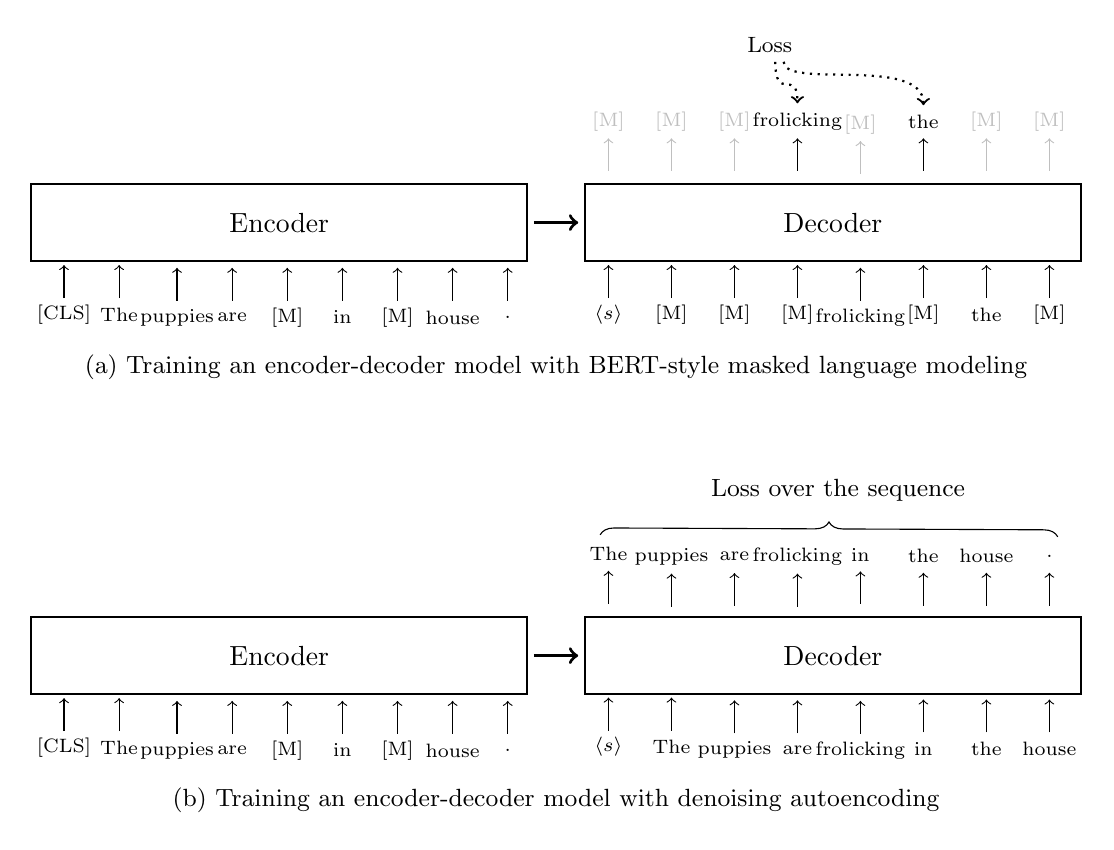
\begin{tikzpicture}
	
\def\nodestep{0.7cm}
\def\bignodestep{0.8cm}

\tikzstyle{enode} = [minimum width=9*\nodestep,minimum height=1.4*\nodestep,inner sep=2pt,draw,thick];

%%% training an encoder-decoder model with masked language modeling
\begin{scope}

\node [anchor=center] (x0) at (0,0) {\scriptsize{$\mathrm{[CLS]}$}};
\node [anchor=center] (x1) at ([xshift=\nodestep]x0.center) {\scriptsize{The}};
\node [anchor=center] (x2) at ([xshift=\nodestep+1pt,yshift=-1pt]x1.center) {\scriptsize{puppies}};
\node [anchor=center] (x3) at ([xshift=\nodestep]x2.center) {\scriptsize{are}};
\node [anchor=center] (x4) at ([xshift=\nodestep]x3.center) {\scriptsize{$\mathrm{[M]}$}};
\node [anchor=center] (x5) at ([xshift=\nodestep]x4.center) {\scriptsize{in}};
\node [anchor=center] (x6) at ([xshift=\nodestep]x5.center) {\scriptsize{$\mathrm{[M]}$}};
\node [anchor=center] (x7) at ([xshift=\nodestep]x6.center) {\scriptsize{house}};
\node [anchor=center] (x8) at ([xshift=\nodestep]x7.center) {\scriptsize{.}};

\draw [->] ([yshift=0.6em]x0.center) -- ([yshift=\nodestep-2pt]x0.center);
\draw [->] ([yshift=0.6em]x1.center) -- ([yshift=\nodestep-2pt]x1.center);
\draw [->] ([yshift=0.6em]x2.center) -- ([yshift=\nodestep-2pt]x2.center);
\draw [->] ([yshift=0.6em]x3.center) -- ([yshift=\nodestep-2pt]x3.center);
\draw [->] ([yshift=0.6em]x4.center) -- ([yshift=\nodestep-2pt]x4.center);
\draw [->] ([yshift=0.6em]x5.center) -- ([yshift=\nodestep-2pt]x5.center);
\draw [->] ([yshift=0.6em]x6.center) -- ([yshift=\nodestep-2pt]x6.center);
\draw [->] ([yshift=0.6em]x7.center) -- ([yshift=\nodestep-2pt]x7.center);
\draw [->] ([yshift=0.6em]x8.center) -- ([yshift=\nodestep-2pt]x8.center);

\node [enode,anchor=south] (encoder) at ([xshift=1.3*\nodestep,yshift=\nodestep]x3.west) {Encoder};
\node [enode,anchor=west] (decoder) at ([xshift=2em]encoder.east) {Decoder};

\draw [->,very thick] ([xshift=2pt]encoder.east) -- ([xshift=-2pt]decoder.west);

\node [anchor=center] (y4) at ([yshift=-\nodestep,xshift=0.5*\nodestep]decoder.south) {\scriptsize{frolicking}};
\node [anchor=center] (y3) at ([xshift=-\bignodestep,yshift=0.1em]y4.center) {\scriptsize{$\mathrm{[M]}$}};
\node [anchor=center] (y2) at ([xshift=-\bignodestep]y3.center) {\scriptsize{$\mathrm{[M]}$}};
\node [anchor=center] (y1) at ([xshift=-\bignodestep]y2.center) {\scriptsize{$\mathrm{[M]}$}};
\node [anchor=center] (y0) at ([xshift=-\bignodestep]y1.center) {\scriptsize{$\langle s \rangle$}};
\node [anchor=center] (y5) at ([xshift=\bignodestep,yshift=0.1em]y4.center) {\scriptsize{$\mathrm{[M]}$}};
\node [anchor=center] (y6) at ([xshift=\bignodestep]y5.center) {\scriptsize{the}};
\node [anchor=center] (y7) at ([xshift=\bignodestep]y6.center) {\scriptsize{$\mathrm{[M]}$}};

\draw [->] ([yshift=0.6em]y0.center) -- ([yshift=\nodestep-2pt]y0.center);
\draw [->] ([yshift=0.6em]y1.center) -- ([yshift=\nodestep-2pt]y1.center);
\draw [->] ([yshift=0.6em]y2.center) -- ([yshift=\nodestep-2pt]y2.center);
\draw [->] ([yshift=0.6em]y3.center) -- ([yshift=\nodestep-2pt]y3.center);
\draw [->] ([yshift=0.6em]y4.center) -- ([yshift=\nodestep-2pt]y4.center);
\draw [->] ([yshift=0.6em]y5.center) -- ([yshift=\nodestep-2pt]y5.center);
\draw [->] ([yshift=0.6em]y6.center) -- ([yshift=\nodestep-2pt]y6.center);
\draw [->] ([yshift=0.6em]y7.center) -- ([yshift=\nodestep-2pt]y7.center);

\node [anchor=center] (o0) at ([yshift=3.5*\nodestep]y0.center) {\scriptsize{{\color{gray!50} $\mathrm{[M]}$}}};
\node [anchor=center] (o1) at ([yshift=3.5*\nodestep]y1.center) {\scriptsize{{\color{gray!50} $\mathrm{[M]}$}}};
\node [anchor=center] (o2) at ([yshift=3.5*\nodestep]y2.center) {\scriptsize{{\color{gray!50} $\mathrm{[M]}$}}};
\node [anchor=center] (o3) at ([yshift=3.5*\nodestep]y3.center) {\scriptsize{frolicking}};
\node [anchor=center] (o4) at ([yshift=3.5*\nodestep]y4.center) {\scriptsize{{\color{gray!50} $\mathrm{[M]}$}}};
\node [anchor=center] (o5) at ([yshift=3.5*\nodestep]y5.center) {\scriptsize{the}};
\node [anchor=center] (o6) at ([yshift=3.5*\nodestep]y6.center) {\scriptsize{{\color{gray!50} $\mathrm{[M]}$}}};
\node [anchor=center] (o7) at ([yshift=3.5*\nodestep]y7.center) {\scriptsize{{\color{gray!50} $\mathrm{[M]}$}}};

\draw [<-,gray!50] ([yshift=-0.6em]o0.center) -- ([yshift=-\nodestep+2pt]o0.center);
\draw [<-,gray!50] ([yshift=-0.6em]o1.center) -- ([yshift=-\nodestep+2pt]o1.center);
\draw [<-,gray!50] ([yshift=-0.6em]o2.center) -- ([yshift=-\nodestep+2pt]o2.center);
\draw [<-] ([yshift=-0.6em]o3.center) -- ([yshift=-\nodestep+2pt]o3.center);
\draw [<-,gray!50] ([yshift=-0.6em]o4.center) -- ([yshift=-\nodestep+2pt]o4.center);
\draw [<-] ([yshift=-0.6em]o5.center) -- ([yshift=-\nodestep+2pt]o5.center);
\draw [<-,gray!50] ([yshift=-0.6em]o6.center) -- ([yshift=-\nodestep+2pt]o6.center);
\draw [<-,gray!50] ([yshift=-0.6em]o7.center) -- ([yshift=-\nodestep+2pt]o7.center);

\node [anchor=south] (loss) at ([yshift=1.5em,xshift=-1em]o3.north) {\footnotesize{Loss}};

\draw [->,thick,dotted] ([yshift=-0.0em,xshift=0.2em]loss.south) .. controls +(south:1.5em) and +(north:1.3em) .. ([yshift=0.0em]o3.north);
\draw [->,thick,dotted] ([yshift=-0.0em,xshift=0.5em]loss.south) .. controls +(south:1em) and +(north:1.8em) .. ([yshift=0.0em]o5.north);

\node [anchor=north] (caption) at ([xshift=1em,yshift=-3em]encoder.south east) {\small{(a) Training an encoder-decoder model with BERT-style masked language modeling}};

\end{scope}

%%% training an encoder-decoder model with denosing autoencoding methods
\begin{scope}[yshift=-5.5cm]

\node [anchor=center] (x0) at (0,0) {\scriptsize{$\mathrm{[CLS]}$}};
\node [anchor=center] (x1) at ([xshift=\nodestep]x0.center) {\scriptsize{The}};
\node [anchor=center] (x2) at ([xshift=\nodestep+1pt,yshift=-1pt]x1.center) {\scriptsize{puppies}};
\node [anchor=center] (x3) at ([xshift=\nodestep]x2.center) {\scriptsize{are}};
\node [anchor=center] (x4) at ([xshift=\nodestep]x3.center) {\scriptsize{$\mathrm{[M]}$}};
\node [anchor=center] (x5) at ([xshift=\nodestep]x4.center) {\scriptsize{in}};
\node [anchor=center] (x6) at ([xshift=\nodestep]x5.center) {\scriptsize{$\mathrm{[M]}$}};
\node [anchor=center] (x7) at ([xshift=\nodestep]x6.center) {\scriptsize{house}};
\node [anchor=center] (x8) at ([xshift=\nodestep]x7.center) {\scriptsize{.}};

\draw [->] ([yshift=0.6em]x0.center) -- ([yshift=\nodestep-2pt]x0.center);
\draw [->] ([yshift=0.6em]x1.center) -- ([yshift=\nodestep-2pt]x1.center);
\draw [->] ([yshift=0.6em]x2.center) -- ([yshift=\nodestep-2pt]x2.center);
\draw [->] ([yshift=0.6em]x3.center) -- ([yshift=\nodestep-2pt]x3.center);
\draw [->] ([yshift=0.6em]x4.center) -- ([yshift=\nodestep-2pt]x4.center);
\draw [->] ([yshift=0.6em]x5.center) -- ([yshift=\nodestep-2pt]x5.center);
\draw [->] ([yshift=0.6em]x6.center) -- ([yshift=\nodestep-2pt]x6.center);
\draw [->] ([yshift=0.6em]x7.center) -- ([yshift=\nodestep-2pt]x7.center);
\draw [->] ([yshift=0.6em]x8.center) -- ([yshift=\nodestep-2pt]x8.center);

\node [enode,anchor=south] (encoder) at ([xshift=1.3*\nodestep,yshift=\nodestep]x3.west) {Encoder};
\node [enode,anchor=west] (decoder) at ([xshift=2em]encoder.east) {Decoder};

\draw [->,very thick] ([xshift=2pt]encoder.east) -- ([xshift=-2pt]decoder.west);

\node [anchor=center] (y4) at ([yshift=-\nodestep,xshift=0.5*\nodestep]decoder.south) {\scriptsize{frolicking}};
\node [anchor=center] (y3) at ([xshift=-\bignodestep,yshift=0.02em]y4.center) {\scriptsize{are}};
\node [anchor=center] (y2) at ([xshift=-\bignodestep]y3.center) {\scriptsize{puppies}};
\node [anchor=center] (y1) at ([xshift=-\bignodestep,yshift=0.1em]y2.center) {\scriptsize{The}};
\node [anchor=center] (y0) at ([xshift=-\bignodestep]y1.center) {\scriptsize{$\langle s \rangle$}};
\node [anchor=center] (y5) at ([xshift=\bignodestep,yshift=0.05em]y4.center) {\scriptsize{in}};
\node [anchor=center] (y6) at ([xshift=\bignodestep]y5.center) {\scriptsize{the}};
\node [anchor=center] (y7) at ([xshift=\bignodestep]y6.center) {\scriptsize{house}};

\draw [->] ([yshift=0.6em]y0.center) -- ([yshift=\nodestep-2pt]y0.center);
\draw [->] ([yshift=0.6em]y1.center) -- ([yshift=\nodestep-2pt]y1.center);
\draw [->] ([yshift=0.6em]y2.center) -- ([yshift=\nodestep-2pt]y2.center);
\draw [->] ([yshift=0.6em]y3.center) -- ([yshift=\nodestep-2pt]y3.center);
\draw [->] ([yshift=0.6em]y4.center) -- ([yshift=\nodestep-2pt]y4.center);
\draw [->] ([yshift=0.6em]y5.center) -- ([yshift=\nodestep-2pt]y5.center);
\draw [->] ([yshift=0.6em]y6.center) -- ([yshift=\nodestep-2pt]y6.center);
\draw [->] ([yshift=0.6em]y7.center) -- ([yshift=\nodestep-2pt]y7.center);

\node [anchor=center] (o0) at ([yshift=3.5*\nodestep]y0.center) {\scriptsize{The}};
\node [anchor=center] (o1) at ([yshift=3.5*\nodestep-1pt]y1.center) {\scriptsize{puppies}};
\node [anchor=center] (o2) at ([yshift=3.5*\nodestep+0.02em]y2.center) {\scriptsize{are}};
\node [anchor=center] (o3) at ([yshift=3.5*\nodestep]y3.center) {\scriptsize{frolicking}};
\node [anchor=center] (o4) at ([yshift=3.5*\nodestep+0.1em]y4.center) {\scriptsize{in}};
\node [anchor=center] (o5) at ([yshift=3.5*\nodestep]y5.center) {\scriptsize{the}};
\node [anchor=center] (o6) at ([yshift=3.5*\nodestep]y6.center) {\scriptsize{house}};
\node [anchor=center] (o7) at ([yshift=3.5*\nodestep]y7.center) {\scriptsize{.}};

\draw [<-] ([yshift=-0.6em]o0.center) -- ([yshift=-\nodestep+2pt]o0.center);
\draw [<-] ([yshift=-0.6em]o1.center) -- ([yshift=-\nodestep+2pt]o1.center);
\draw [<-] ([yshift=-0.6em]o2.center) -- ([yshift=-\nodestep+2pt]o2.center);
\draw [<-] ([yshift=-0.6em]o3.center) -- ([yshift=-\nodestep+2pt]o3.center);
\draw [<-] ([yshift=-0.6em]o4.center) -- ([yshift=-\nodestep+2pt]o4.center);
\draw [<-] ([yshift=-0.6em]o5.center) -- ([yshift=-\nodestep+2pt]o5.center);
\draw [<-] ([yshift=-0.6em]o6.center) -- ([yshift=-\nodestep+2pt]o6.center);
\draw [<-] ([yshift=-0.6em]o7.center) -- ([yshift=-\nodestep+2pt]o7.center);


\node [anchor=north] (caption) at ([xshift=1em,yshift=-3em]encoder.south east) {\small{(b) Training an encoder-decoder model with denoising autoencoding}};

\node [anchor=south] (loss) at ([yshift=1em,xshift=-0.5em]o3.north east) {\small{Loss over the sequence}};

\draw [decoration={brace,amplitude=5pt},decorate] ([yshift=0.7em,xshift=-0.3em]o0.center) -- ([yshift=0.7em,xshift=0.3em]o7.center);

\end{scope}
	
\end{tikzpicture}

\caption{Training an encoder-decoder model using BERT-style and denoising autoencoding methods. In both methods, the input to the encoder is a corrupted token sequence where some tokens are masked and replaced with $\mathrm{[MASK]}$ (or $\mathrm{[M]}$ for short). The decoder predicts these masked tokens, but in different ways. In BERT-style training, the decoder only needs to compute the loss for the masked tokens, while the remaining tokens in the sequence can be simply treated as $\mathrm{[MASK]}$ tokens. In denoising autoencoding, the decoder predicts the sequence of all tokens in an autoregressive manner.  As a result, the loss is obtained by accumulating the losses of all these tokens, as in standard language modeling.}
\label{fig:encoder-decoder-masked-lm}
\end{figure}

As we randomly select tokens for masking, we can mask consecutive tokens~\cite{joshi-etal:2020spanbert}. Here is an example.
\begin{eqnarray}
&     & \mathrm{[CLS]}\ \textrm{The puppies are $\mathrm{[MASK]}$ outside $\mathrm{[MASK]}$ $\mathrm{[MASK]}$ .} \nonumber \\
& \to & \langle s \rangle\ \textrm{The puppies are frolicking outside the house .} \nonumber
\end{eqnarray}

Another way to consider consecutive masked tokens is to represent them as spans. Here we follow \citet{raffel-etal:2020exploring}'s work, and use $\mathrm{[X]}$, $\mathrm{[Y]}$ and $\mathrm{[Z]}$ to denote sentinel tokens that cover one or more consecutive masked tokens. Using this notation, we can re-express the above training example as:
\begin{eqnarray}
&     & \mathrm{[CLS]}\ \textrm{The puppies are $\mathrm{[X]}$ outside $\mathrm{[Y]}$ .} \nonumber \\
& \to & \langle s \rangle\ \textrm{$\mathrm{[X]}$ frolicking $\mathrm{[Y]}$ the house $\mathrm{[Z]}$} \nonumber
\end{eqnarray}

The idea is that we represent the corrupted sequence as a sequence containing placeholder slots. The training task is to fill these slots with the correct tokens using the surrounding context. An advantage of this approach is that the sequences used in training would be shorter, making the training more efficient. Note that masked language modeling provides a very general framework for training encoder-decoder models. Various settings can be adjusted to have different training versions, such as altering the percentage of tokens masked and the maximum length of the masked spans.

\subsubsection{Denoising Training}

\noindent If we view encoder-decoder pre-training as a denoising autoencoding problem, there are many ways to corrupt the input. For instance, beyond random token masking, we can also modify tokens or rearrange their order.

Suppose we have an encoder-decoder model that can map an input sequence $\mathbf{x}$ to an output sequence $\mathbf{y}$
\begin{eqnarray}
\mathbf{y} & = & \mathrm{Decode}_{\omega}(\mathrm{Encode}_{\theta}(\mathbf{x})) \nonumber \\
           & = & \mathrm{Model}_{\theta,\omega}(\mathbf{x}),
\end{eqnarray}

\noindent where $\theta$ and $\omega$ are the parameters of the encoder and the decoder, respectively. In denoising autoencoding, we add some noise to $\mathbf{x}$ to obtain a noisy, corrupted input $\mathbf{x}_{\mathrm{noise}}$. By feeding $\mathbf{x}_{\mathrm{noise}}$ into the encoder, the decoder is trained to recontruct the original input. The training objective can be defined as:
\begin{eqnarray}
(\hat{\theta},\hat{\omega}) & = & \argmin_{\theta,\omega} \mathrm{Loss}(\mathrm{Model}_{\theta,\omega}(\mathbf{x}_{\mathrm{noise}}),\mathbf{x}),
\end{eqnarray}

\noindent Here the loss function $\mathrm{Loss}(\mathrm{Model}_{\theta,\omega}(\mathbf{x}_{\mathrm{noise}}),\mathbf{x})$ evaluates how well the model $\mathrm{Model}_{\theta,\omega}(\mathbf{x}_{\mathrm{noise}})$ reconstructs the original input $\mathbf{x}$. We can choose the cross-entropy loss as usual.

Given the model architecture and training framework, the remaining issue is how to corrupt the input. \citet{lewis-etal:2020bart}, in their \mindex{BART} model, propose several ways to corrupt the input sequence.

\begin{itemize}
\item \vspace{0.5em} \mindex{Token Masking}. This is the same masking method that we used in masked language modeling. Tokens are randomly selected and replaced with $\mathrm{[MASK]}$.
\item \vspace{0.3em} \mindex{Token Deletion}. This method is similar to token masking. However, rather than replacing the selected tokens with a special symbol $\mathrm{[MASK]}$, these tokens are removed from the sequence. See the following example for a comparison of the token masking and token deletion methods.

    \begin{center}
    \begingroup
    %\setlength{\tabsep}{4pt}
    \renewcommand{\arraystretch}{1.2}
    \begin{tabular}{r l}
    Original ($\mathbf{x}$): & The puppies are \underline{frolicking} outside \underline{the} house . \\
    Token Masking ($\mathbf{x}_{\mathrm{noise}}$): & The puppies are $\mathrm{[MASK]}$ outside $\mathrm{[MASK]}$ house . \\
    Token Deletion ($\mathbf{x}_{\mathrm{noise}}$): & The puppies are {\color{gray} \sout{frolicking}} outside {\color{gray} \sout{the}} house .
    \end{tabular}
    \endgroup
    \end{center}

    \noindent where the underlined tokens in the original sequence are masked or deleted.

\item \vspace{0.3em} \mindex{Span Masking}. Non-overlapping spans are randomly sampled over the sequence. Each span is masked by $\mathrm{[MASK]}$. We also allow spans of length 0, and, in such cases, $\mathrm{[MASK]}$ is simply inserted at a position in the sequence. For example, we can use span masking to corrupt the above sequence as

    \begin{center}
    \begingroup
    \renewcommand{\arraystretch}{1.2}
    \begin{tabular}{r l}
    Original ($\mathbf{x}$): & The \underline{0} puppies are \underline{frolicking outside the} house . \\
    Span Masking ($\mathbf{x}_{\mathrm{noise}}$): & The $\mathrm{[MASK]}$ puppies are $\mathrm{[MASK]}$ house .
    \end{tabular}
    \endgroup
    \end{center}

    \noindent Here the span \textit{frolicking outside the} is replaced with a single $\mathrm{[MASK]}$. $\underline{0}$ indicates a length-0 span, and so we insert an $\mathrm{[MASK]}$ between \textit{The} and \textit{puppies}. Span masking introduces new prediction challenges in which the model needs to know how many tokens are generated from a span. This problem is very similar to fertility modeling in machine translation~\cite{brown-etal:1993mathematics}.
\end{itemize}
\vspace{0.5em}

If we consider a sequence consisting of multiple sentences, additional methods of corruption can be applied. In the BART model, there are two such methods.

\begin{itemize}
\item \vspace{0.5em} \mindex{Sentence Reordering}. This method randomly permutes the sentences so that the model can learn to reorder sentences in a document. Consider, for example, two consecutive sentences

    \begin{center}
    Hard work leads to success . Success brings happiness .
    \end{center}

    We can reorder the two sentences to have a corrupted input sequence

    \begin{center}
    Success brings happiness . Hard work leads to success .
    \end{center}

\item \vspace{0.3em} \mindex{Document Rotation}. The goal of this task is to identify the start token of the sequence. First, a token is randomly selected from the sequence. Then, the sequence is rotated so that the selected token is the first token. For example, suppose we select the token \textit{leads} from the above sequence. The rotated sequence is

    \begin{center}
    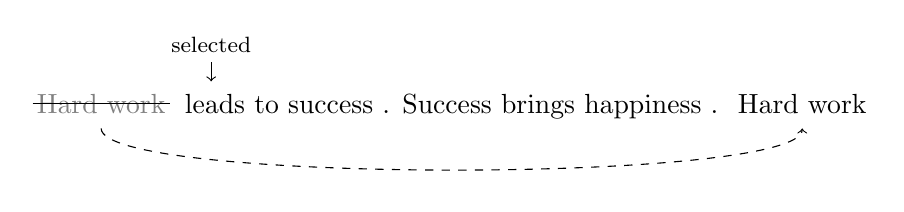
\begin{tikzpicture}
    \node [anchor=west] (seg1) at (0,0) {leads to success . Success brings happiness .};
    \node [anchor=east] (seg0) at ([yshift=0.1em]seg1.west) {{\color{gray} Hard work}};
    \node [anchor=west] (seg2) at ([yshift=0.1em]seg1.east) {Hard work};
    \draw [-] ([xshift=0.2em]seg0.west) -- ([xshift=-0.2em]seg0.east);
    \draw [->,dashed] ([yshift=-0.2em]seg0.south) .. controls +(south:2em) and +(south:2em) .. ([yshift=-0.2em]seg2.south);
    \node [anchor=south] (selected) at ([xshift=1.3em,yshift=0.8em]seg1.north west) {\footnotesize{selected}};
    \draw [->] (selected.south) -- ([yshift=-0.7em]selected.south);
    \end{tikzpicture}
    \end{center}

    \noindent where the subsequence \textit{Hard work} before \textit{leads} is appended to the end of the sequence.

\end{itemize}
\vspace{0.5em}

For pre-training, we can apply multiple corruption methods to learn robust models, for example, we randomly choose one of them for each training sample. In practice, the outcome of encoder-decoder pre-training depends heavily on the input corruption methods used, and so we typically need to choose appropriate training objectives through careful experimentation.

\subsection{Comparison of Pre-training Tasks}

\noindent So far, we have discussed a variety of pre-training tasks. Because the same training objective can often be applied to different architectures (e.g., using masked language modeling for both encoder-only and encoder-decoder pre-training), categorizing these tasks solely based on model architecture is insufficient. Instead, we summarize them based on their training objectives.

\begin{itemize}
\item \vspace{0.5em} \textbf{Language Modeling}. Typically, this approach refers to an autoregressive process of sequence generation. At each step, the model predicts the next token based exclusively on its preceding context.
\item \vspace{0.3em} \textbf{Masked Language Modeling}. Masked language modeling follows a general mask-predict framework. It randomly masks tokens in a sequence and predicts these tokens using the entire masked sequence.
\item \vspace{0.3em} \textbf{Permuted Language Modeling}. Permuted language modeling shares similarities with masked language modeling but removes the fixed left-to-right restriction by permuting the factorization order. It keeps the input sequence fixed but reorders the factorization (prediction) order. Each prediction is based on some context tokens that are randomly selected.
\item \vspace{0.3em} \textbf{Discriminative Training}. In discriminative training, supervision signals are created from classification tasks. Pre-trained models are integrated into classifiers and trained together with the remaining parts of the classifiers to enhance their classification performance.
\item \vspace{0.3em} \textbf{Denoising Autoencoding}. This approach is applied to the pre-training of encoder-decoder models. The input is a corrupted sequence (with noise such as masking, deletion, or permutation), and the model is trained to reconstruct the original sequence.
\end{itemize}
\vspace{0.5em}

Table~\ref{tab:comparison-of-pre-training-tasks} illustrates these methods and their variants using examples. While the input/output formats in the examples are generally model-agnostic, we explicitly indicate the compatible model architectures for each pre-training task. In each example, the input consists of a token sequence, and the output is either a token sequence or some probabilities. For generation tasks, such as language modeling, superscripts are used to indicate the generation order on the target side. If the superscripts are omitted, it implies that the output tokens can be predicted either autoregressively or in parallel (non-autoregressively). On the source side, we assume that the sequence undergoes a standard Transformer encoding process, meaning that each token can see the entire sequence in self-attention. The only exception is in permuted language modeling, where an autoregressive generation process is implemented by setting attention masks on the encoder side. To simplify the discussion, we remove the token $\langle s \rangle$ from the target-side of each example.

\begin{table}[!t]
\centering
\begingroup
\makebox[\textwidth]{
\small{
\setlength{\tabcolsep}{3pt}
\renewcommand{\arraystretch}{1.4}
\begin{tabular}{r | c | c | c | l | l }
Method & Enc & Dec & E-D & Input & Output \\ \hline
{\color{purple} Causal LM} & & $\bullet$ & $\bullet$ & & The$^1$ kitten$^2$ is$^3$ chasing$^4$ the$^5$ ball$^6$ .$^7$ \\ \hline
{\color{purple} Prefix LM} & & $\bullet$ & $\bullet$ & $\mathrm{[C]}$ The kitten is & chasing$^1$ the$^2$ ball$^3$ .$^4$ \\ \hline \hline
{\color{teal} Masked LM} & $\bullet$ & & $\bullet$ & $\mathrm{[C]}$ The kitten $\mathrm{[M]}$ chasing the $\mathrm{[M]}$ . & \underline{\hspace{0.7em}}\ \ \underline{\hspace{0.7em}}\ \ is\ \ \underline{\hspace{0.7em}}\ \ \underline{\hspace{0.7em}}\ \ ball\ \ \underline{\hspace{0.7em}}\\ \hline
{\color{teal} MASS-style} & $\bullet$ & & $\bullet$ & $\mathrm{[C]}$ The kitten $\mathrm{[M]}$ $\mathrm{[M]}$ $\mathrm{[M]}$ ball . & \underline{\hspace{0.7em}}\ \ \underline{\hspace{0.7em}}\ \ is\ \ chasing the\ \ \underline{\hspace{0.7em}}\ \ \underline{\hspace{0.7em}} \\ \hline
{\color{teal} BERT-style} & $\bullet$ & & $\bullet$ & $\mathrm{[C]}$ The kitten $\mathrm{[M]}$ {\color{gray} playing} the $\mathrm{[M]}$ . & \underline{\hspace{0.7em}}\ \ kitten\ \ is\ \ chasing\ \ \underline{\hspace{0.7em}}\ \ ball\ \ \underline{\hspace{0.7em}}\\ \hline \hline
{\color{brown} Permuted LM} & $\bullet$ & & & $\mathrm{[C]}$ The kitten is chasing the ball . & The$^5$ kitten$^7$ is$^6$ chasing$^1$ the$^4$ ball$^2$ .$^3$ \\ \hline \hline
{\color{cyan} Next Sentence} & \multirow{2}{*}{$\bullet$} & & & $\mathrm{[C]}$ The kitten is chasing the ball . & $\Pr(\textrm{IsNext}\ |\ \textrm{representation-of-$\mathrm{[C]}$})$ \\
{\color{cyan} Prediction} & & & & Birds eat worms . & \\ \hline
{\color{cyan} Sentence} & \multirow{2}{*}{$\bullet$} & & & $\mathrm{Sent}_a$: The kitten is chasing the ball . & $\mathrm{Score}(\mathrm{Sent}_a, \mathrm{Sent}_b)$ \\
{\color{cyan} Comparison} & & & & $\mathrm{Sent}_b$: A cat is running after a toy . & \\ \hline
{\color{cyan} Token Classification} & $\bullet$ & & & $\mathrm{[C]}$ The kitten is chasing the ball . & $\Pr(\cdot|\textrm{The})$ $\Pr(\cdot|\textrm{kitten})$ ... $\Pr(\cdot|\textrm{.})$ \\ \hline \hline
{\color{orange} Token Reordering} & & & $\bullet$ & $\mathrm{[C]}$ . kitten the chasing The is ball & The$^1$ kitten$^2$ is$^3$ chasing$^4$ the$^5$ ball$^6$ .$^7$ \\ \hline
{\color{orange} Token Deletion} & & & $\bullet$ & $\mathrm{[C]}$ The kitten is {\color{gray} \sout{chasing}} the ball . & The$^1$ kitten$^2$ is$^3$ chasing$^4$ the$^5$ ball$^6$ .$^7$ \\ \hline
{\color{orange} Span Masking} & & & $\bullet$ & $\mathrm{[C]}$ The kitten $\mathrm{[M]}$ is $\mathrm{[M]}$ . & The$^1$ kitten$^2$ is$^3$ chasing$^4$ the$^5$ ball$^6$ .$^7$  \\ \hline
{\color{orange} Sentinel Masking} & & & $\bullet$ & $\mathrm{[C]}$ The kitten $\mathrm{[X]}$ the $\mathrm{[Y]}$ & $\mathrm{[X]}^1$ is$^2$ chasing$^3$ $\mathrm{[Y]}^4$ ball$^5$ .$^6$  \\ \hline
{\color{orange} Sentence} & & & $\bullet$ & $\mathrm{[C]}$ The ball rolls away swiftly . The & The$^1$ kitten$^2$ is$^3$ chasing$^4$ the$^5$ ball$^6$ .$^7$ \\
{\color{orange} Reordering} & & & &  kitten is chasing the ball . & The$^8$ ball$^9$ rolls$^{10}$ away$^{11}$ swiftly$^{12}$ .$^{13}$ \\ \hline
{\color{orange} Document} & & & $\bullet$ & $\mathrm{[C]}$ chasing the ball . The ball rolls & The$^1$ kitten$^2$ is$^3$ chasing$^4$ the$^5$ ball$^6$ .$^7$ \\
{\color{orange} Rotation} & & & &  away swiftly . The kitten is & The$^8$ ball$^9$ rolls$^{10}$ away$^{11}$ swiftly$^{12}$ .$^{13}$
\end{tabular}
}
} % end of makebox
\endgroup
\caption{Comparison of pre-training tasks, including {\color{purple} language modeling}, {\color{teal} masked language modeling}, {\color{brown} permuted language modeling}, {\color{cyan} discriminative training}, and {\color{orange} denoising autoencoding}. $\mathrm{[C]} = \mathrm{[CLS]}$, $\mathrm{[M]} = \mathrm{[MASK]}$, $\mathrm{[X]}, \mathrm{[Y]} = \textrm{sentinel tokens}$. Enc, Dec and E-D indicate whether the approach can be applied to encoder-only, decoder-only, encoder-decoder models, respectively. For generation tasks, superscripts are used to represent the order of the tokens.}
\label{tab:comparison-of-pre-training-tasks}
\end{table}

While these pre-training tasks are different, it is possible to compare them in the same framework and experimental setup~\cite{dong-etal:2019unified,raffel-etal:2020exploring,lewis-etal:2020bart}. Note that we cannot list all the pre-training tasks here as there are many of them. For more discussions on pre-training tasks, the interested reader may refer to some surveys on this topic~\cite{qiu-etal:2020pre,han-etal:2021pre}.

%----------------------------------------------------------------------------------------
% NEW SECTION
%----------------------------------------------------------------------------------------

\section{Example: BERT}

\noindent In this section, we introduce BERT, one of the most widely used pre-trained sequence encoding models in NLP.

\subsection{The Standard Model}

\noindent The standard BERT model, introduced by \citet{devlin-etal:2019bert}, is a bidirectional Transformer encoder trained using two self-supervised tasks: masked language modeling and next sentence prediction. The overall training loss is simply the sum of the losses from these two tasks:
\begin{eqnarray}
\mathrm{Loss}_{\mathrm{BERT}} & = & \mathrm{Loss}_{\mathrm{mlm}} + \mathrm{Loss}_{\mathrm{nsp}}.
\end{eqnarray}

\noindent As is standard in deep learning, we optimize the model parameters by minimizing this loss. During training, we sample mini-batches from a text corpus, compute the $\mathrm{Loss}_{\mathrm{BERT}}$ over each batch, and iteratively update the model parameters using gradient descent or its variants. This process repeats until a stopping criterion is met, such as the convergence of the training loss or reaching a predefined maximum number of steps.

\subsubsection{Loss Functions}

In general, BERT models are used to represent a single sentence or a pair of sentences, and thus can handle various downstream language understanding problems. In this section we assume that the input representation is a sequence containing two sentences $\mathrm{Sent}_{A}$ and $\mathrm{Sent}_{B}$, given by
\begin{equation}
\mathrm{[CLS]}\ \ \mathrm{Sent}_{A}\ \ \mathrm{[SEP]}\ \ \mathrm{Sent}_{B}\ \ \mathrm{[SEP]} \nonumber
\end{equation}

\noindent Here we follow the notation of \cite{devlin-etal:2019bert} and use $\mathrm{[SEP]}$ to denote the separator.

Given this sequence, we can obtain $\mathrm{Loss}_{\mathrm{mlm}}$ and $\mathrm{Loss}_{\mathrm{nsp}}$ separately. For masked language modeling, a subset of tokens (typically 15\%) is randomly selected for prediction. Then the sequence is modified in three ways:

\begin{itemize}
\item \vspace{0.5em} \textbf{Token Masking}. $80\%$ of the selected tokens are masked and replaced with the symbol $\mathrm{[MASK]}$. For example
\begin{eqnarray}
\textrm{Original:} & & \textrm{$[\mathrm{CLS}]$ It is \underline{raining} . $[\mathrm{SEP}]$ \underline{I} need \underline{an} \underline{umbrella} . $[\mathrm{SEP}]$} \nonumber \\
\textrm{Masked:} &  & \textrm{$[\mathrm{CLS}]$ It is $\mathrm{[MASK]}$ . $[\mathrm{SEP}]$ I need $\mathrm{[MASK]}$ umbrella . $[\mathrm{SEP}]$} \nonumber
\end{eqnarray}

\noindent where the selected tokens are underlined. Predicting masked tokens encourages the model to learn representations from surrounding context.

\item \vspace{0.3em} \textbf{Random Replacement}. $10\%$ of the selected tokens are changed to a random token. For example
\begin{eqnarray}
\textrm{Original:} & & \textrm{$[\mathrm{CLS}]$ It is \underline{raining} . $[\mathrm{SEP}]$ \underline{I} need \underline{an} \underline{umbrella} . $[\mathrm{SEP}]$} \nonumber \\
\textrm{Random Token:} & & \textrm{$[\mathrm{CLS}]$ It is raining . $[\mathrm{SEP}]$ I need a {\color{red} hat} . $[\mathrm{SEP}]$} \nonumber
\end{eqnarray}

\noindent This helps the model learn to recover a token from a corrupted input.

\item \vspace{0.3em} \textbf{Unchanged}. $10\%$ of the selected tokens are kept unchanged. For example,
\begin{eqnarray}
\textrm{Original:} & & \textrm{$[\mathrm{CLS}]$ It is \underline{raining} . $[\mathrm{SEP}]$ \underline{I} need \underline{an} \underline{umbrella} . $[\mathrm{SEP}]$} \nonumber \\
\textrm{Unchanged Token:} & & \textrm{$[\mathrm{CLS}]$ It is raining . $[\mathrm{SEP}]$ {\color{red} I} need an umbrella . $[\mathrm{SEP}]$} \nonumber
\end{eqnarray}

Although predicting an unchanged token is trivial, this strategy is crucial. It encourages the model to maintain a meaningful representation of the actual observed word, thereby helping to mitigate the discrepancy between pre-training (which uses $\mathrm{[MASK]}$) and fine-tuning (which does not).

\end{itemize}
\vspace{0.3em}

Let $\mathcal{A}(\mathbf{x})$ denote the set of selected positions in a token sequence $\mathbf{x}$, and $\bar{\mathbf{x}}$ denote the modified sequence of $\mathbf{x}$. The loss function of masked language modeling can be defined as:
\begin{eqnarray}
\mathrm{Loss}_{\mathrm{mlm}} & = & - \sum_{i \in \mathcal{A}(\mathbf{x})} \log \mathrm{Pr}_i(x_i|\bar{\mathbf{x}}),
\end{eqnarray}

\noindent where $\mathrm{Pr}_i(x_i|\bar{\mathbf{x}})$ is the probability of predicting $x_i$ at the position $i$ given $\bar{\mathbf{x}}$. Figure~\ref{fig:example-bert-mlm-loss} shows a running example of computing $\mathrm{Loss}_{\mathrm{mlm}}$.

\begin{figure}[!t]
\centering
% !Mode:: "TeX:UTF-8"
% !TEX encoding = UTF-8 Unicode

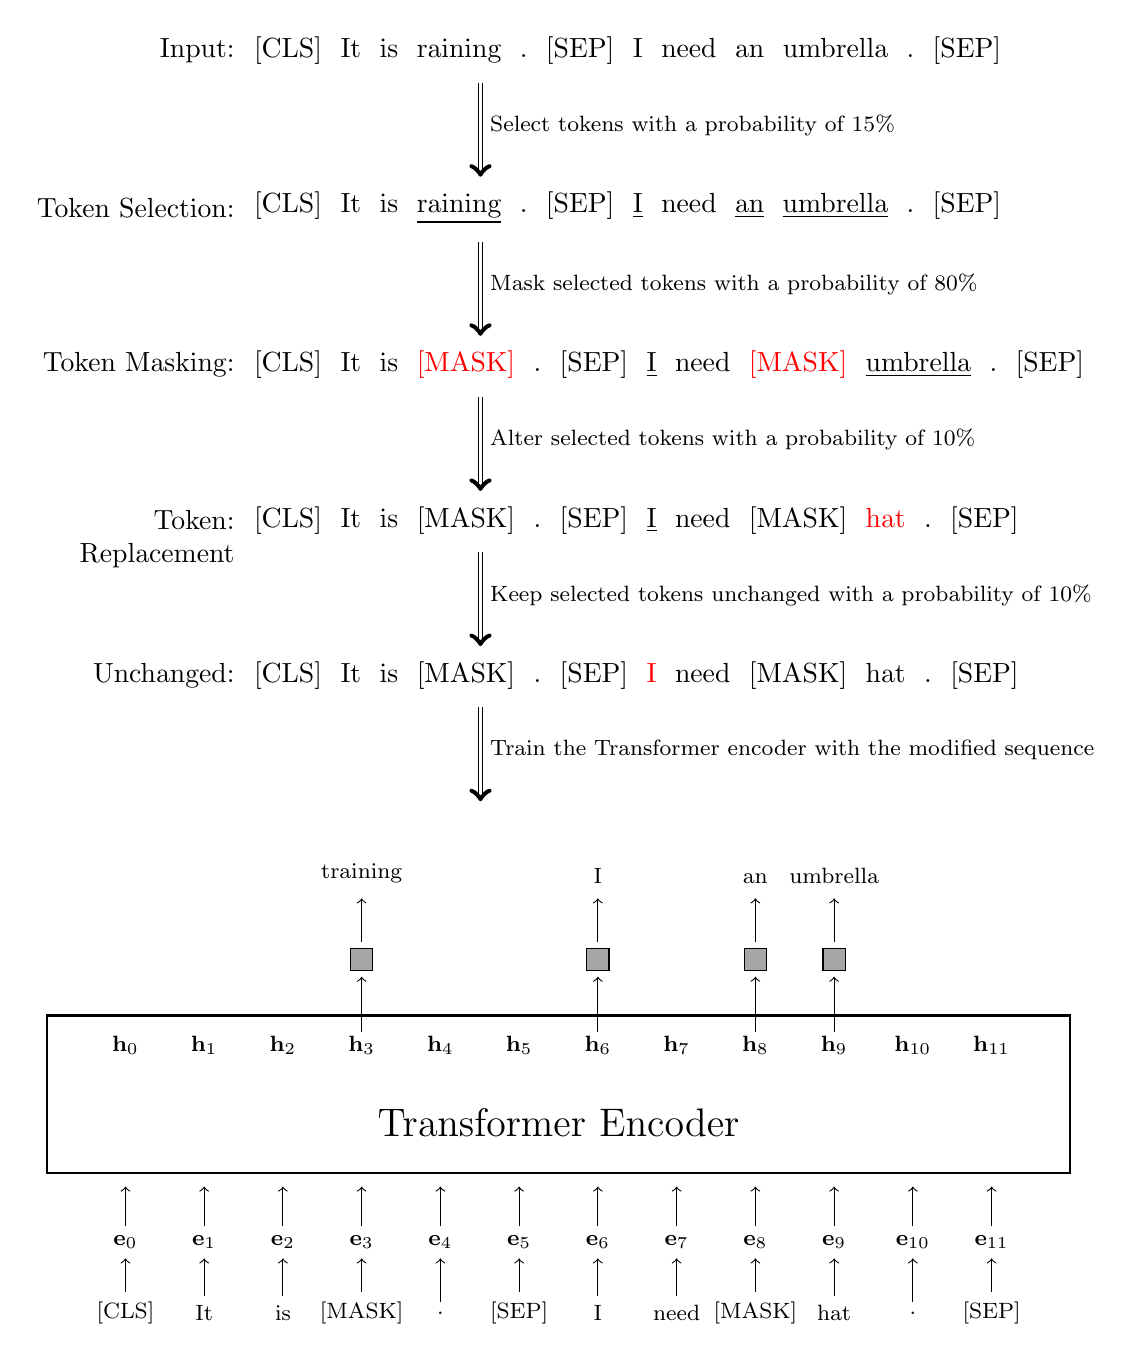
\begin{tikzpicture}
	
\def\vstep{1.3cm}
\def\ssep{1.0cm}

\tikzstyle{enode} = [minimum width=9*\nodestep,minimum height=1.4*\nodestep,inner sep=2pt,draw,thick];

\begin{scope}

%%%%%% input
\node [anchor=west] (original) at (0,0) {$[\mathrm{CLS}]$\ \ It\ \ is\ \ raining\ \ .\ \ $[\mathrm{SEP}]$\ \ I\ \ need\ \ an\ \ umbrella\ \ .\ \ $[\mathrm{SEP}]$};
\node [anchor=east] (originalcaption) at ([xshift=-0.0em]original.west) {Input:};

\draw [->,double,double distance=1pt] ([xshift=3cm,yshift=-3pt]original.south west) -- ([xshift=3cm,yshift=-\vstep]original.south west);
\node [anchor=west] (step0) at ([xshift=3cm,yshift=-0.5*\vstep]original.south west) {\footnotesize{Select tokens with a probability of $15\%$}};

%%%%%% selected tokens
\node [anchor=north west] (selected) at ([yshift=-\vstep-0.2em]original.south west) {$[\mathrm{CLS}]$\ \ It\ \ is\ \ \underline{raining}\ \ .\ \ $[\mathrm{SEP}]$\ \ \underline{I}\ \ need\ \ \underline{an}\ \ \underline{umbrella}\ \ .\ \ $[\mathrm{SEP}]$};
\node [anchor=east] (selectedcaption) at ([xshift=-0.0em]selected.west) {Token Selection:};

\draw [->,double,double distance=1pt] ([xshift=3cm,yshift=-3pt]selected.south west) -- ([xshift=3cm,yshift=-\vstep]selected.south west);
\node [anchor=west] (step1) at ([xshift=3cm,yshift=-0.5*\vstep]selected.south west) {\footnotesize{Mask selected tokens with a probability of $80\%$}};

%%%%%% masked tokens
\node [anchor=north west] (masked) at ([yshift=-\vstep-0.2em]selected.south west) {$[\mathrm{CLS}]$\ \ It\ \ is\ \ {\color{red} $\mathrm{[MASK]}$}\ \ .\ \ $[\mathrm{SEP}]$\ \ \underline{I}\ \ need\ \ {\color{red} $\mathrm{[MASK]}$}\ \ \underline{umbrella}\ \ .\ \ $[\mathrm{SEP}]$};
\node [anchor=east] (maskedcaption) at ([xshift=-0.0em]masked.west) {Token Masking:};

\draw [->,double,double distance=1pt] ([xshift=3cm,yshift=-3pt]masked.south west) -- ([xshift=3cm,yshift=-\vstep]masked.south west);
\node [anchor=west] (step2) at ([xshift=3cm,yshift=-0.5*\vstep]masked.south west) {\footnotesize{Alter selected tokens with a probability of $10\%$}};

%%%%%% replaced tokens
\node [anchor=north west] (replaced) at ([yshift=-\vstep-0.2em]masked.south west) {$[\mathrm{CLS}]$\ \ It\ \ is\ \ $\mathrm{[MASK]}$\ \ .\ \ $[\mathrm{SEP}]$\ \ \underline{I}\ \ need\ \ $\mathrm{[MASK]}$\ \ {\color{red} hat}\ \ .\ \ $[\mathrm{SEP}]$};
\node [anchor=east] (replacedcaption) at ([xshift=-0.0em]replaced.west) {Token:};
\node [anchor=north east] (replacedcaption2) at ([yshift=2pt]replacedcaption.south east) {Replacement};

\draw [->,double,double distance=1pt] ([xshift=3cm,yshift=-3pt]replaced.south west) -- ([xshift=3cm,yshift=-\vstep]replaced.south west);
\node [anchor=west] (step3) at ([xshift=3cm,yshift=-0.5*\vstep]replaced.south west) {\footnotesize{Keep selected tokens unchanged with a probability of $10\%$}};

%%%%%% unchanged tokens
\node [anchor=north west] (unchanged) at ([yshift=-\vstep-0.2em]replaced.south west) {$[\mathrm{CLS}]$\ \ It\ \ is\ \ $\mathrm{[MASK]}$\ \ .\ \ $[\mathrm{SEP}]$\ \ {\color{red} I}\ \ need\ \ $\mathrm{[MASK]}$\ \ hat\ \ .\ \ $[\mathrm{SEP}]$};
\node [anchor=east] (unchangedcaption) at ([xshift=-0.0em]unchanged.west) {Unchanged:};

\draw [->,double,double distance=1pt] ([xshift=3cm,yshift=-3pt]unchanged.south west) -- ([xshift=3cm,yshift=-\vstep]unchanged.south west);
\node [anchor=west] (step4) at ([xshift=3cm,yshift=-0.5*\vstep]unchanged.south west) {\footnotesize{Train the Transformer encoder with the modified sequence}};

%%%%%% train the encoder

\node [anchor=west] (w0) at ([yshift=-6*\vstep,xshift=-2cm]unchanged.south west) {\footnotesize{$[\mathrm{CLS}]$}};
\node [anchor=center] (w1) at ([xshift=\ssep]w0.center) {\footnotesize{It}};
\node [anchor=center] (w2) at ([xshift=\ssep]w1.center) {\footnotesize{is}};
\node [anchor=center] (w3) at ([xshift=\ssep]w2.center) {\footnotesize{$\mathrm{[MASK]}$}};
\node [anchor=center] (w4) at ([xshift=\ssep]w3.center) {\footnotesize{.}};
\node [anchor=center] (w5) at ([xshift=\ssep]w4.center) {\footnotesize{$\mathrm{[SEP]}$}};
\node [anchor=center] (w6) at ([xshift=\ssep]w5.center) {\footnotesize{I}};
\node [anchor=center] (w7) at ([xshift=\ssep]w6.center) {\footnotesize{need}};
\node [anchor=center] (w8) at ([xshift=\ssep]w7.center) {\footnotesize{$\mathrm{[MASK]}$}};
\node [anchor=center] (w9) at ([xshift=\ssep]w8.center) {\footnotesize{hat}};
\node [anchor=center] (w10) at ([xshift=\ssep]w9.center) {\footnotesize{.}};
\node [anchor=center] (w11) at ([xshift=\ssep]w10.center) {\footnotesize{$\mathrm{[SEP]}$}};

\node [anchor=center] (e0) at ([yshift=0.9*\ssep]w0.center) {\footnotesize{$\mathbf{e}_0$}};
\node [anchor=center] (e1) at ([yshift=0.9*\ssep]w1.center) {\footnotesize{$\mathbf{e}_1$}};
\node [anchor=center] (e2) at ([yshift=0.9*\ssep]w2.center) {\footnotesize{$\mathbf{e}_2$}};
\node [anchor=center] (e3) at ([yshift=0.9*\ssep]w3.center) {\footnotesize{$\mathbf{e}_3$}};
\node [anchor=center] (e4) at ([yshift=0.9*\ssep]w4.center) {\footnotesize{$\mathbf{e}_4$}};
\node [anchor=center] (e5) at ([yshift=0.9*\ssep]w5.center) {\footnotesize{$\mathbf{e}_5$}};
\node [anchor=center] (e6) at ([yshift=0.9*\ssep]w6.center) {\footnotesize{$\mathbf{e}_6$}};
\node [anchor=center] (e7) at ([yshift=0.9*\ssep]w7.center) {\footnotesize{$\mathbf{e}_7$}};
\node [anchor=center] (e8) at ([yshift=0.9*\ssep]w8.center) {\footnotesize{$\mathbf{e}_8$}};
\node [anchor=center] (e9) at ([yshift=0.9*\ssep]w9.center) {\footnotesize{$\mathbf{e}_9$}};
\node [anchor=center] (e10) at ([yshift=0.9*\ssep]w10.center) {\footnotesize{$\mathbf{e}_{10}$}};
\node [anchor=center] (e11) at ([yshift=0.9*\ssep]w11.center) {\footnotesize{$\mathbf{e}_{11}$}};

\draw [->] (w0.north) -- (e0.south);
\draw [->] (w1.north) -- (e1.south);
\draw [->] (w2.north) -- (e2.south);
\draw [->] (w3.north) -- (e3.south);
\draw [->] (w4.north) -- (e4.south);
\draw [->] (w5.north) -- (e5.south);
\draw [->] (w6.north) -- (e6.south);
\draw [->] (w7.north) -- (e7.south);
\draw [->] (w8.north) -- (e8.south);
\draw [->] (w9.north) -- (e9.south);
\draw [->] (w10.north) -- (e10.south);
\draw [->] (w11.north) -- (e11.south);

\draw [->] (e0.north) -- ([yshift=0.5*\ssep]e0.north);
\draw [->] (e1.north) -- ([yshift=0.5*\ssep]e1.north);
\draw [->] (e2.north) -- ([yshift=0.5*\ssep]e2.north);
\draw [->] (e3.north) -- ([yshift=0.5*\ssep]e3.north);
\draw [->] (e4.north) -- ([yshift=0.5*\ssep]e4.north);
\draw [->] (e5.north) -- ([yshift=0.5*\ssep]e5.north);
\draw [->] (e6.north) -- ([yshift=0.5*\ssep]e6.north);
\draw [->] (e7.north) -- ([yshift=0.5*\ssep]e7.north);
\draw [->] (e8.north) -- ([yshift=0.5*\ssep]e8.north);
\draw [->] (e9.north) -- ([yshift=0.5*\ssep]e9.north);
\draw [->] (e10.north) -- ([yshift=0.5*\ssep]e10.north);
\draw [->] (e11.north) -- ([yshift=0.5*\ssep]e11.north);

\node [anchor=south,minimum width=13*\ssep,minimum height=2*\ssep,draw,thick] (encoder) at ([yshift=1.5*\ssep,xshift=0.5*\ssep]w5.north) {};

\node [anchor=center] (h0) at ([yshift=3.4*\ssep]w0.center) {\footnotesize{$\mathbf{h}_0$}};
\node [anchor=center] (h1) at ([yshift=3.4*\ssep]w1.center) {\footnotesize{$\mathbf{h}_1$}};
\node [anchor=center] (h2) at ([yshift=3.4*\ssep]w2.center) {\footnotesize{$\mathbf{h}_2$}};
\node [anchor=center] (h3) at ([yshift=3.4*\ssep]w3.center) {\footnotesize{$\mathbf{h}_3$}};
\node [anchor=center] (h4) at ([yshift=3.4*\ssep]w4.center) {\footnotesize{$\mathbf{h}_4$}};
\node [anchor=center] (h5) at ([yshift=3.4*\ssep]w5.center) {\footnotesize{$\mathbf{h}_5$}};
\node [anchor=center] (h6) at ([yshift=3.4*\ssep]w6.center) {\footnotesize{$\mathbf{h}_6$}};
\node [anchor=center] (h7) at ([yshift=3.4*\ssep]w7.center) {\footnotesize{$\mathbf{h}_7$}};
\node [anchor=center] (h8) at ([yshift=3.4*\ssep]w8.center) {\footnotesize{$\mathbf{h}_8$}};
\node [anchor=center] (h9) at ([yshift=3.4*\ssep]w9.center) {\footnotesize{$\mathbf{h}_9$}};
\node [anchor=center] (h10) at ([yshift=3.4*\ssep]w10.center) {\footnotesize{$\mathbf{h}_{10}$}};
\node [anchor=center] (h11) at ([yshift=3.4*\ssep]w11.center) {\footnotesize{$\mathbf{h}_{11}$}};

\node [anchor=south,minimum height=0.8em,minimum width=0.8em,draw,fill=gray!70] (s3) at ([yshift=0.7*\ssep]h3.north) {};
\node [anchor=south,minimum height=0.8em,minimum width=0.8em,draw,fill=gray!70] (s6) at ([yshift=0.7*\ssep]h6.north) {};
\node [anchor=south,minimum height=0.8em,minimum width=0.8em,draw,fill=gray!70] (s8) at ([yshift=0.7*\ssep]h8.north) {};
\node [anchor=south,minimum height=0.8em,minimum width=0.8em,draw,fill=gray!70] (s9) at ([yshift=0.7*\ssep]h9.north) {};

\draw [->] ([yshift=-2pt]h3.north) -- ([yshift=-2pt]s3.south);
\draw [->] ([yshift=-2pt]h6.north) -- ([yshift=-2pt]s6.south);
\draw [->] ([yshift=-2pt]h8.north) -- ([yshift=-2pt]s8.south);
\draw [->] ([yshift=-2pt]h9.north) -- ([yshift=-2pt]s9.south);

\node [anchor=south] (o3) at ([yshift=0.7*\ssep]s3.north) {\footnotesize{training}};
\node [anchor=south] (o6) at ([yshift=0.7*\ssep]s6.north) {\footnotesize{I}};
\node [anchor=south] (o8) at ([yshift=0.7*\ssep,xshift=0.0em]s8.north) {\footnotesize{an}};
\node [anchor=south] (o9) at ([yshift=0.7*\ssep,xshift=0.0em]s9.north) {\footnotesize{umbrella}};

\draw [->] ([yshift=2pt]s3.north) -- ([yshift=0.7*\ssep-2pt]s3.north);
\draw [->] ([yshift=2pt]s6.north) -- ([yshift=0.7*\ssep-2pt]s6.north);
\draw [->] ([yshift=2pt]s8.north) -- ([yshift=0.7*\ssep-2pt]s8.north);
\draw [->] ([yshift=2pt]s9.north) -- ([yshift=0.7*\ssep-2pt]s9.north);

\node [anchor=south] (encodercaption) at ([yshift=1em]encoder.south) {\Large{Transformer Encoder}};

\end{scope}
	
\end{tikzpicture}

\caption{A running example of BERT-style masked language modeling. First, $15\%$ of the tokens are randomly selected. These selected tokens are then processed in one of three ways: replaced with a $\mathrm{[MASK]}$ token ($80\%$ of the time), replaced with a random token ($10\%$ of the time), or kept unchanged ($10\%$ of the time). The model is trained to predict these selected tokens based on the modified sequence. $\mathbf{e}_i$ represents the embedding of the token at the position $i$. Gray boxes represent the Softmax layers.}
\label{fig:example-bert-mlm-loss}
\end{figure}

For next sentence prediction, we follow the method described in Section~\ref{sec:pre-training-as-classification}. Each training sample is assigned a label from the set $\{\mathrm{IsNext}, \mathrm{NotNext}\}$, for example,
\begin{eqnarray}
\textrm{Sequence:} & & \textrm{$[\mathrm{CLS}]$ It is raining . $[\mathrm{SEP}]$ I need an umbrella . $[\mathrm{SEP}]$} \nonumber \\
\textrm{Label:} & & \textrm{$\mathrm{IsNext}$} \nonumber \\
& & \nonumber \\
\textrm{Sequence:} & & \textrm{$[\mathrm{CLS}]$ The cat sleeps on the windowsill . $[\mathrm{SEP}]$ Apples grow on trees . $[\mathrm{SEP}]$} \nonumber \\
\textrm{Label:} & & \textrm{$\mathrm{NotNext}$} \nonumber
\end{eqnarray}

\noindent The output vector of the encoder for the first token $\mathrm{[CLS]}$ is viewed as the sequence representation, denoted by $\mathbf{h}_{\mathrm{cls}}$ (or $\mathbf{h}_0$). A classifier is built on top of $\mathbf{h}_{\mathrm{cls}}$. Then, we can compute the probability of a label $c$ given $\mathbf{h}_{\mathrm{cls}}$, i.e., $\Pr(c|\mathbf{h}_{\mathrm{cls}})$. There are many loss functions one can choose for classification problems. For example, in maximum likelihood training, we can define $\mathrm{Loss}_{\mathrm{nsp}}$ as
\begin{eqnarray}
\mathrm{Loss}_{\mathrm{nsp}} & = & -\log \Pr(c_{\mathrm{gold}}|\mathbf{h}_{\mathrm{cls}}),
\end{eqnarray}

\noindent where $c_{\mathrm{gold}}$ is the correct label for this sample.

\subsubsection{Model Setup}

\noindent As shown in Figure~\ref{fig:bert-architecture}, BERT models are based on the standard Transformer encoder architecture. The input is a sequence of embeddings, each of which is the sum of the token embedding, the positional embedding, and the segment embedding.
\begin{eqnarray}
\mathbf{e} & = & \mathbf{x} + \mathbf{e}_{\mathrm{pos}} + \mathbf{e}_{\mathrm{seg}}.
\end{eqnarray}

\noindent Both the token embedding ($\mathbf{x}$) and the positional embedding ($\mathbf{e}_{\mathrm{pos}}$) are identical to those used in the original Transformer. The segment embedding ($\mathbf{e}_{\mathrm{seg}}$) is a new addition that indicates whether a token belongs to $\mathrm{Sent}_{A}$ or $\mathrm{Sent}_{B}$. This is illustrated by the following example:

\vspace{0.5em}
\begin{center}
\begingroup
\renewcommand{\arraystretch}{1.2}
\setlength{\tabcolsep}{2pt}
{\small
\makebox[\textwidth]{
\begin{tabular}{r | c c c c c c c c c c c c}
Token & $[\mathrm{CLS}]$ & It & is & raining & . & $[\mathrm{SEP}]$ & I & need & an & umbrella & . & $[\mathrm{SEP}]$ \\ \hline
$\mathbf{x}$ & $\mathbf{x}_{0}$ & $\mathbf{x}_{1}$ & $\mathbf{x}_{2}$ & $\mathbf{x}_{3}$ & $\mathbf{x}_{4}$ & $\mathbf{x}_{5}$ & $\mathbf{x}_{6}$ & $\mathbf{x}_{7}$ & $\mathbf{x}_{8}$ & $\mathbf{x}_{9}$ & $\mathbf{x}_{10}$ & $\mathbf{x}_{11}$ \\
$\mathbf{e}_{\mathrm{pos}}$ & \footnotesize{$\mathrm{PE}(0)$} & \footnotesize{$\mathrm{PE}(1)$} & \footnotesize{$\mathrm{PE}(2)$} & \footnotesize{$\mathrm{PE}(3)$} & \footnotesize{$\mathrm{PE}(4)$} & \footnotesize{$\mathrm{PE}(5)$} & \footnotesize{$\mathrm{PE}(6)$} & \footnotesize{$\mathrm{PE}(7)$} & \footnotesize{$\mathrm{PE}(8)$} & \footnotesize{$\mathrm{PE}(9)$} & \footnotesize{$\mathrm{PE}(10)$} & \footnotesize{$\mathrm{PE}(11)$} \\
$\mathbf{e}_{\mathrm{seg}}$ & $\mathbf{e}_{A}$ & $\mathbf{e}_{A}$ & $\mathbf{e}_{A}$ & $\mathbf{e}_{A}$ & $\mathbf{e}_{A}$ & $\mathbf{e}_{A}$ & $\mathbf{e}_{B}$ & $\mathbf{e}_{B}$ & $\mathbf{e}_{B}$ & $\mathbf{e}_{B}$ & $\mathbf{e}_{B}$ & $\mathbf{e}_{B}$
\end{tabular}
}
}
\endgroup
\end{center}
\vspace{0.5em}

\begin{figure}[!t]
\centering
% !Mode:: "TeX:UTF-8"
% !TEX encoding = UTF-8 Unicode

\begin{tikzpicture}
	
\def\nsize{4.5cm}
\def\vstep{1cm}

\tikzstyle{enode} = [minimum width=\nsize,minimum height=0.18*\nsize,inner sep=2pt,draw,thick];

\begin{scope}

\node [enode,anchor=west,draw] (selfattention) at (0,0) {Self-attention};

\node [anchor=north,minimum width=0.33*\nsize,minimum height=0.33*0.4*\nsize,draw] (posembedding) at ([yshift=-1.2*\vstep]selfattention.south) {\small{Position}};
\node [anchor=east,minimum width=0.33*\nsize,minimum height=0.33*0.4*\nsize,draw] (tokenembedding) at ([xshift=-0pt]posembedding.west) {\small{Token}};
\node [anchor=west,minimum width=0.33*\nsize,minimum height=0.33*0.4*\nsize,draw] (segembedding) at ([xshift=-0pt]posembedding.east) {\small{Segment}};

\node [anchor=north] (input) at ([yshift=-\vstep]posembedding.south) {$x_{0} x_{1} ... x_{m}$};

\draw [->,thick] ([yshift=0pt]input.north) -- ([yshift=-2pt]posembedding.south);
\draw [->,thick] ([yshift=2pt]posembedding.north) -- ([yshift=-2pt]selfattention.south);

\node [enode,anchor=south,draw] (lnormself) at ([yshift=0.8*\vstep]selfattention.north) {Layer Normalization};
\node [enode,anchor=south,draw] (ffn) at ([yshift=1.4*\vstep]lnormself.north) {FFN};
\node [enode,anchor=south,draw] (lnormffn) at ([yshift=0.8*\vstep]ffn.north) {Layer Normalization};

\draw [->,thick] ([yshift=2pt]selfattention.north) -- ([yshift=-2pt]lnormself.south);
\draw [->,thick] ([yshift=2pt]lnormself.north) -- ([yshift=-2pt]ffn.south);
\draw [->,thick] ([yshift=2pt]ffn.north) -- ([yshift=-2pt]lnormffn.south);

\draw [->,thick] ([yshift=-1em,xshift=-2pt]selfattention.south) -- ([yshift=-1em,xshift=-1em]selfattention.south west) -- ([xshift=-1em]lnormself.west) -- ([xshift=-2pt]lnormself.west);
\draw [->,thick] ([yshift=-1em,xshift=-2pt]ffn.south) -- ([yshift=-1em,xshift=-1em]ffn.south west) -- ([xshift=-1em]lnormffn.west) -- ([xshift=-2pt]lnormffn.west);

\node [enode,anchor=south,draw] (outputlayer) at ([yshift=1.2*\vstep]lnormffn.north) {Output Layer};
\node [anchor=south] (output) at ([yshift=\vstep]outputlayer.north) {$...$};

\draw [->,thick] ([yshift=2pt]lnormffn.north) -- ([yshift=-2pt]outputlayer.south);
\draw [->,thick] ([yshift=2pt]outputlayer.north) -- ([yshift=-2pt]output.south);

\node [anchor=west] (encoderoutput) at ([yshift=0.7*\vstep]lnormffn.north) {$\mathbf{h}_0 \mathbf{h}_1 ... \mathbf{h}_m$};

\begin{pgfonlayer}{background}
\node [anchor=south,densely dashed,minimum width=1.30*\nsize,minimum height=0.75*\nsize,draw]  (selfattention-sub-layer) at ([yshift=-0.6cm]selfattention.south) {};
\node [anchor=south,densely dashed,minimum width=1.30*\nsize,minimum height=0.75*\nsize,draw]  (ffn-sub-layer) at ([yshift=-0.6cm]ffn.south) {};

\draw [decoration={brace,amplitude=5pt},decorate] ([xshift=-0.7em,yshift=-2pt]selfattention-sub-layer.south west) -- ([xshift=-0.7em,yshift=2pt]ffn-sub-layer.north west) node [pos=0.5,left,xshift=-0.6em] (timeslayer) {};
\end{pgfonlayer}
\node [anchor=north east] (timeslayer2) at (timeslayer.south east) {layers};

\node [anchor=west] (vocabulary) at ([xshift=1.5cm,yshift=-0.8cm]segembedding.east) {Input};
\node [anchor=north west] (vocabulary2) at ([yshift=0.4em]vocabulary.south west) {$x_i$ is the $i$-th token in the input};
\node [anchor=north west] (vocabulary3) at ([yshift=0.3em]vocabulary2.south west) {and corresponds to an entry in $V$};

\node [anchor=west] (embeddingcaption) at ([xshift=1.5cm,yshift=1.0cm]segembedding.east) {Embedding};
\node [anchor=north west] (embeddingcaption2) at ([yshift=0.2em]embeddingcaption.south west) {$\mathbf{e} = \mathbf{x} + \mathbf{e}_{\mathrm{pos}} + \mathbf{e}_{\mathrm{seg}} \in \mathbb{R}^{d_e}$};

\node [anchor=west] (selfattentioncaption) at ([xshift=1.5cm,yshift=1.2cm]selfattention.east) {Self-attention Sub-layer};
\node [anchor=north west] (selfattentioncaption2) at ([yshift=0.4em]selfattentioncaption.south west) {hidden size: $d$};
\node [anchor=north west] (selfattentioncaption3) at ([yshift=0.3em]selfattentioncaption2.south west) {number of heads: $n_{\mathrm{head}}$};

\node [anchor=west] (ffncaption) at ([xshift=1.5cm,yshift=1.2cm]ffn.east) {FFN Sub-layer};
\node [anchor=north west] (ffncaption2) at ([yshift=0.4em]ffncaption.south west) {hidden size: $d$};
\node [anchor=north west] (ffncaption3) at ([yshift=0.3em]ffncaption2.south west) {FFN hidden size: $d_{\mathrm{ffn}}$};

\node [anchor=west] (eoutputcaption) at ([xshift=1.5cm,yshift=2.0cm]lnormffn.east) {Encoder Output};
\node [anchor=north west] (eoutputcaption2) at ([yshift=0.3em]eoutputcaption.south west) {$\mathbf{h}_i \in \mathbb{R}^{d}$ is the contextual};
\node [anchor=north west] (eoutputcaption3) at ([yshift=0.3em]eoutputcaption2.south west) {representation of $x_i$};

\draw [-,thin] ([xshift=2pt]input.east) -- ([xshift=-2pt]vocabulary.west);
\draw [-,thin] ([xshift=2pt]segembedding.east) -- ([xshift=-2pt]embeddingcaption.west);
\draw [-,thin] ([xshift=2pt]selfattention-sub-layer.east) -- ([xshift=-2pt]selfattentioncaption.west);
\draw [-,thin] ([xshift=2pt]ffn-sub-layer.east) -- ([xshift=-2pt]ffncaption.west);
\draw [-,thin] ([xshift=2pt]encoderoutput.east) -- ([xshift=-2pt]eoutputcaption.west);

\end{scope}
	
\end{tikzpicture}

\caption{The model architecture of BERT (Transformer encoder). The input tokens are first represented as embeddings, each of which is the sum of the corresponding token embedding, positional embedding, and segment embedding. Then, the embedding sequence is processed by a stack of Transformer layers. Each layer in this stack includes a self-attention sub-layer and an FFN sub-layer. The output of the BERT model is a sequence of vectors produced by the final Transformer layer.}
\label{fig:bert-architecture}
\end{figure}

The main part of BERT models is a multi-layer Transformer network. A Transformer layer consists of a self-attention sub-layer and an FFN sub-layer. Both sub-layers follow the post-norm architecture: $\mathrm{output} = \mathrm{LNorm}(F(\mathrm{input}) + \mathrm{input})$, where $F(\cdot)$ is the core function of the sub-layer (either a self-attention model or an FFN), and $\mathrm{LNorm}(\cdot)$ is the layer normalization unit. Typically, a number of Transformer layers are stacked to form a deep network. For each position in the sequence, the final output representation is the real-valued vector produced by the uppermost layer.

There are several aspects one may consider in developing BERT models.

\begin{itemize}
\item \vspace{0.5em} \textbf{Vocabulary Size} ($|V|$). In Transformers, each token corresponds to an entry in a vocabulary $V$. Large vocabularies can cover more surface form variants of words, but may lead to increased storage requirements.
\item \vspace{0.3em} \textbf{Embedding Size} ($d_e$). Every token is represented as a $d_e$-dimensional real-valued vector. As presented above, this vector is the sum of the token embedding, positional embedding, and segment embedding, all of which are also $d_e$-dimensional real-valued vectors.
\item \vspace{0.3em} \textbf{Hidden Size} ($d$). The input and output of a sub-layer are of $d$ dimensions. Besides, most of the hidden states of a sub-layer are $d$-dimensional vectors. In general, $d$ can be roughly viewed as the width of the network.
\item \vspace{0.3em} \textbf{Number of Heads} ($n_{\mathrm{head}}$). In self-attention sub-layers, one needs to specify the number of heads used in multi-head self-attention. A larger number of heads allows the model to jointly attend to information from a greater number of representation subspaces. In practical systems, we often set $n_{\mathrm{head}} \ge 4$.
\item \vspace{0.3em} \textbf{FFN Hidden Size} ($d_{\textrm{ffn}}$). The size of the hidden layer of the FFNs used in Transformers is typically larger than $d$. For example, a typical setting is $d_{\textrm{ffn}} = 4 d$. For larger Transformers, such as recent large models, $d_{\textrm{ffn}}$ may be set to a very large value.
\item \vspace{0.3em} \textbf{Model Depth} ($L$). Using deep networks is an effective way to improve the expressive power of Transformers. For BERT models, $L$ is typically set to $12$ or $24$. However, networks with even greater depth are also feasible and can be applied for further enhancements.
\end{itemize}
\vspace{0.5em}

Different settings of these hyper-parameters lead to different model sizes. Two widely used configurations are BERT$_{\mathrm{base}}$ and BERT$_{\mathrm{large}}$:

\begin{itemize}
\item \vspace{0.5em} BERT$_{\mathrm{base}}$: $d=768$, $L=12$, $n_{\mathrm{head}}=12$, total number of parameters $=110$M.
\item \vspace{0.3em} BERT$_{\mathrm{large}}$: $d=1,024$, $L=24$, $n_{\mathrm{head}}=16$, total number of parameters $=340$M.
\end{itemize}
\vspace{0.3em}

The training of BERT models follows the standard procedure for Transformers. Training larger models such as BERT$_{\mathrm{large}}$ requires more training effort and time. This is a common problem for pre-training, especially when a model is trained on a very large amount of data. In practice, training efficiency is often a major concern. A common practice is to first train a BERT model on relatively short sequences for a large number of training steps, and then continue training it on full-length sequences for the remaining training steps.

\subsection{More Training and Larger Models}

\noindent BERT is a milestone in NLP and has sparked extensive subsequent work. One direction is to scale up pre-training, which generally involves two approaches: increasing the amount of training data and increasing the number of model parameters.

\mindex{RoBERTa}, an extension of the standard BERT model, is an example of such efforts~\cite{liu-etal:2019roberta}. It introduces two major improvements. First, simply using more training data and more compute can improve BERT models without the need to change the model architecture. Second, removing the NSP loss does not degrade performance on downstream tasks if the training is scaled up. These findings suggest exploring a general direction of pre-training: we can continue to improve pre-training by scaling it up on simple pre-training tasks.

A second approach to improving BERT models is to increase the number of model parameters. For example, in \citet{he-etal:2021deberta}'s work, a 1.5 billion-parameter BERT-like model is built by increasing both the model depth and hidden size. However, scaling up BERT and various other pre-trained models introduces new challenges in training, for example, training very large models often becomes unstable and difficult to converge. This makes the problem more complicated, and requires careful consideration of various aspects, such as model architecture, parallel computation, and parameter initialization. In another example, \citet{shoeybi-etal:2019megatron} successfully trained a 3.9 billion-parameter BERT-like model, where hundreds of GPUs were used to manage the increased computational demands.

\subsection{More Efficient Models}

\noindent Compared to its predecessors, BERT is a relatively large model for the time it was proposed. This increase in model size results in larger memory requirements and slower inference. Developing smaller and faster BERT models is part of the broader challenge of building efficient Transformers, which has been extensively discussed in the literature \cite{Tay-etal:2020efficient,xiao-and-zhu:2023introduction}. However, a deeper exploration of this topic is beyond the scope of this section. Here, we instead focus on a few efficient variants of BERT.

Several research threads are of particular interest for developing efficient BERT models. First, work on knowledge distillation, such as training a student model using the outputs of a well-trained teacher model, demonstrates that more compact models can be obtained by transferring knowledge from larger ones. Given that BERT models are multi-layer networks with several different types of layers, knowledge distillation can be applied at different levels of representation. For example, beyond distilling knowledge from the output layers, it is also possible to incorporate a training loss that measures the difference between the outputs of hidden layers for the teacher and student models~\cite{sun2020-etal:mobilebert,jiao-etal:2020tinybert}. Indeed, knowledge distillation has been one of the most widely used techniques for learning small pre-trained models.

Second, conventional model compression methods can be directly applied to BERT. One common approach is to apply general-purpose pruning methods to Transformer encoders~\cite{gale-etal:2019state}. This generally involves removing entire layers~\cite{fan-etal:2019reducing} or a certain percentage of parameters in the networks~\cite{sanh-etal:2020movement,chen-etal:2020lottery}. Pruning is also applicable to multi-head attention models. For example, \citet{michel-etal:2019sixteen} show that removing some of the heads does not significantly degrade performance of BERT models, but speeds up the inference of these models. Another approach to compressing BERT models is quantization~\cite{shen-etal:2020qbert}. By representing model parameters as low-precision numbers, we can compress the models greatly. While this method is not specific to BERT models, it proves effective for large Transformer-based architectures.

Third, considering that BERT models are relatively deep and large networks, another thread of research uses dynamic networks to adapt these models for efficient inference. An idea in this paradigm is to dynamically choose the layers for processing a token, for example, in depth-adaptive models we exit at some optimal depth and thus skip the rest of the layers in the layer stack~\cite{xin-etal:2020deebert,zhou-etal:2020bert}. Similarly, we can develop length-adaptive models in which the length of the input sequence is dynamically adjusted. For example, we can skip some of the tokens in the input sequence so that the model can reduce computational load on less important tokens, enhancing overall efficiency.

Fourth, it is also possible to share parameters across layers to reduce the size of BERT models. A simple way to do this is to share the parameters of a whole Transformer layer across the layer stack~\cite{dehghani-etal:2018universal,lan-etal:2020albert}. In addition to the reduced number of parameters, this enables reuse of the same layer in a multi-layer Transformer network, leading to savings of memory footprint at test time.

\subsection{Multilingual Models}

\noindent The initial BERT model was primarily focused on English. Soon after this model was proposed, it was extended to many languages. One simple way to do this is to develop a separate model for each language. Another approach, which has become more popular in recent work on large language models, is to train multilingual models directly on data from all the languages. Accordingly, \mindex{multilingual BERT} (\mindexraw{mBERT}) models were developed by training on text from 104 languages \footnote{\url{https://github.com/google-research/bert/}}. The primary difference from monolingual BERT models is that mBERT models use larger vocabularies to cover tokens from multiple languages. As a result, the representations of tokens from different languages are mapped into the same space, allowing for the sharing of knowledge across languages.

One of the most important applications of multilingual pre-trained models is cross-lingual transfer learning. In a zero-shot cross-lingual setting, a model is fine-tuned on a task using data from a source language and then applied to the same task in a target language without any target-language training data. In cross-lingual text classification, for example, we can fine-tune a multilingual pre-trained model on annotated English documents and then directly use the fine-tuned model to classify Chinese documents.

An improvement to multilingual pre-trained models like mBERT is to introduce bilingual data into pre-training. Rather than training solely on monolingual data from multiple languages, bilingual training explicitly models the relationship between tokens in two languages. The resulting model will have cross-lingual transfer abilities, and thus can be easily adapted to different languages. \citet{lample-conneau:2019cross} propose an approach to pre-training \mindex{cross-lingual language models} (\mindex{XLMs}). In their work, a cross-lingual language model can be trained using either causal language modeling or masked language modeling. For masked language modeling pre-training, the model is treated as an encoder. The training objective is the same as BERT: we maximize the probabilities of some randomly selected tokens which are either masked, replaced with random tokens, or kept unchanged in the input. If we consider bilingual data in pre-training, we sample a pair of aligned sentences each time. Then, the two sentences are packed together to form a single sequence used for training. For example, consider an English-Chinese sentence pair

\vspace{0.5em}
\begin{center}
\begin{CJK*}{UTF8}{gbsn}鲸鱼\ \ 是\ \ 哺乳\ \ 动物\ \ 。\end{CJK*}\ \ \ $\leftrightarrow$\ \ \ Whales are mammals\ \ .
\end{center}
\vspace{0.5em}

\noindent We can pack them to obtain a sequence, like this

\vspace{0.5em}
\begin{center}
$\mathrm{[CLS]}$ \begin{CJK*}{UTF8}{gbsn}鲸鱼\ \ 是\ \ 哺乳\ \ 动物\ \ 。\end{CJK*}\ \ $\mathrm{[SEP]}$ \ \ Whales are mammals\ \ .\ \ $\mathrm{[SEP]}$
\end{center}
\vspace{0.5em}

\noindent We then select a certain percentage of the tokens and replace them with $\mathrm{[MASK]}$.

\vspace{0.5em}
\begin{center}
$\mathrm{[CLS]}$ \begin{CJK*}{UTF8}{gbsn}$\mathrm{[MASK]}$\ \ 是\ \ $\mathrm{[MASK]}$\ \ 动物\ \ 。\end{CJK*}\ \ $\mathrm{[SEP]}$ \ \ Whales $\mathrm{[MASK]}$ $\mathrm{[MASK]}$\ \ .\ \ $\mathrm{[SEP]}$
\end{center}
\vspace{0.5em}

\noindent The goal of pre-training is to maximize the product of the probabilities of the masked tokens given the above sequence. By performing training in this way, the model can learn to represent both the English and Chinese sequences, as well as to capture the correspondences between tokens in the two languages. For example, predicting the Chinese token \begin{CJK*}{UTF8}{gbsn} 鲸鱼\end{CJK*} may require the information from the English token \textit{Whales}. Aligning the representations of the two languages essentially transforms the model into a ``translation'' model. This training objective is therefore also called \mindex{translation language modeling}. Figure~\ref{fig:translation-language-modeling} shows an illustration of this approach.

\begin{figure}[!t]
\centering
% !Mode:: "TeX:UTF-8"
% !TEX encoding = UTF-8 Unicode

\begin{tikzpicture}
	
\def\vstep{1.3cm}
\def\ssep{1.0cm}

\tikzstyle{enode} = [minimum width=9*\nodestep,minimum height=1.4*\nodestep,inner sep=2pt,draw,thick];

\begin{scope}

%%%%%% train the encoder

\node [anchor=west] (w0) at (0,0) {\footnotesize{$[\mathrm{CLS}]$}};
\node [anchor=center] (w1) at ([xshift=\ssep]w0.center) {\tiny{{\color{blue} $[\mathrm{MASK}]$}}};
\node [anchor=center] (w2) at ([xshift=\ssep]w1.center) {\footnotesize{\begin{CJK*}{UTF8}{gbsn}是\end{CJK*}}};
\node [anchor=center] (w3) at ([xshift=\ssep]w2.center) {\tiny{{\color{blue} $[\mathrm{MASK}]$}}};
\node [anchor=center] (w4) at ([xshift=\ssep]w3.center) {\footnotesize{\begin{CJK*}{UTF8}{gbsn}动物\end{CJK*}}};
\node [anchor=center] (w5) at ([xshift=\ssep]w4.center) {\footnotesize{\begin{CJK*}{UTF8}{gbsn}。\end{CJK*}}};
\node [anchor=center] (w6) at ([xshift=\ssep]w5.center) {\footnotesize{$\mathrm{[SEP]}$}};
\node [anchor=center] (w7) at ([xshift=\ssep]w6.center) {\footnotesize{Whales}};
\node [anchor=center] (w8) at ([xshift=\ssep]w7.center) {\tiny{{\color{blue} $[\mathrm{MASK}]$}}};
\node [anchor=center] (w9) at ([xshift=\ssep]w8.center) {\tiny{{\color{blue} $[\mathrm{MASK}]$}}};
\node [anchor=center] (w10) at ([xshift=\ssep]w9.center) {\footnotesize{.}};
\node [anchor=center] (w11) at ([xshift=\ssep]w10.center) {\footnotesize{$\mathrm{[SEP]}$}};

\node [anchor=north] (l0) at ([yshift=-0.2cm]w0.center) {\scriptsize{(zh)}};
\node [anchor=north] (l1) at ([yshift=-0.2cm]w1.center) {\scriptsize{(zh)}};
\node [anchor=north] (l2) at ([yshift=-0.2cm]w2.center) {\scriptsize{(zh)}};
\node [anchor=north] (l3) at ([yshift=-0.2cm]w3.center) {\scriptsize{(zh)}};
\node [anchor=north] (l4) at ([yshift=-0.2cm]w4.center) {\scriptsize{(zh)}};
\node [anchor=north] (l5) at ([yshift=-0.2cm]w5.center) {\scriptsize{(zh)}};
\node [anchor=north] (l6) at ([yshift=-0.2cm]w6.center) {\scriptsize{(zh)}};
\node [anchor=north] (l7) at ([yshift=-0.2cm]w7.center) {\scriptsize{(en)}};
\node [anchor=north] (l8) at ([yshift=-0.2cm]w8.center) {\scriptsize{(en)}};
\node [anchor=north] (l9) at ([yshift=-0.2cm]w9.center) {\scriptsize{(en)}};
\node [anchor=north] (l10) at ([yshift=-0.2cm]w10.center) {\scriptsize{(en)}};
\node [anchor=north] (l11) at ([yshift=-0.2cm]w11.center) {\scriptsize{(en)}};

\node [anchor=center] (e0) at ([yshift=0.9*\ssep]w0.center) {\footnotesize{$\mathbf{e}_0$}};
\node [anchor=center] (e1) at ([yshift=0.9*\ssep]w1.center) {\footnotesize{$\mathbf{e}_1$}};
\node [anchor=center] (e2) at ([yshift=0.9*\ssep]w2.center) {\footnotesize{$\mathbf{e}_2$}};
\node [anchor=center] (e3) at ([yshift=0.9*\ssep]w3.center) {\footnotesize{$\mathbf{e}_3$}};
\node [anchor=center] (e4) at ([yshift=0.9*\ssep]w4.center) {\footnotesize{$\mathbf{e}_4$}};
\node [anchor=center] (e5) at ([yshift=0.9*\ssep]w5.center) {\footnotesize{$\mathbf{e}_5$}};
\node [anchor=center] (e6) at ([yshift=0.9*\ssep]w6.center) {\footnotesize{$\mathbf{e}_6$}};
\node [anchor=center] (e7) at ([yshift=0.9*\ssep]w7.center) {\footnotesize{$\mathbf{e}_7$}};
\node [anchor=center] (e8) at ([yshift=0.9*\ssep]w8.center) {\footnotesize{$\mathbf{e}_8$}};
\node [anchor=center] (e9) at ([yshift=0.9*\ssep]w9.center) {\footnotesize{$\mathbf{e}_9$}};
\node [anchor=center] (e10) at ([yshift=0.9*\ssep]w10.center) {\footnotesize{$\mathbf{e}_{10}$}};
\node [anchor=center] (e11) at ([yshift=0.9*\ssep]w11.center) {\footnotesize{$\mathbf{e}_{11}$}};

\draw [->] (w0.north) -- (e0.south);
\draw [->] (w1.north) -- (e1.south);
\draw [->] (w2.north) -- (e2.south);
\draw [->] (w3.north) -- (e3.south);
\draw [->] (w4.north) -- (e4.south);
\draw [->] (w5.north) -- (e5.south);
\draw [->] (w6.north) -- (e6.south);
\draw [->] (w7.north) -- (e7.south);
\draw [->] (w8.north) -- (e8.south);
\draw [->] (w9.north) -- (e9.south);
\draw [->] (w10.north) -- (e10.south);
\draw [->] (w11.north) -- (e11.south);

\draw [->] (e0.north) -- ([yshift=0.5*\ssep]e0.north);
\draw [->] (e1.north) -- ([yshift=0.5*\ssep]e1.north);
\draw [->] (e2.north) -- ([yshift=0.5*\ssep]e2.north);
\draw [->] (e3.north) -- ([yshift=0.5*\ssep]e3.north);
\draw [->] (e4.north) -- ([yshift=0.5*\ssep]e4.north);
\draw [->] (e5.north) -- ([yshift=0.5*\ssep]e5.north);
\draw [->] (e6.north) -- ([yshift=0.5*\ssep]e6.north);
\draw [->] (e7.north) -- ([yshift=0.5*\ssep]e7.north);
\draw [->] (e8.north) -- ([yshift=0.5*\ssep]e8.north);
\draw [->] (e9.north) -- ([yshift=0.5*\ssep]e9.north);
\draw [->] (e10.north) -- ([yshift=0.5*\ssep]e10.north);
\draw [->] (e11.north) -- ([yshift=0.5*\ssep]e11.north);

\node [anchor=south,minimum width=13*\ssep,minimum height=2*\ssep,draw,thick] (encoder) at ([yshift=1.5*\ssep,xshift=0.5*\ssep]w5.north) {};

\node [anchor=center] (h0) at ([yshift=3.4*\ssep]w0.center) {\footnotesize{$\mathbf{h}_0$}};
\node [anchor=center] (h1) at ([yshift=3.4*\ssep]w1.center) {\footnotesize{$\mathbf{h}_1$}};
\node [anchor=center] (h2) at ([yshift=3.4*\ssep]w2.center) {\footnotesize{$\mathbf{h}_2$}};
\node [anchor=center] (h3) at ([yshift=3.4*\ssep]w3.center) {\footnotesize{$\mathbf{h}_3$}};
\node [anchor=center] (h4) at ([yshift=3.4*\ssep]w4.center) {\footnotesize{$\mathbf{h}_4$}};
\node [anchor=center] (h5) at ([yshift=3.4*\ssep]w5.center) {\footnotesize{$\mathbf{h}_5$}};
\node [anchor=center] (h6) at ([yshift=3.4*\ssep]w6.center) {\footnotesize{$\mathbf{h}_6$}};
\node [anchor=center] (h7) at ([yshift=3.4*\ssep]w7.center) {\footnotesize{$\mathbf{h}_7$}};
\node [anchor=center] (h8) at ([yshift=3.4*\ssep]w8.center) {\footnotesize{$\mathbf{h}_8$}};
\node [anchor=center] (h9) at ([yshift=3.4*\ssep]w9.center) {\footnotesize{$\mathbf{h}_9$}};
\node [anchor=center] (h10) at ([yshift=3.4*\ssep]w10.center) {\footnotesize{$\mathbf{h}_{10}$}};
\node [anchor=center] (h11) at ([yshift=3.4*\ssep]w11.center) {\footnotesize{$\mathbf{h}_{11}$}};

\node [anchor=south,minimum height=0.8em,minimum width=0.8em,draw,fill=gray!70] (s1) at ([yshift=0.7*\ssep]h1.north) {};
\node [anchor=south,minimum height=0.8em,minimum width=0.8em,draw,fill=gray!70] (s3) at ([yshift=0.7*\ssep]h3.north) {};
\node [anchor=south,minimum height=0.8em,minimum width=0.8em,draw,fill=gray!70] (s8) at ([yshift=0.7*\ssep]h8.north) {};
\node [anchor=south,minimum height=0.8em,minimum width=0.8em,draw,fill=gray!70] (s9) at ([yshift=0.7*\ssep]h9.north) {};

\draw [->] ([yshift=-2pt]h1.north) -- ([yshift=-2pt]s1.south);
\draw [->] ([yshift=-2pt]h3.north) -- ([yshift=-2pt]s3.south);
\draw [->] ([yshift=-2pt]h8.north) -- ([yshift=-2pt]s8.south);
\draw [->] ([yshift=-2pt]h9.north) -- ([yshift=-2pt]s9.south);

\node [anchor=south] (o1) at ([yshift=0.7*\ssep]s1.north) {\footnotesize{\begin{CJK*}{UTF8}{gbsn}鲸鱼\end{CJK*}}};
\node [anchor=south] (o3) at ([yshift=0.7*\ssep]s3.north) {\footnotesize{\begin{CJK*}{UTF8}{gbsn}哺乳\end{CJK*}}};
\node [anchor=south] (o8) at ([yshift=0.7*\ssep,xshift=0.0em]s8.north) {\footnotesize{are}};
\node [anchor=south] (o9) at ([yshift=0.7*\ssep,xshift=0.0em]s9.north) {\footnotesize{mammals}};

\draw [->] ([yshift=2pt]s1.north) -- ([yshift=0.7*\ssep-2pt]s1.north);
\draw [->] ([yshift=2pt]s3.north) -- ([yshift=0.7*\ssep-2pt]s3.north);
\draw [->] ([yshift=2pt]s8.north) -- ([yshift=0.7*\ssep-2pt]s8.north);
\draw [->] ([yshift=2pt]s9.north) -- ([yshift=0.7*\ssep-2pt]s9.north);

\node [anchor=south] (encodercaption) at ([yshift=1em]encoder.south) {\Large{Transformer Encoder}};

\end{scope}
	
\end{tikzpicture}

\caption{An illustration of translation language modeling (TLM). For ease of understanding, we present a simplified example where all selected tokens are masked. The model is trained to predict these masked tokens. Because the input sequence contains parallel tokens from two languages, predicting a masked token in one language allows the model to attend to context in the other language, thereby explicitly forcing cross-lingual alignment. In the original XLM formulation by \citet{lample-conneau:2019cross}, the input embedding (i.e., $\mathbf{e}_i$) is the sum of the token embedding, positional embedding, and a specific language embedding. This requires that each token be assigned a language label, allowing the model to distinguish between languages. However, in modern multilingual pre-training architectures (like XLM-R), explicitly specifying the language is  unnecessary, as a shared vocabulary is sufficient. Furthermore, relying on language embeddings makes it difficult to handle code-switching. Therefore, we assume here that all token representations are language-agnostic.}
\label{fig:translation-language-modeling}
\end{figure}

A benefit of multilingual pre-trained models is their inherent capability of handling code-switching. In NLP and linguistics, code-switching refers to switching among languages in a text. For example, the following is a mixed language text containing both Chinese and English:

\vspace{0.5em}
\begin{center}
\begin{CJK*}{UTF8}{gbsn}周末\ \ 我们\ \ 打算\ \ 去\ \ 做\ \ hiking\ \ ，\ \ 你\ \ 想\ \ 一起\ \ 来\ \ 吗\ \ ？\end{CJK*}

\small{(We plan to go hiking this weekend, would you like to join us?)}
\end{center}
\vspace{0.5em}

\noindent For multilingual pre-trained models, we do not need to identify whether a token is Chinese or English. Instead, every token is just an entry of the shared vocabulary. This can be imagined as creating a ``new'' language that encompasses all the languages we want to process.

The result of multilingual pre-training is influenced by several factors. Given that the model architecture is fixed, one needs to specify many configurations, such as the size of the shared vocabulary, the number (or percentage) of samples in each language, and the size of the model. \citet{conneau-etal:2020unsupervised} point out several interesting issues regarding large-scale multilingual pre-training for XLM-like models. First, as the number of supported languages increases, a larger model is needed to handle these languages. Second, a larger shared vocabulary is helpful for modeling the increased diversity in languages. Third, low-resource languages significantly benefit from cross-lingual transfer, particularly when linguistically similar high-resource languages are included in the pre-training corpus.  However, a phenomenon known as \mindex{the curse of multilinguality} (or capacity interference) emerges when a model of fixed capacity is trained on too many languages: the addition of more languages eventually forces parameter competition, degrading the performance on high-resource languages. Therefore, in practical systems, there is a trade-off between the number of supported languages and the model capacity.

%----------------------------------------------------------------------------------------
% NEW SECTION
%----------------------------------------------------------------------------------------

\section{Applying BERT Models}
\label{sec:pre-training-application}

\noindent Once a BERT model is pre-trained, it can then be used to solve NLP problems. But BERT models are not immediately ready for downstream tasks. In general, additional fine-tuning is required to adapt them. As a first step, we need a predictor to align the model output with the task of interest. Let $\mathrm{BERT}_{\hat{\theta}}(\cdot)$ be a BERT model with pre-trained parameters $\hat{\theta}$, and $\mathrm{Predict}_{\omega}(\cdot)$ be a prediction network with parameters $\omega$. By integrating the prediction network with the output of the BERT model, we develop a model to tackle the downstream tasks. This model can be expressed as:
\begin{eqnarray}
\mathbf{y} & = & \mathrm{Predict}_{\omega}(\mathrm{BERT}_{\hat{\theta}}(\mathbf{x})),
\end{eqnarray}

\noindent where $\mathbf{x}$ is the input and $\mathbf{y}$ is the output that fits the problem. For example, in classification problems, the model outputs a probability distribution over labels.

Then, we collect a set of labeled samples $\mathcal{D}$, and fine-tune the model by
\begin{eqnarray}
(\tilde{\omega},\tilde{\theta}) & = & \argmin_{\omega,\hat{\theta}^{+}} \sum_{(\mathbf{x},\mathbf{y}_{\mathrm{gold}}) \in \mathcal{D}} \mathrm{Loss}(\mathbf{y}_{\omega,\hat{\theta}^{+}},\mathbf{y}_{\mathrm{gold}}),
\end{eqnarray}

\noindent where $(\mathbf{x},\mathbf{y}_{\mathrm{gold}})$ represents a tuple of an input and its corresponding output. The notation of this equation seems a bit complicated, but the training/tuning process is standard. We optimize the model by minimizing the loss over the training data. The outcome is the optimized parameters $\tilde{\omega}$ and $\tilde{\theta}$. The optimization starts with the pre-trained parameters $\hat{\theta}$. Here we use $\hat{\theta}^{+}$ to indicate that the parameters are initialized with $\hat{\theta}$, and use $\mathbf{y}_{\omega,\hat{\theta}^{+}}$ to denote the model output computed using the parameters $\omega$ and $\hat{\theta}^{+}$.

With the fine-tuned parameters $\tilde{\omega}$ and $\tilde{\theta}$, we can apply the model $\mathrm{Predict}_{\tilde{\omega}}(\mathrm{BERT}_{\tilde{\theta}}(\cdot))$ to new data of the same tasks for which the model was fine-tuned. The form of the downstream tasks determines the input and output formats of the model, as well as the architecture of the prediction network. In the following we list some tasks for which BERT models are well suited.

\begin{itemize}
\item \vspace{0.5em} \textbf{Classification} (Single Text). One of the most widely used applications of BERT models is text classification. In this task, a BERT model receives a sequence of tokens and encodes it as a sequence of vectors. The first output vector $\mathbf{h}_{\mathrm{cls}}$ (or $\mathbf{h}_{0}$) is typically used as the representation of the entire text. The prediction network takes $\mathbf{h}_{\mathrm{cls}}$ as input to produce a distribution of labels. Let $\mathrm{[CLS]}x_1 x_2 \cdots x_m$ be the input sequence. See Figure~\ref{fig:bert-app-classification-single-text} for an illustration of BERT-based text classification.

\begin{figure}[!ht]
\centering
% !Mode:: "TeX:UTF-8"
% !TEX encoding = UTF-8 Unicode

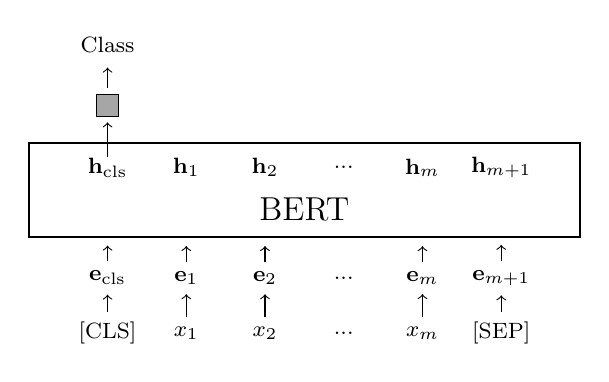
\begin{tikzpicture}
	
\def\vstep{1.3cm}
\def\ssep{1.0cm}

\tikzstyle{enode} = [minimum width=9*\nodestep,minimum height=1.4*\nodestep,inner sep=2pt,draw,thick];

\begin{scope}

%%%%%% train the encoder

\node [anchor=west] (w0) at (0,0) {\footnotesize{$[\mathrm{CLS}]$}};
\node [anchor=center] (w1) at ([xshift=\ssep]w0.center) {\footnotesize{$x_1$}};
\node [anchor=center] (w2) at ([xshift=\ssep]w1.center) {\footnotesize{$x_2$}};
\node [anchor=center] (w3) at ([xshift=\ssep]w2.center) {\footnotesize{$...$}};
\node [anchor=center] (w4) at ([xshift=\ssep]w3.center) {\footnotesize{$x_m$}};
\node [anchor=center] (w5) at ([xshift=\ssep]w4.center) {\footnotesize{$[\mathrm{SEP}]$}};

\node [anchor=center] (e0) at ([yshift=0.7*\ssep]w0.center) {\footnotesize{$\mathbf{e}_{\mathrm{cls}}$}};
\node [anchor=center] (e1) at ([yshift=0.7*\ssep]w1.center) {\footnotesize{$\mathbf{e}_1$}};
\node [anchor=center] (e2) at ([yshift=0.7*\ssep]w2.center) {\footnotesize{$\mathbf{e}_2$}};
\node [anchor=center] (e3) at ([yshift=0.7*\ssep]w3.center) {\footnotesize{$...$}};
\node [anchor=center] (e4) at ([yshift=0.7*\ssep]w4.center) {\footnotesize{$\mathbf{e}_{m}$}};
\node [anchor=center] (e5) at ([yshift=0.7*\ssep]w5.center) {\footnotesize{$\mathbf{e}_{m+1}$}};

\draw [->] (w0.north) -- (e0.south);
\draw [->] (w1.north) -- (e1.south);
\draw [->] (w2.north) -- (e2.south);
%\draw [->] (w3.north) -- (e3.south);
\draw [->] (w4.north) -- (e4.south);
\draw [->] (w5.north) -- (e5.south);

\draw [->] (e0.north) -- ([yshift=0.2*\ssep]e0.north);
\draw [->] (e1.north) -- ([yshift=0.2*\ssep]e1.north);
\draw [->] (e2.north) -- ([yshift=0.2*\ssep]e2.north);
%\draw [->] (e3.north) -- ([yshift=0.2*\ssep]e3.north);
\draw [->] (e4.north) -- ([yshift=0.2*\ssep]e4.north);
\draw [->] (e5.north) -- ([yshift=0.2*\ssep]e5.north);

\node [anchor=south,minimum width=7*\ssep,minimum height=1.2*\ssep,draw,thick] (encoder) at ([yshift=1.0*\ssep,xshift=0.5*\ssep]w2.north) {};

\node [anchor=center] (h0) at ([yshift=2.1*\ssep]w0.center) {\footnotesize{$\mathbf{h}_{\mathrm{cls}}$}};
\node [anchor=center] (h1) at ([yshift=2.1*\ssep]w1.center) {\footnotesize{$\mathbf{h}_1$}};
\node [anchor=center] (h2) at ([yshift=2.1*\ssep]w2.center) {\footnotesize{$\mathbf{h}_2$}};
\node [anchor=center] (h3) at ([yshift=2.1*\ssep]w3.center) {\footnotesize{$...$}};
\node [anchor=center] (h4) at ([yshift=2.1*\ssep]w4.center) {\footnotesize{$\mathbf{h}_m$}};
\node [anchor=center] (h5) at ([yshift=2.1*\ssep]w5.center) {\footnotesize{$\mathbf{h}_{m+1}$}};

\node [anchor=south,minimum height=0.8em,minimum width=0.8em,draw,fill=gray!70] (s0) at ([yshift=0.4*\ssep]h0.north) {};

\draw [->] ([yshift=-3pt]h0.north) -- ([yshift=-2pt]s0.south);

\node [anchor=south] (o0) at ([yshift=0.4*\ssep]s0.north) {\footnotesize{Class}};

\draw [->] ([yshift=2pt]s0.north) -- ([yshift=0.4*\ssep-2pt]s0.north);

\node [anchor=south] (encodercaption) at ([yshift=0.1cm]encoder.south) {\large{BERT}};

\end{scope}
	
\end{tikzpicture}

\caption{BERT-based classification for a single text.Here the gray box denotes the prediction network. }
\label{fig:bert-app-classification-single-text}
\end{figure}

    \noindent Many NLP problems can be categorized as text classification tasks, and there have been several text classification benchmarks for evaluating pre-trained models. For example, we can classify texts by their grammatical correctness (grammaticality) or emotional tone (sentiment)~\cite{socher-etal:2013recursive,warstadt-etal:2019neural}. Note that the prediction network could be any classification model, such as a deep neural network or a more traditional classification model. The entire model can then be trained or fine-tuned in the manner of a standard classification model. For example, the prediction network can be simply a Softmax layer and the model parameters can be optimized by maximizing the probabilities of the correct labels.

\item \vspace{0.3em} \textbf{Classification} (Pair of Texts). Classification can also be performed on a pair of texts. Suppose we have two texts, $x_1 \cdots x_m$ and $y_1 \cdots y_n$. We can concatenate these texts to form a single sequence with length $\mathrm{len}$. Then, we predict a label for this combined text sequence based on the $\mathbf{h}_{\mathrm{cls}}$ vector, as shown in Figure~\ref{fig:bert-app-classification-two-texts}.

\begin{figure}[!ht]
\centering
% !Mode:: "TeX:UTF-8"
% !TEX encoding = UTF-8 Unicode

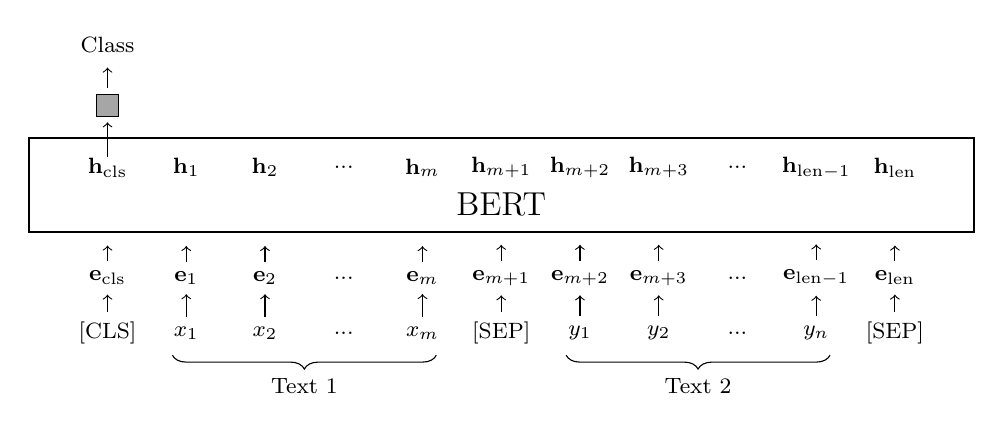
\begin{tikzpicture}
	
\def\vstep{1.3cm}
\def\ssep{1.0cm}

\tikzstyle{enode} = [minimum width=9*\nodestep,minimum height=1.4*\nodestep,inner sep=2pt,draw,thick];

\begin{scope}

%%%%%% train the encoder

\node [anchor=west] (w0) at (0,0) {\footnotesize{$[\mathrm{CLS}]$}};
\node [anchor=center] (w1) at ([xshift=\ssep]w0.center) {\footnotesize{$x_1$}};
\node [anchor=center] (w2) at ([xshift=\ssep]w1.center) {\footnotesize{$x_2$}};
\node [anchor=center] (w3) at ([xshift=\ssep]w2.center) {\footnotesize{$...$}};
\node [anchor=center] (w4) at ([xshift=\ssep]w3.center) {\footnotesize{$x_m$}};
\node [anchor=center] (w5) at ([xshift=\ssep]w4.center) {\footnotesize{$[\mathrm{SEP}]$}};
\node [anchor=center] (w6) at ([xshift=\ssep]w5.center) {\footnotesize{$y_1$}};
\node [anchor=center] (w7) at ([xshift=\ssep]w6.center) {\footnotesize{$y_2$}};
\node [anchor=center] (w8) at ([xshift=\ssep]w7.center) {\footnotesize{$...$}};
\node [anchor=center] (w9) at ([xshift=\ssep]w8.center) {\footnotesize{$y_n$}};
\node [anchor=center] (w10) at ([xshift=\ssep]w9.center) {\footnotesize{$[\mathrm{SEP}]$}};

\draw [decoration={brace,amplitude=5pt},decorate] ([xshift=0.5em,yshift=-0.8em]w4.center) -- ([xshift=-0.5em,yshift=-0.8em]w1.center) node [pos=0.5,below,yshift=-0.5em] (text1) {\footnotesize{Text 1}};

\draw [decoration={brace,amplitude=5pt},decorate] ([xshift=0.5em,yshift=-0.8em]w9.center) -- ([xshift=-0.5em,yshift=-0.8em]w6.center) node [pos=0.5,below,yshift=-0.5em] (text2) {\footnotesize{Text 2}};

\node [anchor=center] (e0) at ([yshift=0.7*\ssep]w0.center) {\footnotesize{$\mathbf{e}_{\mathrm{cls}}$}};
\node [anchor=center] (e1) at ([yshift=0.7*\ssep]w1.center) {\footnotesize{$\mathbf{e}_1$}};
\node [anchor=center] (e2) at ([yshift=0.7*\ssep]w2.center) {\footnotesize{$\mathbf{e}_2$}};
\node [anchor=center] (e3) at ([yshift=0.7*\ssep]w3.center) {\footnotesize{$...$}};
\node [anchor=center] (e4) at ([yshift=0.7*\ssep]w4.center) {\footnotesize{$\mathbf{e}_{m}$}};
\node [anchor=center] (e5) at ([yshift=0.7*\ssep]w5.center) {\footnotesize{$\mathbf{e}_{m+1}$}};
\node [anchor=center] (e6) at ([yshift=0.7*\ssep]w6.center) {\footnotesize{$\mathbf{e}_{m+2}$}};
\node [anchor=center] (e7) at ([yshift=0.7*\ssep]w7.center) {\footnotesize{$\mathbf{e}_{m+3}$}};
\node [anchor=center] (e8) at ([yshift=0.7*\ssep]w8.center) {\footnotesize{$...$}};
\node [anchor=center] (e9) at ([yshift=0.7*\ssep]w9.center) {\footnotesize{$\mathbf{e}_{\mathrm{len}-1}$}};
\node [anchor=center] (e10) at ([yshift=0.7*\ssep]w10.center) {\footnotesize{$\mathbf{e}_{\mathrm{len}}$}};

\draw [->] (w0.north) -- (e0.south);
\draw [->] (w1.north) -- (e1.south);
\draw [->] (w2.north) -- (e2.south);
%\draw [->] (w3.north) -- (e3.south);
\draw [->] (w4.north) -- (e4.south);
\draw [->] (w5.north) -- (e5.south);
\draw [->] (w6.north) -- (e6.south);
\draw [->] (w7.north) -- (e7.south);
%\draw [->] (w8.north) -- (e8.south);
\draw [->] (w9.north) -- (e9.south);
\draw [->] (w10.north) -- (e10.south);

\draw [->] (e0.north) -- ([yshift=0.2*\ssep]e0.north);
\draw [->] (e1.north) -- ([yshift=0.2*\ssep]e1.north);
\draw [->] (e2.north) -- ([yshift=0.2*\ssep]e2.north);
%\draw [->] (e3.north) -- ([yshift=0.2*\ssep]e3.north);
\draw [->] (e4.north) -- ([yshift=0.2*\ssep]e4.north);
\draw [->] (e5.north) -- ([yshift=0.2*\ssep]e5.north);
\draw [->] (e6.north) -- ([yshift=0.2*\ssep]e6.north);
\draw [->] (e7.north) -- ([yshift=0.2*\ssep]e7.north);
%\draw [->] (e8.north) -- ([yshift=0.2*\ssep]e8.north);
\draw [->] (e9.north) -- ([yshift=0.2*\ssep]e9.north);
\draw [->] (e10.north) -- ([yshift=0.2*\ssep]e10.north);

\node [anchor=south,minimum width=12*\ssep,minimum height=1.2*\ssep,draw,thick] (encoder) at ([yshift=1.0*\ssep,xshift=0.0*\ssep]w5.north) {};

\node [anchor=center] (h0) at ([yshift=2.1*\ssep]w0.center) {\footnotesize{$\mathbf{h}_{\mathrm{cls}}$}};
\node [anchor=center] (h1) at ([yshift=2.1*\ssep]w1.center) {\footnotesize{$\mathbf{h}_1$}};
\node [anchor=center] (h2) at ([yshift=2.1*\ssep]w2.center) {\footnotesize{$\mathbf{h}_2$}};
\node [anchor=center] (h3) at ([yshift=2.1*\ssep]w3.center) {\footnotesize{$...$}};
\node [anchor=center] (h4) at ([yshift=2.1*\ssep]w4.center) {\footnotesize{$\mathbf{h}_m$}};
\node [anchor=center] (h5) at ([yshift=2.1*\ssep]w5.center) {\footnotesize{$\mathbf{h}_{m+1}$}};
\node [anchor=center] (h6) at ([yshift=2.1*\ssep]w6.center) {\footnotesize{$\mathbf{h}_{m+2}$}};
\node [anchor=center] (h7) at ([yshift=2.1*\ssep]w7.center) {\footnotesize{$\mathbf{h}_{m+3}$}};
\node [anchor=center] (h8) at ([yshift=2.1*\ssep]w8.center) {\footnotesize{$...$}};
\node [anchor=center] (h9) at ([yshift=2.1*\ssep]w9.center) {\footnotesize{$\mathbf{h}_{\mathrm{len}-1}$}};
\node [anchor=center] (h10) at ([yshift=2.1*\ssep]w10.center) {\footnotesize{$\mathbf{h}_{\mathrm{len}}$}};

\node [anchor=south,minimum height=0.8em,minimum width=0.8em,draw,fill=gray!70] (s0) at ([yshift=0.4*\ssep]h0.north) {};

\draw [->] ([yshift=-3pt]h0.north) -- ([yshift=-2pt]s0.south);

\node [anchor=south] (o0) at ([yshift=0.4*\ssep]s0.north) {\footnotesize{Class}};

\draw [->] ([yshift=2pt]s0.north) -- ([yshift=0.4*\ssep-2pt]s0.north);

\node [anchor=south] (encodercaption) at ([yshift=0.1cm]encoder.south) {\large{BERT}};

\end{scope}
	
\end{tikzpicture}

\caption{BERT-based classification for a pair of texts.Here, $\mathrm{len} = n + m + 2$.}
\label{fig:bert-app-classification-two-texts}
\end{figure}

    \noindent Text pair classification covers several problems, including semantic equivalence judgement (determine whether two texts are semantically equivalent)~\cite{dolan-brockett:2005automatically}, text entailment judgement (determine whether a hypothesis can be logically inferred or entailed from a premise)~\cite{bentivogli-giampiccolo:2011rte,williams-etal:2018broad}, grounded commonsense inference (determine whether an event is likely to happen given its context)~\cite{zellers-etal:2018swag}, and question-answering inference (determine whether an answer corresponds to a given question).

\item \vspace{0.3em} \textbf{Regression}. Instead of generating a label distribution, we can have the prediction network output a real-valued score. For example, by adding a Sigmoid layer to the prediction network, the system can be employed to compute the similarity between two given sentences. The architecture is the same as that of BERT-based classification systems, with only the output layer changed, as shown in Figure~\ref{fig:bert-app-regression-two-texts}.

\begin{figure}[!ht]
\centering
% !Mode:: "TeX:UTF-8"
% !TEX encoding = UTF-8 Unicode

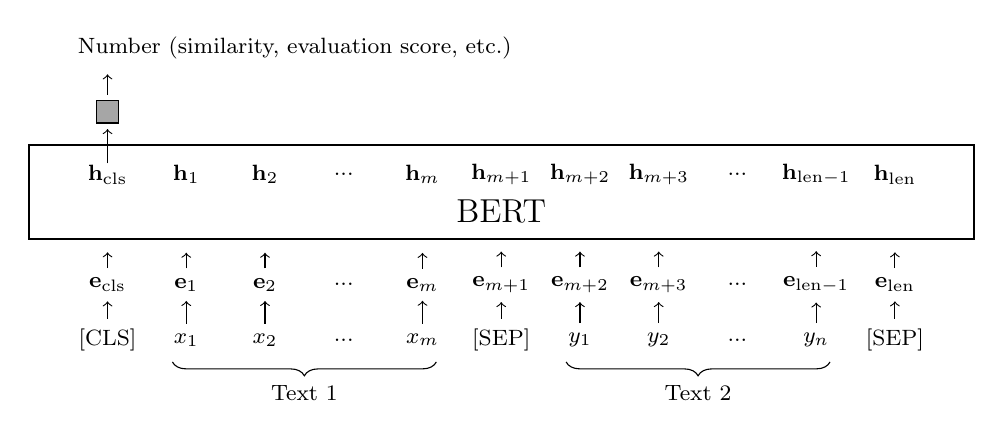
\begin{tikzpicture}
	
\def\vstep{1.3cm}
\def\ssep{1.0cm}

\tikzstyle{enode} = [minimum width=9*\nodestep,minimum height=1.4*\nodestep,inner sep=2pt,draw,thick];

\begin{scope}

%%%%%% train the encoder

\node [anchor=west] (w0) at (0,0) {\footnotesize{$[\mathrm{CLS}]$}};
\node [anchor=center] (w1) at ([xshift=\ssep]w0.center) {\footnotesize{$x_1$}};
\node [anchor=center] (w2) at ([xshift=\ssep]w1.center) {\footnotesize{$x_2$}};
\node [anchor=center] (w3) at ([xshift=\ssep]w2.center) {\footnotesize{$...$}};
\node [anchor=center] (w4) at ([xshift=\ssep]w3.center) {\footnotesize{$x_m$}};
\node [anchor=center] (w5) at ([xshift=\ssep]w4.center) {\footnotesize{$[\mathrm{SEP}]$}};
\node [anchor=center] (w6) at ([xshift=\ssep]w5.center) {\footnotesize{$y_1$}};
\node [anchor=center] (w7) at ([xshift=\ssep]w6.center) {\footnotesize{$y_2$}};
\node [anchor=center] (w8) at ([xshift=\ssep]w7.center) {\footnotesize{$...$}};
\node [anchor=center] (w9) at ([xshift=\ssep]w8.center) {\footnotesize{$y_n$}};
\node [anchor=center] (w10) at ([xshift=\ssep]w9.center) {\footnotesize{$[\mathrm{SEP}]$}};

\draw [decoration={brace,amplitude=5pt},decorate] ([xshift=0.5em,yshift=-0.8em]w4.center) -- ([xshift=-0.5em,yshift=-0.8em]w1.center) node [pos=0.5,below,yshift=-0.5em] (text1) {\footnotesize{Text 1}};

\draw [decoration={brace,amplitude=5pt},decorate] ([xshift=0.5em,yshift=-0.8em]w9.center) -- ([xshift=-0.5em,yshift=-0.8em]w6.center) node [pos=0.5,below,yshift=-0.5em] (text2) {\footnotesize{Text 2}};

\node [anchor=center] (e0) at ([yshift=0.7*\ssep]w0.center) {\footnotesize{$\mathbf{e}_{\mathrm{cls}}$}};
\node [anchor=center] (e1) at ([yshift=0.7*\ssep]w1.center) {\footnotesize{$\mathbf{e}_1$}};
\node [anchor=center] (e2) at ([yshift=0.7*\ssep]w2.center) {\footnotesize{$\mathbf{e}_2$}};
\node [anchor=center] (e3) at ([yshift=0.7*\ssep]w3.center) {\footnotesize{$...$}};
\node [anchor=center] (e4) at ([yshift=0.7*\ssep]w4.center) {\footnotesize{$\mathbf{e}_{m}$}};
\node [anchor=center] (e5) at ([yshift=0.7*\ssep]w5.center) {\footnotesize{$\mathbf{e}_{m+1}$}};
\node [anchor=center] (e6) at ([yshift=0.7*\ssep]w6.center) {\footnotesize{$\mathbf{e}_{m+2}$}};
\node [anchor=center] (e7) at ([yshift=0.7*\ssep]w7.center) {\footnotesize{$\mathbf{e}_{m+3}$}};
\node [anchor=center] (e8) at ([yshift=0.7*\ssep]w8.center) {\footnotesize{$...$}};
\node [anchor=center] (e9) at ([yshift=0.7*\ssep]w9.center) {\footnotesize{$\mathbf{e}_{\mathrm{len}-1}$}};
\node [anchor=center] (e10) at ([yshift=0.7*\ssep]w10.center) {\footnotesize{$\mathbf{e}_{\mathrm{len}}$}};

\draw [->] (w0.north) -- (e0.south);
\draw [->] (w1.north) -- (e1.south);
\draw [->] (w2.north) -- (e2.south);
%\draw [->] (w3.north) -- (e3.south);
\draw [->] (w4.north) -- (e4.south);
\draw [->] (w5.north) -- (e5.south);
\draw [->] (w6.north) -- (e6.south);
\draw [->] (w7.north) -- (e7.south);
%\draw [->] (w8.north) -- (e8.south);
\draw [->] (w9.north) -- (e9.south);
\draw [->] (w10.north) -- (e10.south);

\draw [->] (e0.north) -- ([yshift=0.2*\ssep]e0.north);
\draw [->] (e1.north) -- ([yshift=0.2*\ssep]e1.north);
\draw [->] (e2.north) -- ([yshift=0.2*\ssep]e2.north);
%\draw [->] (e3.north) -- ([yshift=0.2*\ssep]e3.north);
\draw [->] (e4.north) -- ([yshift=0.2*\ssep]e4.north);
\draw [->] (e5.north) -- ([yshift=0.2*\ssep]e5.north);
\draw [->] (e6.north) -- ([yshift=0.2*\ssep]e6.north);
\draw [->] (e7.north) -- ([yshift=0.2*\ssep]e7.north);
%\draw [->] (e8.north) -- ([yshift=0.2*\ssep]e8.north);
\draw [->] (e9.north) -- ([yshift=0.2*\ssep]e9.north);
\draw [->] (e10.north) -- ([yshift=0.2*\ssep]e10.north);

\node [anchor=south,minimum width=12*\ssep,minimum height=1.2*\ssep,draw,thick] (encoder) at ([yshift=1.0*\ssep,xshift=0.0*\ssep]w5.north) {};

\node [anchor=center] (h0) at ([yshift=2.1*\ssep]w0.center) {\footnotesize{$\mathbf{h}_{\mathrm{cls}}$}};
\node [anchor=center] (h1) at ([yshift=2.1*\ssep]w1.center) {\footnotesize{$\mathbf{h}_1$}};
\node [anchor=center] (h2) at ([yshift=2.1*\ssep]w2.center) {\footnotesize{$\mathbf{h}_2$}};
\node [anchor=center] (h3) at ([yshift=2.1*\ssep]w3.center) {\footnotesize{$...$}};
\node [anchor=center] (h4) at ([yshift=2.1*\ssep]w4.center) {\footnotesize{$\mathbf{h}_m$}};
\node [anchor=center] (h5) at ([yshift=2.1*\ssep]w5.center) {\footnotesize{$\mathbf{h}_{m+1}$}};
\node [anchor=center] (h6) at ([yshift=2.1*\ssep]w6.center) {\footnotesize{$\mathbf{h}_{m+2}$}};
\node [anchor=center] (h7) at ([yshift=2.1*\ssep]w7.center) {\footnotesize{$\mathbf{h}_{m+3}$}};
\node [anchor=center] (h8) at ([yshift=2.1*\ssep]w8.center) {\footnotesize{$...$}};
\node [anchor=center] (h9) at ([yshift=2.1*\ssep]w9.center) {\footnotesize{$\mathbf{h}_{\mathrm{len}-1}$}};
\node [anchor=center] (h10) at ([yshift=2.1*\ssep]w10.center) {\footnotesize{$\mathbf{h}_{\mathrm{len}}$}};

\node [anchor=south,minimum height=0.8em,minimum width=0.8em,draw,fill=gray!70] (s0) at ([yshift=0.4*\ssep]h0.north) {};

\draw [->] ([yshift=-3pt]h0.north) -- ([yshift=-2pt]s0.south);

\node [anchor=south west] (o0) at ([yshift=0.4*\ssep,xshift=-0.5cm]s0.north) {\footnotesize{Number} (similarity, evaluation score, etc.)};

\draw [->] ([yshift=2pt]s0.north) -- ([yshift=0.4*\ssep-2pt]s0.north);

\node [anchor=south] (encodercaption) at ([yshift=0.1cm]encoder.south) {\large{BERT}};

\end{scope}
	
\end{tikzpicture}

\caption{BERT-based regression for a pair of texts.}
\label{fig:bert-app-regression-two-texts}
\end{figure}

    For training or fine-tuning, we can minimize the regression loss of the model output as usual.

\item \vspace{0.3em} \textbf{Sequence Labeling}. Sequence labeling is a machine learning approach applicable to a wide range of NLP problems. This approach assigns a label to each token in an input sequence, and some linguistic annotations can then be derived from this sequence of labels. An example of sequence labeling in NLP is part-of-speech (POS) tagging. We label each word in a sentence with its corresponding POS tag. Another example is named entity recognition (NER) in which we label each word with an NER tag, and named entities are identified using these tags. See Figure~\ref{fig:bert-app-sequence-labeling} for an illustration of the model architecture for NER.

\begin{figure}[!ht]
\centering
% !Mode:: "TeX:UTF-8"
% !TEX encoding = UTF-8 Unicode

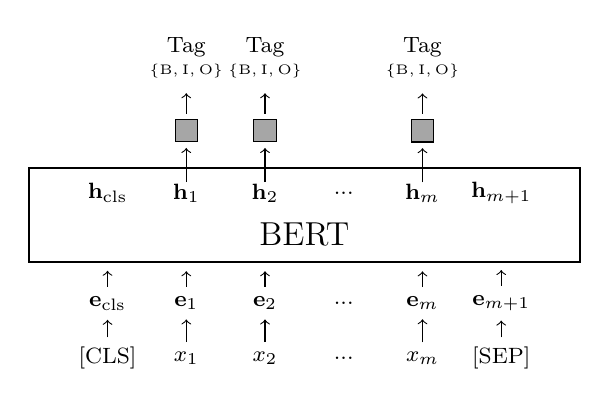
\begin{tikzpicture}
	
\def\vstep{1.3cm}
\def\ssep{1.0cm}

\tikzstyle{enode} = [minimum width=9*\nodestep,minimum height=1.4*\nodestep,inner sep=2pt,draw,thick];

\begin{scope}

%%%%%% train the encoder

\node [anchor=west] (w0) at (0,0) {\footnotesize{$[\mathrm{CLS}]$}};
\node [anchor=center] (w1) at ([xshift=\ssep]w0.center) {\footnotesize{$x_1$}};
\node [anchor=center] (w2) at ([xshift=\ssep]w1.center) {\footnotesize{$x_2$}};
\node [anchor=center] (w3) at ([xshift=\ssep]w2.center) {\footnotesize{$...$}};
\node [anchor=center] (w4) at ([xshift=\ssep]w3.center) {\footnotesize{$x_m$}};
\node [anchor=center] (w5) at ([xshift=\ssep]w4.center) {\footnotesize{$[\mathrm{SEP}]$}};

\node [anchor=center] (e0) at ([yshift=0.7*\ssep]w0.center) {\footnotesize{$\mathbf{e}_{\mathrm{cls}}$}};
\node [anchor=center] (e1) at ([yshift=0.7*\ssep]w1.center) {\footnotesize{$\mathbf{e}_1$}};
\node [anchor=center] (e2) at ([yshift=0.7*\ssep]w2.center) {\footnotesize{$\mathbf{e}_2$}};
\node [anchor=center] (e3) at ([yshift=0.7*\ssep]w3.center) {\footnotesize{$...$}};
\node [anchor=center] (e4) at ([yshift=0.7*\ssep]w4.center) {\footnotesize{$\mathbf{e}_{m}$}};
\node [anchor=center] (e5) at ([yshift=0.7*\ssep]w5.center) {\footnotesize{$\mathbf{e}_{m+1}$}};

\draw [->] (w0.north) -- (e0.south);
\draw [->] (w1.north) -- (e1.south);
\draw [->] (w2.north) -- (e2.south);
%\draw [->] (w3.north) -- (e3.south);
\draw [->] (w4.north) -- (e4.south);
\draw [->] (w5.north) -- (e5.south);

\draw [->] (e0.north) -- ([yshift=0.2*\ssep]e0.north);
\draw [->] (e1.north) -- ([yshift=0.2*\ssep]e1.north);
\draw [->] (e2.north) -- ([yshift=0.2*\ssep]e2.north);
%\draw [->] (e3.north) -- ([yshift=0.2*\ssep]e3.north);
\draw [->] (e4.north) -- ([yshift=0.2*\ssep]e4.north);
\draw [->] (e5.north) -- ([yshift=0.2*\ssep]e5.north);

\node [anchor=south,minimum width=7*\ssep,minimum height=1.2*\ssep,draw,thick] (encoder) at ([yshift=1.0*\ssep,xshift=0.5*\ssep]w2.north) {};

\node [anchor=center] (h0) at ([yshift=2.1*\ssep]w0.center) {\footnotesize{$\mathbf{h}_{\mathrm{cls}}$}};
\node [anchor=center] (h1) at ([yshift=2.1*\ssep]w1.center) {\footnotesize{$\mathbf{h}_1$}};
\node [anchor=center] (h2) at ([yshift=2.1*\ssep]w2.center) {\footnotesize{$\mathbf{h}_2$}};
\node [anchor=center] (h3) at ([yshift=2.1*\ssep]w3.center) {\footnotesize{$...$}};
\node [anchor=center] (h4) at ([yshift=2.1*\ssep]w4.center) {\footnotesize{$\mathbf{h}_m$}};
\node [anchor=center] (h5) at ([yshift=2.1*\ssep]w5.center) {\footnotesize{$\mathbf{h}_{m+1}$}};

\node [anchor=south,minimum height=0.8em,minimum width=0.8em,draw,fill=gray!70] (s1) at ([yshift=0.4*\ssep]h1.north) {};
\node [anchor=south,minimum height=0.8em,minimum width=0.8em,draw,fill=gray!70] (s2) at ([yshift=0.4*\ssep]h2.north) {};
\node [anchor=south,minimum height=0.8em,minimum width=0.8em,draw,fill=gray!70] (s4) at ([yshift=0.4*\ssep]h4.north) {};

\draw [->] ([yshift=-3pt]h1.north) -- ([yshift=-2pt]s1.south);
\draw [->] ([yshift=-3pt]h2.north) -- ([yshift=-2pt]s2.south);
\draw [->] ([yshift=-3pt]h4.north) -- ([yshift=-2pt]s4.south);

\node [anchor=south] (o1) at ([yshift=0.4*\ssep]s1.north) {\tiny{$\{\mathrm{B},\mathrm{I},\mathrm{O}\}$}};
\node [anchor=south] (o2) at ([yshift=0.4*\ssep]s2.north) {\tiny{$\{\mathrm{B},\mathrm{I},\mathrm{O}\}$}};
\node [anchor=south] (o4) at ([yshift=0.4*\ssep]s4.north) {\tiny{$\{\mathrm{B},\mathrm{I},\mathrm{O}\}$}};
\node [anchor=south] (oo1) at ([yshift=-0.15cm]o1.north) {\footnotesize{Tag}};
\node [anchor=south] (oo2) at ([yshift=-0.15cm]o2.north) {\footnotesize{Tag}};
\node [anchor=south] (oo4) at ([yshift=-0.15cm]o4.north) {\footnotesize{Tag}};

\draw [->] ([yshift=2pt]s1.north) -- ([yshift=0.4*\ssep-2pt]s1.north);
\draw [->] ([yshift=2pt]s2.north) -- ([yshift=0.4*\ssep-2pt]s2.north);
\draw [->] ([yshift=2pt]s4.north) -- ([yshift=0.4*\ssep-2pt]s4.north);

\node [anchor=south] (encodercaption) at ([yshift=0.1cm]encoder.south) {\large{BERT}};

\end{scope}
	
\end{tikzpicture}

\caption{BERT-based sequence labeling for named entity recognition.Here $\{\mathrm{B}, \mathrm{I}, \mathrm{O}\}$ is the tag set of NER.}
\label{fig:bert-app-sequence-labeling}
\end{figure}

    \noindent  In this model, we use the BIO tagging scheme to represent named entities. For example, $\mathrm{B}\textrm{-}\mathrm{ORG}$ means the beginning of an organization, $\mathrm{I}\textrm{-}\mathrm{ORG}$ means the word is inside an organization, and $\mathrm{O}$ means the word does not belong to any named entity. This NER model can output a distribution over the tag set at each position, denoted as $\mathbf{p}_i$. The training or fine-tuning of the model can be performed over these distributions $\{\mathbf{p}_1,\cdots,\mathbf{p}_m\}$. For example, suppose $p_i(\mathrm{tag}_i)$ is the probability of the correct tag at position $i$. The training loss can be defined to be the negative log-likelihood
    \begin{eqnarray}
    \mathrm{Loss} & = & -\frac{1}{m} \sum_{i=1}^{m} \log p_i(\mathrm{tag}_i).
    \end{eqnarray}

    Finding the best label sequence given a trained NER model is a well-studied problem in NLP. This is often achieved via dynamic programming, which, in the context of path finding over a lattice, has linear complexity~\cite{huang-etal:2009dynamic}.

\item \vspace{0.3em} \textbf{Span Prediction}. Some NLP tasks require predicting a span in a text. A common example is reading comprehension. In this task, we are given a query $x_1 \cdots x_m$ and a context text $y_1 \cdots y_n$. The goal is to identify a continuous span in $y_1 \cdots y_n$ that best answers the query. This problem can be framed as a sequence labeling-like task in which we predict a label for each $y_j$ to indicate the beginning or ending of the span. Following \citet{seo-etal:2017bidirectional}, we add two networks on top of the BERT output for $y_j$: one for generating the probability of $y_j$ being the beginning of the span (denoted by $p_j^{\mathrm{beg}}$), and one for generating the probability of $y_j$ being the ending of the span (denoted by $p_j^{\mathrm{end}}$). The resulting model architecture is shown in Figure~\ref{fig:bert-app-span-prediction}.

\begin{figure}[!ht]
\centering
% !Mode:: "TeX:UTF-8"
% !TEX encoding = UTF-8 Unicode

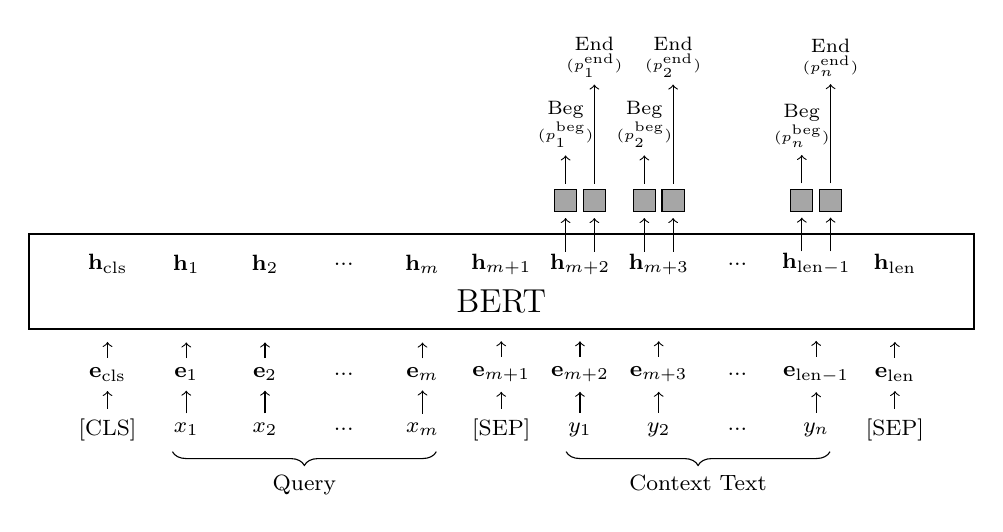
\begin{tikzpicture}
	
\def\vstep{1.3cm}
\def\ssep{1.0cm}

\tikzstyle{enode} = [minimum width=9*\nodestep,minimum height=1.4*\nodestep,inner sep=2pt,draw,thick];

\begin{scope}

%%%%%% train the encoder

\node [anchor=west] (w0) at (0,0) {\footnotesize{$[\mathrm{CLS}]$}};
\node [anchor=center] (w1) at ([xshift=\ssep]w0.center) {\footnotesize{$x_1$}};
\node [anchor=center] (w2) at ([xshift=\ssep]w1.center) {\footnotesize{$x_2$}};
\node [anchor=center] (w3) at ([xshift=\ssep]w2.center) {\footnotesize{$...$}};
\node [anchor=center] (w4) at ([xshift=\ssep]w3.center) {\footnotesize{$x_m$}};
\node [anchor=center] (w5) at ([xshift=\ssep]w4.center) {\footnotesize{$[\mathrm{SEP}]$}};
\node [anchor=center] (w6) at ([xshift=\ssep]w5.center) {\footnotesize{$y_1$}};
\node [anchor=center] (w7) at ([xshift=\ssep]w6.center) {\footnotesize{$y_2$}};
\node [anchor=center] (w8) at ([xshift=\ssep]w7.center) {\footnotesize{$...$}};
\node [anchor=center] (w9) at ([xshift=\ssep]w8.center) {\footnotesize{$y_n$}};
\node [anchor=center] (w10) at ([xshift=\ssep]w9.center) {\footnotesize{$[\mathrm{SEP}]$}};

\draw [decoration={brace,amplitude=5pt},decorate] ([xshift=0.5em,yshift=-0.8em]w4.center) -- ([xshift=-0.5em,yshift=-0.8em]w1.center) node [pos=0.5,below,yshift=-0.5em] (text1) {\footnotesize{Query}};

\draw [decoration={brace,amplitude=5pt},decorate] ([xshift=0.5em,yshift=-0.8em]w9.center) -- ([xshift=-0.5em,yshift=-0.8em]w6.center) node [pos=0.5,below,yshift=-0.5em] (text2) {\footnotesize{Context Text}};

\node [anchor=center] (e0) at ([yshift=0.7*\ssep]w0.center) {\footnotesize{$\mathbf{e}_{\mathrm{cls}}$}};
\node [anchor=center] (e1) at ([yshift=0.7*\ssep]w1.center) {\footnotesize{$\mathbf{e}_1$}};
\node [anchor=center] (e2) at ([yshift=0.7*\ssep]w2.center) {\footnotesize{$\mathbf{e}_2$}};
\node [anchor=center] (e3) at ([yshift=0.7*\ssep]w3.center) {\footnotesize{$...$}};
\node [anchor=center] (e4) at ([yshift=0.7*\ssep]w4.center) {\footnotesize{$\mathbf{e}_{m}$}};
\node [anchor=center] (e5) at ([yshift=0.7*\ssep]w5.center) {\footnotesize{$\mathbf{e}_{m+1}$}};
\node [anchor=center] (e6) at ([yshift=0.7*\ssep]w6.center) {\footnotesize{$\mathbf{e}_{m+2}$}};
\node [anchor=center] (e7) at ([yshift=0.7*\ssep]w7.center) {\footnotesize{$\mathbf{e}_{m+3}$}};
\node [anchor=center] (e8) at ([yshift=0.7*\ssep]w8.center) {\footnotesize{$...$}};
\node [anchor=center] (e9) at ([yshift=0.7*\ssep]w9.center) {\footnotesize{$\mathbf{e}_{\mathrm{len}-1}$}};
\node [anchor=center] (e10) at ([yshift=0.7*\ssep]w10.center) {\footnotesize{$\mathbf{e}_{\mathrm{len}}$}};

\draw [->] (w0.north) -- (e0.south);
\draw [->] (w1.north) -- (e1.south);
\draw [->] (w2.north) -- (e2.south);
%\draw [->] (w3.north) -- (e3.south);
\draw [->] (w4.north) -- (e4.south);
\draw [->] (w5.north) -- (e5.south);
\draw [->] (w6.north) -- (e6.south);
\draw [->] (w7.north) -- (e7.south);
%\draw [->] (w8.north) -- (e8.south);
\draw [->] (w9.north) -- (e9.south);
\draw [->] (w10.north) -- (e10.south);

\draw [->] (e0.north) -- ([yshift=0.2*\ssep]e0.north);
\draw [->] (e1.north) -- ([yshift=0.2*\ssep]e1.north);
\draw [->] (e2.north) -- ([yshift=0.2*\ssep]e2.north);
%\draw [->] (e3.north) -- ([yshift=0.2*\ssep]e3.north);
\draw [->] (e4.north) -- ([yshift=0.2*\ssep]e4.north);
\draw [->] (e5.north) -- ([yshift=0.2*\ssep]e5.north);
\draw [->] (e6.north) -- ([yshift=0.2*\ssep]e6.north);
\draw [->] (e7.north) -- ([yshift=0.2*\ssep]e7.north);
%\draw [->] (e8.north) -- ([yshift=0.2*\ssep]e8.north);
\draw [->] (e9.north) -- ([yshift=0.2*\ssep]e9.north);
\draw [->] (e10.north) -- ([yshift=0.2*\ssep]e10.north);

\node [anchor=south,minimum width=12*\ssep,minimum height=1.2*\ssep,draw,thick] (encoder) at ([yshift=1.0*\ssep,xshift=0.0*\ssep]w5.north) {};

\node [anchor=center] (h0) at ([yshift=2.1*\ssep]w0.center) {\footnotesize{$\mathbf{h}_{\mathrm{cls}}$}};
\node [anchor=center] (h1) at ([yshift=2.1*\ssep]w1.center) {\footnotesize{$\mathbf{h}_1$}};
\node [anchor=center] (h2) at ([yshift=2.1*\ssep]w2.center) {\footnotesize{$\mathbf{h}_2$}};
\node [anchor=center] (h3) at ([yshift=2.1*\ssep]w3.center) {\footnotesize{$...$}};
\node [anchor=center] (h4) at ([yshift=2.1*\ssep]w4.center) {\footnotesize{$\mathbf{h}_m$}};
\node [anchor=center] (h5) at ([yshift=2.1*\ssep]w5.center) {\footnotesize{$\mathbf{h}_{m+1}$}};
\node [anchor=center] (h6) at ([yshift=2.1*\ssep]w6.center) {\footnotesize{$\mathbf{h}_{m+2}$}};
\node [anchor=center] (h7) at ([yshift=2.1*\ssep]w7.center) {\footnotesize{$\mathbf{h}_{m+3}$}};
\node [anchor=center] (h8) at ([yshift=2.1*\ssep]w8.center) {\footnotesize{$...$}};
\node [anchor=center] (h9) at ([yshift=2.1*\ssep]w9.center) {\footnotesize{$\mathbf{h}_{\mathrm{len}-1}$}};
\node [anchor=center] (h10) at ([yshift=2.1*\ssep]w10.center) {\footnotesize{$\mathbf{h}_{\mathrm{len}}$}};

\node [anchor=south east,minimum height=0.8em,minimum width=0.8em,draw,fill=gray!70] (s6beg) at ([yshift=0.4*\ssep,xshift=-0.1em]h6.north) {};
\node [anchor=south west,minimum height=0.8em,minimum width=0.8em,draw,fill=gray!70] (s6end) at ([yshift=0.4*\ssep,xshift=0.1em]h6.north) {};

\node [anchor=south east,minimum height=0.8em,minimum width=0.8em,draw,fill=gray!70] (s7beg) at ([yshift=0.4*\ssep,xshift=-0.1em]h7.north) {};
\node [anchor=south west,minimum height=0.8em,minimum width=0.8em,draw,fill=gray!70] (s7end) at ([yshift=0.4*\ssep,xshift=0.1em]h7.north) {};

\node [anchor=south east,minimum height=0.8em,minimum width=0.8em,draw,fill=gray!70] (s9beg) at ([yshift=0.4*\ssep,xshift=-0.1em]h9.north) {};
\node [anchor=south west,minimum height=0.8em,minimum width=0.8em,draw,fill=gray!70] (s9end) at ([yshift=0.4*\ssep,xshift=0.1em]h9.north) {};

\draw [->] ([yshift=-0.5*\ssep]s6beg.south) -- ([yshift=-2pt]s6beg.south);
\draw [->] ([yshift=-0.5*\ssep]s6end.south) -- ([yshift=-2pt]s6end.south);

\draw [->] ([yshift=-0.5*\ssep]s7beg.south) -- ([yshift=-2pt]s7beg.south);
\draw [->] ([yshift=-0.5*\ssep]s7end.south) -- ([yshift=-2pt]s7end.south);

\draw [->] ([yshift=-0.5*\ssep]s9beg.south) -- ([yshift=-2pt]s9beg.south);
\draw [->] ([yshift=-0.5*\ssep]s9end.south) -- ([yshift=-2pt]s9end.south);s

\node [anchor=south] (o6beg) at ([yshift=0.4*\ssep]s6beg.north) {\tiny{$(p_1^{\mathrm{beg}})$}};
\node [anchor=south] (o6beg2) at ([yshift=-0.2cm]o6beg.north) {\scriptsize{$\mathrm{Beg}$}};
\node [anchor=south] (o6end) at ([yshift=1.3*\ssep]s6end.north) {\tiny{$(p_1^{\mathrm{end}})$}};
\node [anchor=south] (o6end2) at ([yshift=-0.2cm]o6end.north) {\scriptsize{$\mathrm{End}$}};

\node [anchor=south] (o7beg) at ([yshift=0.4*\ssep]s7beg.north) {\tiny{$(p_2^{\mathrm{beg}})$}};
\node [anchor=south] (o7beg2) at ([yshift=-0.2cm]o7beg.north) {\scriptsize{$\mathrm{Beg}$}};
\node [anchor=south] (o7end) at ([yshift=1.3*\ssep]s7end.north) {\tiny{$(p_2^{\mathrm{end}})$}};
\node [anchor=south] (o7end2) at ([yshift=-0.2cm]o7end.north) {\scriptsize{$\mathrm{End}$}};

\node [anchor=south] (o9beg) at ([yshift=0.4*\ssep]s9beg.north) {\tiny{$(p_n^{\mathrm{beg}})$}};
\node [anchor=south] (o9beg2) at ([yshift=-0.2cm]o9beg.north) {\scriptsize{$\mathrm{Beg}$}};
\node [anchor=south] (o9end) at ([yshift=1.3*\ssep]s9end.north) {\tiny{$(p_n^{\mathrm{end}})$}};
\node [anchor=south] (o9end2) at ([yshift=-0.2cm]o9end.north) {\scriptsize{$\mathrm{End}$}};

\draw [->] ([yshift=2pt]s6beg.north) -- ([yshift=0.5*\ssep-2pt]s6beg.north);
\draw [->] ([yshift=2pt]s6end.north) -- ([yshift=1.4*\ssep-2pt]s6end.north);

\draw [->] ([yshift=2pt]s7beg.north) -- ([yshift=0.5*\ssep-2pt]s7beg.north);
\draw [->] ([yshift=2pt]s7end.north) -- ([yshift=1.4*\ssep-2pt]s7end.north);

\draw [->] ([yshift=2pt]s9beg.north) -- ([yshift=0.5*\ssep-2pt]s9beg.north);
\draw [->] ([yshift=2pt]s9end.north) -- ([yshift=1.4*\ssep-2pt]s9end.north);

\node [anchor=south] (encodercaption) at ([yshift=0.1cm]encoder.south) {\large{BERT}};

\end{scope}
	
\end{tikzpicture}

\caption{BERT-based span prediction for reading comprehension.}
\label{fig:bert-app-span-prediction}
\end{figure}

    We pack the query and context text together to obtain the input sequence. The prediction networks are only applied to outputs for the context text, generating the probabilities $p_j^{\mathrm{beg}}$ and $p_j^{\mathrm{end}}$ at each position. The loss can be computed by summing the negative log likelihoods of the two models across the entire context text.
    \begin{eqnarray}
    \mathrm{Loss} & = & - \frac{1}{n} \sum_{j=1}^{n} \big( \log p_j^{\mathrm{beg}} + \log p_j^{\mathrm{end}} \big).
    \end{eqnarray}

    At test time, we search for the best span by
    \begin{eqnarray}
    (\hat{j}_1,\hat{j}_2) & = & \argmax_{1 \le j_1 \le j_2 \le n}\ \big( \log p_{j_1}^{\mathrm{beg}} + \log p_{j_2}^{\mathrm{end}} \big).
    \end{eqnarray}

\item \vspace{0.3em} \textbf{Encoding for Encoder-Decoder Models}. While our focus in this section has been primarily on language understanding problems, it is worth noting that BERT models can be applied to a broader range of NLP tasks. In fact, BERT models can be used in all the scenarios where we need to encode a piece of text. One application that we have not mentioned is text generation which includes a range of tasks such as machine translation, summarization, question answering, and dialogue generation. These tasks can be formulated as sequence-to-sequence problems: we use an encoder to represent the source text, and a decoder to generate the corresponding target text. A straightforward method to apply BERT models is to consider them as encoders. Before fine-tuning, we can initialize the parameters of the encoder with those from a pre-trained BERT model. Then, the encoder-decoder model can be fine-tuned on pairs of texts as usual. Figure~\ref{fig:bert-app-encoder-decoder} shows the architecture of a neural machine translation system where a BERT model is applied on the source side.

\begin{figure}[!ht]
\centering
% !Mode:: "TeX:UTF-8"
% !TEX encoding = UTF-8 Unicode

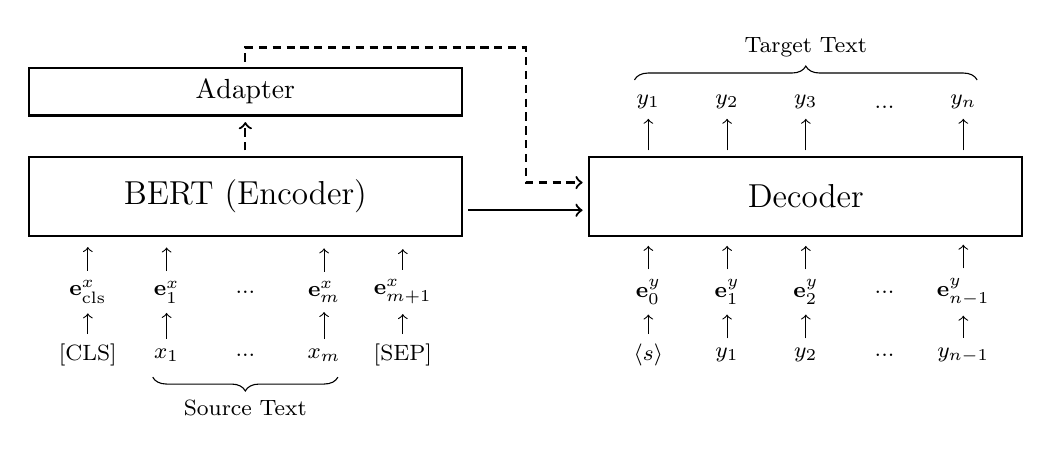
\begin{tikzpicture}
	
\def\vstep{1.3cm}
\def\ssep{1.0cm}

\tikzstyle{enode} = [minimum width=9*\nodestep,minimum height=1.4*\nodestep,inner sep=2pt,draw,thick];

%%%%%% encoder
\begin{scope}

\node [anchor=west] (w0) at (0,0) {\footnotesize{$[\mathrm{CLS}]$}};
\node [anchor=center] (w1) at ([xshift=\ssep]w0.center) {\footnotesize{$x_1$}};
\node [anchor=center] (w2) at ([xshift=\ssep]w1.center) {\footnotesize{$...$}};
\node [anchor=center] (w3) at ([xshift=\ssep]w2.center) {\footnotesize{$x_m$}};
\node [anchor=center] (w4) at ([xshift=\ssep]w3.center) {\footnotesize{$[\mathrm{SEP}]$}};


\draw [decoration={brace,amplitude=5pt},decorate] ([xshift=0.5em,yshift=-0.8em]w3.center) -- ([xshift=-0.5em,yshift=-0.8em]w1.center) node [pos=0.5,below,yshift=-0.5em] (text1) {\footnotesize{Source Text}};

\node [anchor=center] (e0) at ([yshift=0.8*\ssep]w0.center) {\footnotesize{$\mathbf{e}^{x}_{\mathrm{cls}}$}};
\node [anchor=center] (e1) at ([yshift=0.8*\ssep]w1.center) {\footnotesize{$\mathbf{e}^{x}_1$}};
\node [anchor=center] (e2) at ([yshift=0.8*\ssep]w2.center) {\footnotesize{$...$}};
\node [anchor=center] (e3) at ([yshift=0.8*\ssep]w3.center) {\footnotesize{$\mathbf{e}^{x}_{m}$}};
\node [anchor=center] (e4) at ([yshift=0.8*\ssep]w4.center) {\footnotesize{$\mathbf{e}^{x}_{m+1}$}};

\draw [->] (w0.north) -- (e0.south);
\draw [->] (w1.north) -- (e1.south);
%\draw [->] (w2.north) -- (e2.south);
\draw [->] (w3.north) -- (e3.south);
\draw [->] (w4.north) -- (e4.south);


\draw [->] (e0.north) -- ([yshift=0.3*\ssep]e0.north);
\draw [->] (e1.north) -- ([yshift=0.3*\ssep]e1.north);
%\draw [->] (e2.north) -- ([yshift=0.3*\ssep]e2.north);
\draw [->] (e3.north) -- ([yshift=0.3*\ssep]e3.north);
\draw [->] ([yshift=0]e4.north) -- ([yshift=0.3*\ssep-1pt]e4.north);

\node [anchor=south,minimum width=5.5*\ssep,minimum height=1.0*\ssep,draw,thick] (encoder) at ([yshift=1.2*\ssep + 0.3cm,xshift=0.0*\ssep]w2.center) {\large{BERT (Encoder)}};

\node [anchor=south,minimum width=5.5*\ssep,minimum height=0.6*\ssep,draw,thick] (adapter) at ([yshift=0.5*\ssep]encoder.north) {Adapter};

\end{scope}

%%%%%% decoder
\begin{scope}[xshift=7.3cm]

\node [anchor=west] (y0) at (0,0) {\footnotesize{$\langle s \rangle$}};
\node [anchor=center] (y1) at ([xshift=\ssep]y0.center) {\footnotesize{$y_1$}};
\node [anchor=center] (y2) at ([xshift=\ssep]y1.center) {\footnotesize{$y_2$}};
\node [anchor=center] (y3) at ([xshift=\ssep]y2.center) {\footnotesize{$...$}};
\node [anchor=center] (y4) at ([xshift=\ssep]y3.center) {\footnotesize{$y_{n-1}$}};

\node [anchor=center] (ey0) at ([yshift=0.8*\ssep]y0.center) {\footnotesize{$\mathbf{e}^{y}_{0}$}};
\node [anchor=center] (ey1) at ([yshift=0.8*\ssep]y1.center) {\footnotesize{$\mathbf{e}^{y}_{1}$}};
\node [anchor=center] (ey2) at ([yshift=0.8*\ssep]y2.center) {\footnotesize{$\mathbf{e}^{y}_{2}$}};
\node [anchor=center] (ey3) at ([yshift=0.8*\ssep]y3.center) {\footnotesize{$...$}};
\node [anchor=center] (ey4) at ([yshift=0.8*\ssep]y4.center) {\footnotesize{$\mathbf{e}^{y}_{n-1}$}};

\draw [->] (y0.north) -- (ey0.south);
\draw [->] (y1.north) -- (ey1.south);
\draw [->] (y2.north) -- (ey2.south);
%\draw [->] (y3.north) -- (ey3.south);
\draw [->] (y4.north) -- (ey4.south);

\draw [->] (ey0.north) -- ([yshift=0.3*\ssep]ey0.north);
\draw [->] (ey1.north) -- ([yshift=0.3*\ssep]ey1.north);
\draw [->] (ey2.north) -- ([yshift=0.3*\ssep]ey2.north);
%\draw [->] (ey3.north) -- ([yshift=0.3*\ssep]ey3.north);
\draw [->] (ey4.north) -- ([yshift=0.3*\ssep]ey4.north);

\node [anchor=south,minimum width=5.5*\ssep,minimum height=1.0*\ssep,draw,thick] (decoder) at ([yshift=1.2*\ssep + 0.3cm,xshift=0.0*\ssep]y2.center) {\large{Decoder}};

\node [anchor=south,minimum height=0.8em,minimum width=0.8em] (t0) at ([yshift=2.2*\ssep]ey0.center) {\footnotesize{$y_1$}};
\node [anchor=south,minimum height=0.8em,minimum width=0.8em] (t1) at ([yshift=2.2*\ssep]ey1.center) {\footnotesize{$y_2$}};
\node [anchor=south,minimum height=0.8em,minimum width=0.8em] (t2) at ([yshift=2.2*\ssep]ey2.center) {\footnotesize{$y_3$}};
\node [anchor=south,minimum height=0.8em,minimum width=0.8em] (t3) at ([yshift=2.2*\ssep]ey3.center) {\footnotesize{$...$}};
\node [anchor=south,minimum height=0.8em,minimum width=0.8em] (t4) at ([yshift=2.2*\ssep]ey4.center) {\footnotesize{$y_{n}$}};

\draw [->] ([yshift=-0.4*\ssep]t0.south) -- ([yshift=-0pt]t0.south);
\draw [->] ([yshift=-0.4*\ssep]t1.south) -- ([yshift=-0pt]t1.south);
\draw [->] ([yshift=-0.4*\ssep]t2.south) -- ([yshift=-0pt]t2.south);
%\draw [->] ([yshift=-0.4*\ssep]t3.south) -- ([yshift=-0pt]t3.south);
\draw [->] ([yshift=-0.4*\ssep]t4.south) -- ([yshift=-0pt]t4.south);

\draw [decoration={brace,amplitude=5pt},decorate] ([xshift=-0.5em,yshift=0.8em]t0.center) -- ([xshift=0.5em,yshift=0.8em]t4.center) node [pos=0.5,above,yshift=0.5em] (text2) {\footnotesize{Target Text}};

\draw [->,thick,densely dashed] ([yshift=2pt]encoder.north) -- ([yshift=-2pt]adapter.south);
\draw [->,thick,densely dashed] ([yshift=2pt]adapter.north) -- ([yshift=0.25*\ssep]adapter.north) -- ([yshift=0.25*\ssep,xshift=0.8*\ssep]adapter.north east) -- ([xshift=0.8*\ssep,yshift=0.5em]encoder.east) -- ([xshift=-2pt,yshift=0.5em]decoder.west);
\draw [->,thick] ([xshift=2pt,yshift=-0.5em]encoder.east) -- ([xshift=-2pt,yshift=-0.5em]decoder.west);

\end{scope}
	
\end{tikzpicture}

\caption{Using BERT as the encoder in an encoder-decoder model.Here $x_1 \cdots x_m$ denotes the source sequence, $y_1 \cdots y_n$ denotes the target sequence, $\mathbf{e}_{1}^{x} \cdots \mathbf{e}_{m}^{x}$ denotes the embedding sequence of $x_1 \cdots x_m$, and $\mathbf{e}_{1}^{y} \cdots \mathbf{e}_{n}^{y}$ denotes the embedding sequence of $y_1 \cdots y_n$. The adapter, which is optional, maps the output of the BERT model to the form that is better suited to the decoder.}
\label{fig:bert-app-encoder-decoder}
\end{figure}

\end{itemize}
\vspace{0.5em}

Fine-tuning BERT models is a complicated engineering problem, influenced by many factors, such as the amount of fine-tuning data, the model size, and the optimizer used in fine-tuning. In general, we wish to fine-tune these models sufficiently so that they can perform well in the downstream tasks. However, fine-tuning BERT models for specific tasks may lead to overfitting, which in turn reduces their ability to generalize to other tasks. For example, suppose we have a BERT model that performs well on a particular task. If we then fine-tune it for new tasks, this may decrease its performance on the original task. This problem is related to the \mindex{catastrophic forgetting} problem in continual training, where a neural network forgets previously learned information when updated on new samples. In practical applications, a common way to alleviate catastrophic forgetting is to add some old data into fine-tuning and train the model with more diverse data. Also, one may use methods specialized to catastrophic forgetting, such as experience replay~\cite{rolnick-etal:2019experience} and elastic weight consolidation~\cite{kirkpatrick-etal:2017overcoming}. The interested reader can refer to some surveys for more detailed discussions of this issue in continual learning~\cite{parisi-etal:2019continual,wang-etal:2023comprehensive,wang-etal:2023comprehensive2}.

%----------------------------------------------------------------------------------------
% NEW SECTION
%----------------------------------------------------------------------------------------

\section{Summary}

\noindent In this chapter we have introduced the general concept of pre-training in NLP. In particular, we have discussed self-supervised pre-training and its application to encoder-only, decoder-only, and encoder-decoder architectures. Moreover, we have presented and compared a variety of pre-training tasks for these architectures. As an example, we used BERT to illustrate how sequence models are pre-trained via masked language modeling and applied to different downstream tasks.

Recent years have shown remarkable progress in NLP, led by the large-scale use of self-supervised pre-training. Significant advances have been made across many tasks, not only in NLP but also in computer vision and other areas of AI. One idea behind these advances is that a significant amount of knowledge about the world can be learned by simply training these AI systems on huge amounts of unlabeled data. For example, a language model can learn some general knowledge of a language by repeatedly predicting masked words in large-scale text. As a result, this pre-trained language model can serve as a foundation model, which can be easily adapted to address specific downstream NLP tasks. This paradigm shift in NLP has enabled the development of powerful systems for language understanding, generation, and reasoning~\cite{manning:2022human}. However, it is important to recognize that we are still in the early stages of creating truly intelligent systems, and there is a long way to go. Nevertheless, large-scale pre-training has opened a door to intelligent systems that researchers have long aspired to develop, though several key research areas remain open for exploration, such as learning efficiently from limited data and acquiring complex reasoning and planning abilities.

Note that this chapter is mostly introductory and cannot cover all aspects of pre-training. For example, there are many methods to fine-tune a pre-trained model, offering different ways to adapt the model to diverse scenarios.  Moreover, large language models, which are considered one of the most significant achievements in AI in recent years, are not covered in this chapter. We leave the discussion of these topics to the following chapters.
